\documentclass[10pt,a4paper]{amsart}
\usepackage{amsmath,amssymb,amsthm,graphicx}
\usepackage{amsmath,amssymb,graphicx,xcolor,mathtools,listings}
\usepackage[no-math]{fontspec}
\newfontfamily\proofcodefont{DejaVu Sans}
\newfontfamily\proofwavefont{DejaVu Serif}
\lstset{basicstyle=\proofcodefont\tiny,breaklines=true,columns=fullflexible,keepspaces=true,escapeinside={(*@}{@*)}}
\title{Conditional equivalence of typed and untyped algorithmic conversion in dependent type theory}
\author{Meven Lennon-Bertrand}
\date{doi:10.4230/LIPIcs.FSCD.2025.27; CC BY4.0 (paper); MIT (author formal library)}
\begin{document}
\maketitle
\noindent\textit{Editorial note.} Paper https://drops.dagstuhl.de/entities/document/10.4230/LIPIcs.FSCD.2025.27, CC BY4.0. Complete author formal source archive is separately MIT, at snapshot9ca549d553bd41a6c00efb0655d23fa9a8dabd48 identified by the paper-linked Software Heritage revision.\par\medskip
\noindent\textit{Editorial note.} This material records the author conditional metatheorems. Constructor injectivity and deep normalization remain hypotheses in the counted statements; collection performs no conversion-checker certification.\par\medskip
\noindent\textit{Allowed standard prerequisites (editorial).}\begin{itemize}
\item Dependent Martin-Löf type theory, de Bruijn substitution, and stated constructor-injectivity/deep-normalization properties. Author §2 and Properties1/11. These hypotheses are retained as the author states them. Full formal project, including all imported library support, is attached at the paper-linked snapshot.
\end{itemize}\medskip
% BEGIN S2
 
\par\medskip\noindent\textbf{2 The declarative system and its properties}\par
 
% BEGIN S2.SS1
 
\par\medskip\noindent\textbf{2.1 Definitions}\par
 
% BEGIN S2.SS1.SSS0.P0.SPx1
 
\par\medskip\noindent\textbf{The type system.}\par
 
% BEGIN S2.SS1.SSS0.P0.SPx1.p1
 
Our declarative type system and specification is a version of Martin-Löf’s type theory [40] with its five mutually defined judgments: typing of types, terms, and contexts and conversion (definitional equality) of types and terms, written $\mathrel{\raisebox{-0.5pt}{$\cong$}}$. They are defined as mutual inductive predicates on “raw” objects. We use $=$ to denote meta-level equality – which coincides $\alpha$-equality, as our representation uses pure de Bruijn indices.\par
 
% END S2.SS1.SSS0.P0.SPx1.p1
 
% BEGIN S2.SS1.SSS0.P0.SPx1.p2
 
The language supports dependent function ($\operatorname{\Pi}$) and pair ($\operatorname{\Sigma}$) types, which we call “negative”, with their $\beta$ and $\eta$-rules. We also include inductive types, with dependent large eliminators: an empty type $\operatorname{\bot}$, natural number type $\operatorname{\mathbb{N}}$, and an identity type $\operatorname{\mathbb{I}d}$. Finally, we have a universe $\operatorname{\mathcal{U}}$, with codes for all type formers except itself. We refer to these types as “positive”. Although our work does not directly involve focusing or logical polarity, where the positive/negative distinction stems from, it will still be an important distinction in the way our conversion algorithms work. We focus on $\operatorname{\mathcal{U}}$, $\operatorname{\Pi}$ and $\operatorname{\mathbb{N}}$ as representative examples on paper and direct interested readers to the code for others.\par
 
% END S2.SS1.SSS0.P0.SPx1.p2
 
% BEGIN S2.SS1.SSS0.P0.SPx1.p3
 
The development relies on parallel substitution, written $t\mathord{\left[\sigma\right]}$. If $u$ is a term, we also denote as $u$ the substitution mapping the last variable in context to $u$ and leaving all others untouched, as used in e.g. $\beta$-reduction: $(\operatorname{\lambda}x:A.t)\leavevmode\nobreak\ u\operatorname{\operatorname%
{\rightsquigarrow}^{\star}}t\mathord{\left[u\right]}$. In Rocq, we use AutoSubst 2 [46, 19] to generate boilerplate for the substitution calculus and automate tedious proofs with a decision procedure for meta-level equality of expressions in this calculus.\par
 
% END S2.SS1.SSS0.P0.SPx1.p3
 
% BEGIN S2.F2

\begin{center}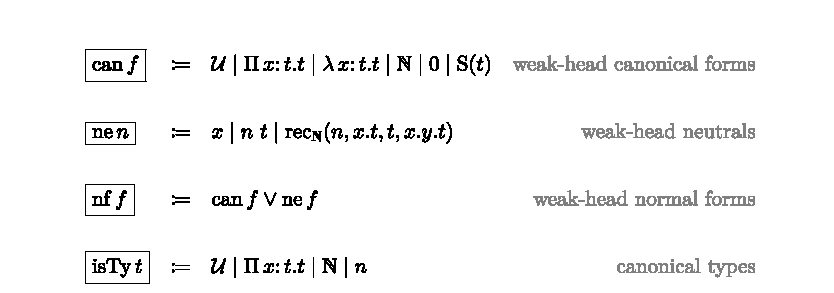
\includegraphics[width=0.98\linewidth,height=0.72\textheight,keepaspectratio]{rules-01.pdf}\end{center}
 
Figure 2:   Canonical, neutral, and normal form predicates (excerpt, see [34]). Way to read the BNF-style grammars: $\operatorname{isTy}$ is the predicate on terms given by the grammar $\operatorname{\mathcal{U}}\mid\operatorname{\Pi}x:t.t\mid\operatorname{\mathbb%
{N}}\mid n$ ($n$ stands for a neutral and $t$ for an arbitrary term).\par
 
% END S2.F2
 
% END S2.SS1.SSS0.P0.SPx1
 
% BEGIN S2.SS1.SSS0.P0.SPx2
 
\par\medskip\noindent\textbf{Normal forms and reduction.}\par
 
% BEGIN S2.SS1.SSS0.P0.SPx2.p1
 
Amongst terms, we particularly focus on (weak-head) normal forms, as this is the class with good injectivity properties, defined in Fig. 2. Canonical forms are terms starting with a constructor: $\operatorname{S}$, $\operatorname{\lambda}$, etc. Neutral forms are “stuck” terms, consisting of a spine of eliminators on top of a variable. Normal forms are either. We also define subclasses for each type: $\operatorname{isFun}t$ holds if $t$ is either a neutral or a $\operatorname{\lambda}$-abstraction, and similarly for $\operatorname{isTy}$ and $\operatorname{isNat}$. The $\operatorname{isTy_{+}}$ predicate isolates positive types: $\operatorname{\mathbb{N}}$, $\operatorname{\mathcal{U}}$ and neutrals.\par
 
% END S2.SS1.SSS0.P0.SPx2.p1
 
% BEGIN S2.F3

\begin{center}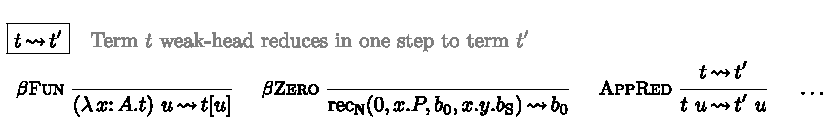
\includegraphics[width=0.98\linewidth,height=0.72\textheight,keepaspectratio]{rules-02.pdf}\end{center}
 
Figure 3:   Weak-head reduction (excerpt, see [34]).\par
 
% END S2.F3
 
% BEGIN S2.SS1.SSS0.P0.SPx2.p2
 
Finally, reduction $t\operatorname{\operatorname{\rightsquigarrow}^{\star}}t^{\prime}$ is the reflexive, transitive closure of one-step reduction, defined in Fig. 3. We use only a deterministic weak-head reduction. Reduction is not part of the specification of typing, we present it at this stage only to state normalisation in Sec. 2.2.\par
 
% END S2.SS1.SSS0.P0.SPx2.p2
 
% END S2.SS1.SSS0.P0.SPx2
 
% END S2.SS1
 
% BEGIN S2.SS2
 
\par\medskip\noindent\textbf{2.2 Meta-theory}\par
 
% BEGIN S2.SS2.p1
 
Let us now state the main meta-theoretic properties we consider – we comment about how to prove them at the end of this section and in Sec. 5. In Rocq, these are represented as type-classes: most theorems take instances of the relevant type-classes as parameters. This enables fine-grained bookkeeping of the theorems’ dependency, while keeping it lightweight as instances are automatically filled in. This is inspired by the treatment of function extensionality and univalence in the HoTT library [11].\par
 
% END S2.SS2.p1
 
% BEGIN S2.SS2.SSS0.P0.SPx1
 
\par\medskip\noindent\textbf{Type-level injectivity.}\par
 
% BEGIN Thmtheorem1
 
\par\medskip\noindent\textbf{Property 1 (  Injectivity and no-confusion of type constructors).}\par
 
% BEGIN Thmtheorem1.p1
 
Assume $T$ and $T^{\prime}$ are convertible types in weak-head normal form, i.e. we have that $\operatorname{isTy}T$, $\operatorname{isTy}T^{\prime}$, and $\Gamma\vdash T\mathrel{\raisebox{-0.5pt}{$\cong$}}T^{\prime}$. Then one of the following holds:\par
  
\par\noindent  $\blacksquare$ 
% BEGIN S2.I1.i1.p1
 
$T=\operatorname{\mathbb{N}}=T^{\prime}$ or $T=\operatorname{\mathcal{U}}=T^{\prime}$;\par
 
% END S2.I1.i1.p1
 
 
\par\noindent  $\blacksquare$ 
% BEGIN S2.I1.i2.p1
 
$T=\operatorname{\Pi}x:A.B$, $T^{\prime}=\operatorname{\Pi}x:A^{\prime}.B^{\prime}$, with $\Gamma\vdash A^{\prime}\mathrel{\raisebox{-0.5pt}{$\cong$}}A$ and $\Gamma,x:A^{\prime}\vdash B\mathrel{\raisebox{-0.5pt}{$\cong$}}B^{\prime}$;\par
 
% END S2.I1.i2.p1
 
 
\par\noindent  $\blacksquare$ 
% BEGIN S2.I1.i3.p1
 
$T$, $T^{\prime}$ are both neutral, and $\Gamma\vdash T\mathrel{\raisebox{-0.5pt}{$\cong$}}T^{\prime}\operatorname{%
\mathrel{:}}\operatorname{\mathcal{U}}$.\par
 
% END S2.I1.i3.p1
 
  
Any other case is thus impossible (no-confusion), e.g. we cannot have $\Gamma\vdash\operatorname{\Pi}x:A.B\mathrel{\raisebox{-0.5pt}{$\cong$}}%
\operatorname{\mathbb{N}}$.\par
 
% END Thmtheorem1.p1
 
% END Thmtheorem1
 
% BEGIN S2.SS2.SSS0.P0.SPx1.p1
 
This cannot be proven by mere induction, and indeed it implies a form of non-degeneracy, namely equational consistency: not all types are convertible. Consequences are numerous.\par
 
% END S2.SS2.SSS0.P0.SPx1.p1
 
% BEGIN Thmtheorem2
 
\par\medskip\noindent\textbf{Corollary 2 (  Preservation).}\par
 
% BEGIN Thmtheorem2.p1
 
Assuming Property 1, if $\Gamma\vdash A$ and $A\operatorname{\operatorname{\rightsquigarrow}^{\star}}A^{\prime}$ then $\Gamma\vdash A\mathrel{\raisebox{-0.5pt}{$\cong$}}A^{\prime}$. Similarly, if $\Gamma\vdash t\operatorname{\mathrel{:}}A$ and $t\operatorname{\operatorname{\rightsquigarrow}^{\star}}t^{\prime}$ then $\Gamma\vdash t\mathrel{\raisebox{-0.5pt}{$\cong$}}t^{\prime}\operatorname{%
\mathrel{:}}A$.\par
 
% END Thmtheorem2.p1
 
% END Thmtheorem2
 
% BEGIN Thmtheorem3
 
\par\medskip\noindent\textbf{Corollary 3 (  Types classify normal forms).}\par
 
% BEGIN Thmtheorem3.p1
 
Assuming Property 1, consider $t$ a normal form. If $\Gamma\vdash t\operatorname{\mathrel{:}}\operatorname{\Pi}x:A.B$, then $\operatorname{isFun}t$. If $\Gamma\vdash t\operatorname{\mathrel{:}}\operatorname{\mathbb{N}}$, then $\operatorname{isNat}t$. If $\Gamma\vdash t\operatorname{\mathrel{:}}\operatorname{\mathcal{U}}$, then $\operatorname{isTy}t$. If $\Gamma\vdash t\operatorname{\mathrel{:}}T$ and $T$ is neutral, then $t$ is neutral.\par
 
% END Thmtheorem3.p1
 
% END Thmtheorem3
 
% BEGIN S2.SS2.SSS0.P0.SPx1.p2
 
Preservation relies on the injectivity part, while classification uses no-confusion. Corollary 3 is the key lemma towards progress – the fact that every well-typed term is either a normal form or reduces –, although we do not show this in the formalisation. Thus, Property 1 suffices to establish safety in the progress-and-preservation approach [54].\par
 
% END S2.SS2.SSS0.P0.SPx1.p2
 
% END S2.SS2.SSS0.P0.SPx1
 
% BEGIN S2.SS2.SSS0.P0.SPx2
 
\par\medskip\noindent\textbf{Term-level injectivities.}\par
 
% BEGIN S2.SS2.SSS0.P0.SPx2.p1
 
Statements of injectivity (and no-confusion) for term constructors are relatively close to those for types.\par
 
% END S2.SS2.SSS0.P0.SPx2.p1
 
% BEGIN Thmtheorem4
 
\par\medskip\noindent\textbf{Property 4 (  Injectivity and no-confusion at $\operatorname{\mathbb{N}}$).}\par
 
% BEGIN Thmtheorem4.p1
 
Assume $n$ and $n^{\prime}$ are such that $\operatorname{isNat}n$, $\operatorname{isNat}n^{\prime}$, and $\Gamma\vdash n\mathrel{\raisebox{-0.5pt}{$\cong$}}n^{\prime}\operatorname{%
\mathrel{:}}\operatorname{\mathbb{N}}$. Then one of the following must hold:\par
  
\par\noindent  $\blacksquare$ 
% BEGIN S2.I2.i1.p1
 
$n=0=n^{\prime}$;\par
 
% END S2.I2.i1.p1
 
 
\par\noindent  $\blacksquare$ 
% BEGIN S2.I2.i2.p1
 
$n=\operatorname{S}(t)$, $n^{\prime}=\operatorname{S}(t^{\prime})$, with $\Gamma\vdash t\mathrel{\raisebox{-0.5pt}{$\cong$}}t^{\prime}\operatorname{%
\mathrel{:}}\operatorname{\mathbb{N}}$;\par
 
% END S2.I2.i2.p1
 
 
\par\noindent  $\blacksquare$ 
% BEGIN S2.I2.i3.p1
 
$n$, $n^{\prime}$ are both neutral.\par
 
% END S2.I2.i3.p1
 
  
% END Thmtheorem4.p1
 
% END Thmtheorem4
 
% BEGIN S2.SS2.SSS0.P0.SPx2.p2
 
Maybe surprisingly, the eliminator makes these statements directly provable. Indeed, assuming $\operatorname{S}(t)\mathrel{\raisebox{-0.5pt}{$\cong$}}\operatorname{S}(t^{%
\prime})$, by the computation and congruence rule for the eliminator, we get that $t\mathrel{\raisebox{-0.5pt}{$\cong$}}\operatorname{rec}_{\operatorname{\mathbb%
{N}}}(x.\operatorname{\mathbb{N}},\operatorname{S}(t),0,x.y.x)\mathrel{%
\raisebox{-0.5pt}{$\cong$}}\operatorname{rec}_{\operatorname{\mathbb{N}}}(x.%
\operatorname{\mathbb{N}},\operatorname{S}(t^{\prime}),0,x.y.x)\mathrel{%
\raisebox{-0.5pt}{$\cong$}}t^{\prime}\operatorname{\mathrel{:}}\operatorname{%
\mathbb{N}}$. We can similarly reduce no-confusion to that for types. A similar phenomenon happens at $\operatorname{\Pi}$ types, where injectivity of $\operatorname{\lambda}$ can also be directly derived.\par
 
% END S2.SS2.SSS0.P0.SPx2.p2
 
% BEGIN S2.SS2.SSS0.P0.SPx2.p3
 
Injectivity for the universe ( ) follows a similar pattern, but is not so easily proven for lack of an eliminator. For neutral types, which have no constructors, Corollary 3 is all we need: two (convertible) normal forms at a neutral type must be neutrals.\par
 
% END S2.SS2.SSS0.P0.SPx2.p3
 
% END S2.SS2.SSS0.P0.SPx2
 
% BEGIN S2.SS2.SSS0.P0.SPx3
 
\par\medskip\noindent\textbf{Neutral injectivities.}\par
 
% BEGIN S2.SS2.SSS0.P0.SPx3.p1
 
To complete the injectivity picture, we turn to neutrals, for which injectivity/no-confusion can be expressed in two ways. The first follows a familiar pattern.\par
 
% END S2.SS2.SSS0.P0.SPx3.p1
 
% BEGIN Thmtheorem5
 
\par\medskip\noindent\textbf{Property 5 (  Injectivity of neutral eliminators).}\par
 
% BEGIN Thmtheorem5.p1
 
Assume $n$ and $n^{\prime}$ are neutrals such that $\Gamma\vdash n\mathrel{\raisebox{-0.5pt}{$\cong$}}n^{\prime}\operatorname{%
\mathrel{:}}T$. Then one of the following must hold:\par
  
\par\noindent  $\blacksquare$ 
% BEGIN S2.I3.i1.p1
 
$n=x=n^{\prime}$, with $(x:T^{\prime})\in\Gamma$ and $\Gamma\vdash T^{\prime}\mathrel{\raisebox{-0.5pt}{$\cong$}}T$;\par
 
% END S2.I3.i1.p1
 
 
\par\noindent  $\blacksquare$ 
% BEGIN S2.I3.i2.p1
 
$n=m\ u$, $n^{\prime}=m^{\prime}\ u^{\prime}$ with $\Gamma\vdash m\mathrel{\raisebox{-0.5pt}{$\cong$}}m^{\prime}\operatorname{%
\mathrel{:}}\operatorname{\Pi}x:A.B$, $\Gamma\vdash u\mathrel{\raisebox{-0.5pt}{$\cong$}}u^{\prime}\operatorname{%
\mathrel{:}}A$ and $\Gamma\vdash B\mathord{\left[u\right]}\mathrel{\raisebox{-0.5pt}{$\cong$}}T$;\par
 
% END S2.I3.i2.p1
 
 
\par\noindent  $\blacksquare$ 
% BEGIN S2.I3.i3.p1
 
$n=\operatorname{rec}_{\operatorname{\mathbb{N}}}(m,x.P,t_{0},x.y.t_{%
\operatorname{S}})$, $n^{\prime}=\operatorname{rec}_{\operatorname{\mathbb{N}}}(m^{\prime},x.P^{%
\prime},t^{\prime}_{0},x.y.t^{\prime}_{\operatorname{S}})$, with convertible subterms.\par
 
% END S2.I3.i3.p1
 
  
% END Thmtheorem5.p1
 
% END Thmtheorem5
 
% BEGIN S2.SS2.SSS0.P0.SPx3.p2
 
However, in some cases this is too strong: at negative types our type-directed algorithm eagerly $\eta$-expands, so the above are only really needed at positive types. To state the “minimal” property we require, we take another way, starting with the following definition.\par
 
% END S2.SS2.SSS0.P0.SPx3.p2
 
% BEGIN Thmtheorem6
 
\par\medskip\noindent\textbf{Definition 6 (  Neutral comparison).}\par
 
% BEGIN Thmtheorem6.p1
 
Neutral comparison (see Sec. A.2), written $\Gamma\vdash n\sim n^{\prime}\operatorname{\mathrel{:}}T$, is the least relation that is:\par
  
\par\noindent  $\blacksquare$ 
% BEGIN S2.I4.i1.p1
 
reflexive on variables, i.e. $\Gamma\vdash x\sim x\operatorname{\mathrel{:}}T$ if $(x:T)\in\Gamma$;\par
 
% END S2.I4.i1.p1
 
 
\par\noindent  $\blacksquare$ 
% BEGIN S2.I4.i2.p1
 
closed under the congruence rules for eliminators;\par
 
% END S2.I4.i2.p1
 
 
\par\noindent  $\blacksquare$ 
% BEGIN S2.I4.i3.p1
 
stable under conversion: if $\Gamma\vdash n\sim n^{\prime}\operatorname{\mathrel{:}}T$ and $\Gamma\vdash T\mathrel{\raisebox{-0.5pt}{$\cong$}}T^{\prime}$ then $\Gamma\vdash n\sim n^{\prime}\operatorname{\mathrel{:}}T^{\prime}$.\par
 
% END S2.I4.i3.p1
 
  
% END Thmtheorem6.p1
 
% END Thmtheorem6
 
% BEGIN S2.SS2.SSS0.P0.SPx3.p3
 
We can then rephrase injectivity of neutral constructors as follows.\par
 
% END S2.SS2.SSS0.P0.SPx3.p3
 
% BEGIN Thmtheorem7
 
\par\medskip\noindent\textbf{Property 7 (  Completeness of neutral comparison).}\par
 
% BEGIN Thmtheorem7.p1
 
Given any two neutrals $n$ and $n^{\prime}$ such that $\Gamma\vdash n\mathrel{\raisebox{-0.5pt}{$\cong$}}n^{\prime}\operatorname{%
\mathrel{:}}T$, we have $\Gamma\vdash n\sim n^{\prime}\operatorname{\mathrel{:}}T$.\par
 
% END Thmtheorem7.p1
 
% END Thmtheorem7
 
% BEGIN Thmtheorem8
 
\par\medskip\noindent\textbf{Proposition 8 ( ).}\par
 
% BEGIN Thmtheorem8.p1
 
Property 5 and Property 7 are equivalent.\par
 
% END Thmtheorem8.p1
 
% END Thmtheorem8
 
% BEGIN S2.SS2.SSS0.P0.SPx3.p4
 
But now, we can weaken it to only consider positive types.\par
 
% END S2.SS2.SSS0.P0.SPx3.p4
 
% BEGIN Thmtheorem9
 
\par\medskip\noindent\textbf{Property 9 (  Completeness of neutral comparison at positive types).}\par
 
% BEGIN Thmtheorem9.p1
 
Given any two neutrals $n$ and $n^{\prime}$ such that $\Gamma\vdash n\mathrel{\raisebox{-0.5pt}{$\cong$}}n^{\prime}\operatorname{%
\mathrel{:}}T$, if moreover $\operatorname{isTy_{+}}T$, then we have $\Gamma\vdash n\sim n^{\prime}\operatorname{\mathrel{:}}T$.\par
 
% END Thmtheorem9.p1
 
% END Thmtheorem9
 
% END S2.SS2.SSS0.P0.SPx3
 
% BEGIN S2.SS2.SSS0.P0.SPx4
 
\par\medskip\noindent\textbf{Normalisation.}\par
 
% BEGIN S2.SS2.SSS0.P0.SPx4.p1
 
The last property is normalisation. Its main use is to argue for termination of the algorithm, so it has to go beyond weak-head reduction and take into account $\eta$-expansion, and subterms of (weak-head) normal forms.\par
 
% END S2.SS2.SSS0.P0.SPx4.p1
 
% BEGIN Thmtheorem10
 
\par\medskip\noindent\textbf{Definition 10 (  Deeply normalising).}\par
 
% BEGIN Thmtheorem10.p1
 
A term $t$ is deeply normalising at type $A$ in context $\Gamma$ if they reduce respectively to weak-head normal forms $t^{\prime}$ and $A^{\prime}$, and moreover:\par
  
\par\noindent  $\blacksquare$ 
% BEGIN S2.I5.i1.p1
 
$A^{\prime}$ is a negative type, and the $\eta$-expansion of $t^{\prime}$ is itself normalising;\par
 
% END S2.I5.i1.p1
 
 
\par\noindent  $\blacksquare$ 
% BEGIN S2.I5.i2.p1
 
or $A^{\prime}$ is a positive type, and the subterms of $t^{\prime}$ are normalising at the relevant types.\par
 
% END S2.I5.i2.p1
 
  
A type $A$ is deeply normalising in context $\Gamma$ if it reduces to a weak-head normal form, whose subterms are themselves normalising. See [34] for the inference rules.\par
 
% END Thmtheorem10.p1
 
% END Thmtheorem10
 
% BEGIN S2.SS2.SSS0.P0.SPx4.p2
 
While not apparent in this short version of the definition, the context actually plays a role in order to express the type at which a neutral should be normalising.\par
 
% END S2.SS2.SSS0.P0.SPx4.p2
 
% BEGIN Thmtheorem11
 
\par\medskip\noindent\textbf{Property 11 (  Deep normalisation).}\par
 
% BEGIN Thmtheorem11.p1
 
Every well-typed term is deeply normalising (at its type). Every well-formed type is deeply normalising.\par
 
% END Thmtheorem11.p1
 
% END Thmtheorem11
 
% BEGIN S2.SS2.SSS0.P0.SPx4.p3
 
Meta-theoretic consequences include canonicity ( ) – any closed term of type $\operatorname{\mathbb{N}}$ is convertible to one of the form $\operatorname{S}^{n}0$ – and, most importantly, logical consistency. This means that to prove Property 11, the meta-theory must be logically stronger than the object theory.\par
 
% END S2.SS2.SSS0.P0.SPx4.p3
 
% BEGIN Thmtheorem12
 
\par\medskip\noindent\textbf{Corollary 12 (  Logical consistency).}\par
 
% BEGIN Thmtheorem12.p1
 
Assuming Property 11, there are no closed terms of type $\operatorname{\bot}$.\par
 
% END Thmtheorem12.p1
 
% END Thmtheorem12
 
% END S2.SS2.SSS0.P0.SPx4
 
% BEGIN S2.SS2.SSS0.P0.SPx5
 
\par\medskip\noindent\textbf{Proving the properties.}\par
 
% BEGIN S2.SS2.SSS0.P0.SPx5.p1
 
In our formalisation, most properties are proven via a logical relation, in the style pioneered by Abel et al. [3], and later adapted in Rocq [7], to which we refer for details. Multiple universes in the meta-theory provide the logical strength we need to prove consistency. This approach is however by far not the only possibility, see the discussion in Sec. 5. Note the following two points.\par
 
% END S2.SS2.SSS0.P0.SPx5.p1
 
% BEGIN S2.SS2.SSS0.P0.SPx5.p2
 
First, the proof of deep normalisation is indirect. Indeed, the logical relation is parameterised by an abstract partial equivalence relation (PER) relating neutrals, which we instantiate with algorithmic neutral comparison to obtain normalisation for subterms of neutrals. To avoid this detour through algorithmic aspects, we envisioned strengthening the logical relation to directly encompass neutrals, but did not find a satisfying approach.\par
 
% END S2.SS2.SSS0.P0.SPx5.p2
 
% BEGIN S2.SS2.SSS0.P0.SPx5.p3
 
Second, as logical relations at negative types are naturally defined by observations (e.g. a function is reducible when its application to reducible inputs are reducible), these types “know nothing” about neutrals, and completeness of neutral comparison at negative types cannot be derived easily. We expect other proofs of “semantic” flavour to have similar issues with full completeness of neutrals, making the restriction to positive types (Property 9 vs. Property 7) an important distinction. And indeed, while completeness at positive types is a direct consequence of our logical relation ( ), the approach we found to completeness at all types takes a long detour via the two algorithmic presentations ( ) and strengthening.\par
 
% END S2.SS2.SSS0.P0.SPx5.p3
 
% END S2.SS2.SSS0.P0.SPx5
 
% END S2.SS2
 
% END S2


% BEGIN S3
 
\par\medskip\noindent\textbf{3 Algorithmic typing and conversion}\par
 
% BEGIN S3.p1
 
Let us now turn to our algorithms for conversion and typing. Only the untyped conversion algorithm is new, the typed conversion and bidirectional typing ones come directly from MLTT à la Coq [7]. We give the algorithms informally as rules, which are translated in the formalisation in two ways. First ( ) as inductively defined relations, like declarative typing. Second, we implement them as functions ( ). As we wish to separate their definition from their termination argument, we must embrace partiality. To that end, we use McBride’s free recursion monad [41], via Winterhalter’s PartialFun [53]. This lets us define the functions prior to any proofs; immediately execute them with bounded recursion depth – McBride’s “petrol semantics”; extract a typing (dis)proof from a terminating execution once we prove either soundness; and get proper decidability once we show normalisation. Cherry on the cake: as the recursion monad exposes the programs’ recursive structure, we can generically derive “functional” induction principles, following said recursive structures.\par
 
% END S3.p1
 
% BEGIN S3.SS0.SSS0.P0.SPx1
 
\par\medskip\noindent\textbf{Bidirectional typing.}\par
 
% BEGIN S3.SS0.SSS0.P0.SPx1.p1
 
Our typing algorithm, as most for dependent types, is bidirectional: it separates inference, written $\Gamma\vdash t\mathrel{\rhd}T$, where the type is an output to be found, from type checking, written $\Gamma\vdash t\operatorname{\mathrel{\lhd}}T$, where the type is a constraint given as input. We refer to others [42, 20, 31] for exposition – this last reference is the closest to us. Bidirectional typing generally has two main interests, although only the first is relevant to us here.\par
 
% END S3.SS0.SSS0.P0.SPx1.p1
 
% BEGIN S3.SS0.SSS0.P0.SPx1.p2
 
First, bidirectional typing gives better control over conversion. By replacing the conversion rule with syntax-directed rules, we get a term-directed system, amenable to implementation. This makes the bidirectional system a priori more restrictive than the declarative one, since we have strictly constrained the way conversion can be used. The main point of negative soundness is to show that this restriction does not, in fact, lose anything.\par
 
% END S3.SS0.SSS0.P0.SPx1.p2
 
% BEGIN S3.SS0.SSS0.P0.SPx1.p3
 
Second, propagating types “up” in derivations lightens the need for type annotations and gives better error messages. This is important for surface languages, less for kernels, where terms are typically not human-written. On the contrary, extra information can be useful in various ways, and we would rather dispense of the complication of segregating terms containing too little information to infer. Hence, as Rocq and Lean, we adopt a syntax where all terms infer, although completeness for the other approach is certainly interesting and feasible [35].\par
 
% END S3.SS0.SSS0.P0.SPx1.p3
 
% BEGIN S3.F4

\begin{center}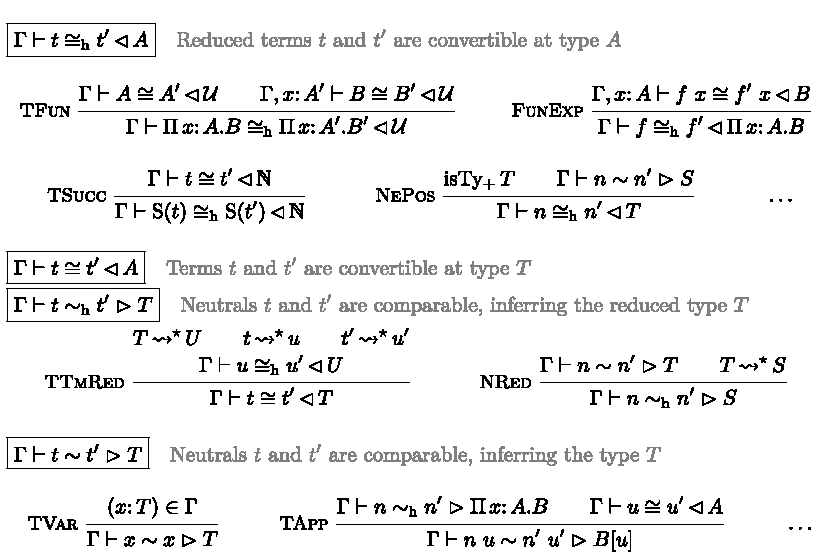
\includegraphics[width=0.98\linewidth,height=0.72\textheight,keepaspectratio]{rules-03.pdf}\end{center}
 
Figure 4:   Typed conversion algorithm (excerpt, see Sec. B.1).\par
 
% END S3.F4
 
% END S3.SS0.SSS0.P0.SPx1
 
% BEGIN S3.SS0.SSS0.P0.SPx2
 
\par\medskip\noindent\textbf{Typed conversion is bidirectional.}\par
 
% BEGIN S3.SS0.SSS0.P0.SPx2.p1
 
A point already implicitly present in Abel et al. [3], but made explicit in Adjedj et al. [7], is that the type-directed conversion algorithm is bidirectional, too. It is decomposed in two main functions, one to compare general terms and the other dedicated to neutrals. The former takes a type as input – it is checking –, while the latter reconstructs types as it traverses the neutrals – it is inferring.\par
 
% END S3.SS0.SSS0.P0.SPx2.p1
 
% BEGIN S3.SS0.SSS0.P0.SPx2.p2
 
More precisely, conversion (see Fig. 4), written $\Gamma\vdash t\mathrel{\raisebox{-0.5pt}{$\cong$}}u\operatorname{\mathrel{\lhd%
}}A$, goes as follows:\par
  
\par\noindent  1. 
% BEGIN S3.I1.i1.p1
 
reduce $t$, $u$ and $A$ to weak-head normal forms;\par
 
% END S3.I1.i1.p1
 
 
\par\noindent  2. 
% BEGIN S3.I1.i2.p1
 
if $A$ is a negative type ($\operatorname{\Pi},\operatorname{\Sigma}$), recursively compare the $\eta$-expansions of $t$ and $u$;\par
 
% END S3.I1.i2.p1
 
 
\par\noindent  3. 
% BEGIN S3.I1.i3.p1
 
if $A$ is a positive type ($\operatorname{\mathbb{N}},\operatorname{\mathcal{U}},\dots$) and the terms are canonical, use the relevant congruence;\par
 
% END S3.I1.i3.p1
 
 
\par\noindent  4. 
% BEGIN S3.I1.i4.p1
 
if $A$ is a positive type and the terms are neutrals, call neutral comparison.\par
 
% END S3.I1.i4.p1
 
  
Steps 2-4 are delegated to an auxiliary function, denoted $\mathrel{\raisebox{-0.5pt}{$\cong$}}_{\mathrm{h}}$ (the “h” is for “head”). Neutral comparison, written $\Gamma\vdash n\sim n^{\prime}\mathrel{\rhd}S$ follows their structure, applying congruences as it goes.\par
 
% END S3.SS0.SSS0.P0.SPx2.p2
 
% BEGIN S3.SS0.SSS0.P0.SPx2.p3
 
Rule   Typed conversion algorithm (excerpt, see Sec.˜B.1). demonstrates this bidirectional yoga. As conversion is type-directed, we need a type $A$ to compare the arguments, that is obtained through the recursive comparison of the functions, which must thus be inferring. We would not be able to construct $\operatorname{\Pi}x:A.B$ anyway, even given $B\mathord{\left[u\right]}$: inverting substitutions is unfeasible. Thus, even with a syntax with complete inference, the distinction between checking constructors and inferring eliminators, a landmark of the “Nordic” approach to bidirectionalism [43, 42], appears naturally.\par
 
% END S3.SS0.SSS0.P0.SPx2.p3
 
% END S3.SS0.SSS0.P0.SPx2
 
% BEGIN S3.SS0.SSS0.P0.SPx3
 
\par\medskip\noindent\textbf{Untyped conversion.}\par
 
% BEGIN S3.F5

\begin{center}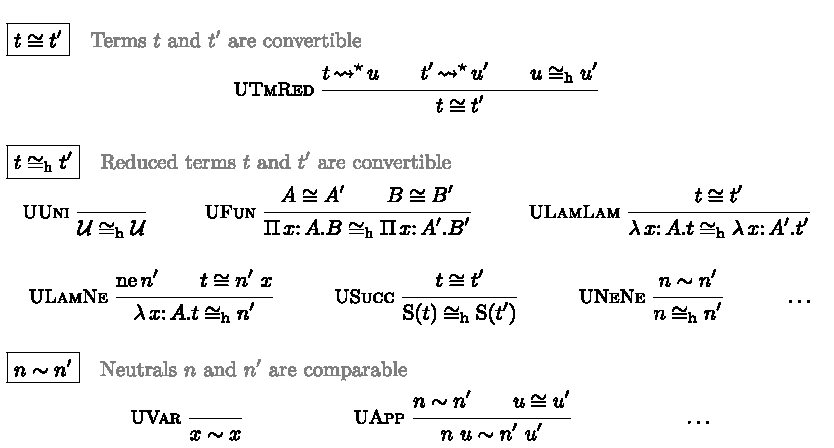
\includegraphics[width=0.98\linewidth,height=0.72\textheight,keepaspectratio]{rules-04.pdf}\end{center}
 
Figure 5:   Untyped algorithmic conversion (excerpt, see Sec. B.2).\par
 
% END S3.F5
 
% BEGIN S3.SS0.SSS0.P0.SPx3.p1
 
Untyped conversion (Fig. 5) looks much simpler than typed conversion: there are no types, no separation between type and term conversion, and the separation of neutral comparison is kept mostly for readability.\par
 
% END S3.SS0.SSS0.P0.SPx3.p1
 
% BEGIN S3.SS0.SSS0.P0.SPx3.p2
 
The main point is that we replace the all-encompassing   Typed conversion algorithm (excerpt, see Sec.˜B.1). by term-directed rules, an approach pioneered by Coquand, first for functions [16], then pairs [2]. When comparing $\operatorname{\lambda}$-abstractions, we apply the congruence   Untyped algorithmic conversion (excerpt, see Sec.˜B.2). – which would also happen in   Typed conversion algorithm (excerpt, see Sec.˜B.1). after contracting the redexes. If one side is a $\operatorname{\lambda}$ and the other a neutral (  Untyped algorithmic conversion (excerpt, see Sec.˜B.2).), we again simulate   Typed conversion algorithm (excerpt, see Sec.˜B.1)., but this time we see the application to a fresh variable is visible on the neutral’s side. And this is all! That is, there is no $\eta$-rule when the two sides are neutrals. How could there be? In the extreme case of two variables, the only information we could use is… type information, which we precisely decided not to rely on. This discrepancy on neutrals at negative types is the key difference between the two algorithms.\par
 
% END S3.SS0.SSS0.P0.SPx3.p2
 
% END S3.SS0.SSS0.P0.SPx3
 
% BEGIN S3.SS0.SSS0.P0.SPx4
 
\par\medskip\noindent\textbf{Comparison.}\par
 
% BEGIN S3.SS0.SSS0.P0.SPx4.p1
 
As a concrete example, we can look at the “execution trace” in the following problem: $x:\operatorname{\mathbb{N}}\to\operatorname{\mathbb{N}}\vdash x\mathrel{%
\raisebox{-0.5pt}{$\cong$}}x\operatorname{\mathrel{:}}\operatorname{\mathbb{N}%
}\to\operatorname{\mathbb{N}}$. The untyped algorithm immediately uses   Untyped algorithmic conversion (excerpt, see Sec.˜B.2). to go in “neutral mode”, and finishes with   Untyped algorithmic conversion (excerpt, see Sec.˜B.2).. The typed algorithm, on the other hand, first $\eta$-expands, introducing a fresh variable $y$, and recursively compares $x\ y$ to $x\ y$. Only then, by reaching a positive type, does it change to “neutral mode”. Neutral comparison then peels off the application node, compares $x$ to $x$ again but this time as neutrals, and finally applies variable reflexivity. It also needs to compare $y$ to $y$ first as normal forms at $\operatorname{\mathbb{N}}$, then as neutrals, and finally terminates. We can already see the work spared by the term-directed algorithm – exacerbated for $\operatorname{\Sigma}$ types, where $\eta$ introduces duplication.\par
 
% END S3.SS0.SSS0.P0.SPx4.p1
 
% END S3.SS0.SSS0.P0.SPx4
 
% END S3


% BEGIN S4.SS1
 
\par\medskip\noindent\textbf{4.1 Properties of typed conversion}\par
 
% BEGIN S4.SS1.p1
 
Most results in this section are not per se new, although they were significantly reworked, in particular to precisely track their dependencies. In particular, termination relies explicitly on normalisation, rather than on the reflexivity of the logical relation. The work around negative soundness is entirely new.\par
 
% END S4.SS1.p1
 
% BEGIN S4.SS1.SSS0.P0.SPx1
 
\par\medskip\noindent\textbf{Positive soundness.}\par
 
% BEGIN S4.SS1.SSS0.P0.SPx1.p1
 
We split the proof in two, using the inductive judgment as intermediate. The first half is almost tautological, and does not depend on any meta-theory.\par
 
% END S4.SS1.SSS0.P0.SPx1.p1
 
% BEGIN Thmtheorem13
 
\par\medskip\noindent\textbf{Proposition 13 (  Positive soundness of the typed conversion function).}\par
 
% BEGIN Thmtheorem13.p1
 
If a typed conversion function returns a positive answer, then the corresponding judgment of Fig. 4 holds.\par
 
% END Thmtheorem13.p1
 
% END Thmtheorem13
 
% BEGIN Thmtheorem14
 
\par\medskip\noindent\textbf{Proposition 14 (  Positive soundness of the typed algorithmic conversion judgment).}\par
 
% BEGIN Thmtheorem14.p1
 
Assuming injectivity of type constructors (Property 1), the algorithmic typed conversion judgments imply their postconditions whenever their preconditions hold.\par
 
% END Thmtheorem14.p1
 
% END Thmtheorem14
 
% BEGIN S4.SS1.SSS0.P0.SPx1.p2
 
This second half is the interesting one. The crucial part of this proof, and the backbone of others in this section, is to show that each inductive rule correctly preserves the invariants. This is a very regular property, so much that we meta-programmed444 We hardcoded these in the current code to remove a dependency which caused proof engineering issues.  the generation of “local preservation lemmas” ( ) for each rule, expressing this idea. We assemble these lemmas into a “bundled induction principle”, again programmatically generated, which threads the invariants through, giving access to them as extra hypotheses in each induction step. Soundness follows by instantiating this induction principle with the constant True predicates.\par
 
% END S4.SS1.SSS0.P0.SPx1.p2
 
% END S4.SS1.SSS0.P0.SPx1
 
% BEGIN S4.SS1.SSS0.P0.SPx2
 
\par\medskip\noindent\textbf{Negative soundness.}\par
 
% BEGIN S4.SS1.SSS0.P0.SPx2.p1
 
For negative soundness, we cannot go through the intermediate algorithmic judgments, as they only encode successful runs of the functions. Thus, we bite the bullet and directly relate the output of the functions to the declarative judgments.\par
 
% END S4.SS1.SSS0.P0.SPx2.p1
 
% BEGIN Thmtheorem15
 
\par\medskip\noindent\textbf{Proposition 15 (  Negative soundness of typed algorithmic conversion).}\par
 
% BEGIN Thmtheorem15.p1
 
Assuming injectivity of type and term constructors (Properties 1, 4, etc.), and completeness of neutral conversion at positive types (Property 9), if a typed conversion function returns a negative answer and its precondition holds, then its postcondition cannot hold.\par
 
% END Thmtheorem15.p1
 
% END Thmtheorem15
 
% BEGIN S4.SS1.SSS0.P0.SPx2.p2
 
Again, we rely on invariant preservation, the proof is otherwise straightforward: we have extracted exactly the injectivity properties needed to justify each step. In essence, we show that at any stage the current “remaining goals” are equivalent to the initial query, relying on injectivity to know that we only use invertible congruences, which are safe to apply.\par
 
% END S4.SS1.SSS0.P0.SPx2.p2
 
% END S4.SS1.SSS0.P0.SPx2
 
% BEGIN S4.SS1.SSS0.P0.SPx3
 
\par\medskip\noindent\textbf{Termination.}\par
 
% BEGIN S4.SS1.SSS0.P0.SPx3.p1
 
As expected, this is where normalisation becomes necessary. As before, we need invariants throughout, and thus injectivity of type constructors. The most subtle part of the proof concerns the reduction machine.\par
 
% END S4.SS1.SSS0.P0.SPx3.p1
 
% BEGIN Thmtheorem16
 
\par\medskip\noindent\textbf{Lemma 16 (  Completeness of reduction).}\par
 
% BEGIN Thmtheorem16.p1
 
Assuming Property 1, if $t$ is well-typed and reduces to the weak-head normal form $t^{\prime}$, then the reduction function applied to $t$ returns $t^{\prime}$.\par
 
% END Thmtheorem16.p1
 
% END Thmtheorem16
 
% BEGIN S4.SS1.SSS0.P0.SPx3.p2
 
The main task is to define a well-founded order on the configurations of the abstract machine implementing reduction, a lexicographic product of subterm ordering and reduction. The assumption that $t$ reduces to a weak-head normal form ensures that this order is well-founded. Winterhalter introduced a similar order for MetaCoq [52, chap. 23].\par
 
% END S4.SS1.SSS0.P0.SPx3.p2
 
% BEGIN Thmtheorem17
 
\par\medskip\noindent\textbf{Proposition 17 (  Termination of typed algorithmic conversion).}\par
 
% BEGIN Thmtheorem17.p1
 
Assuming injectivity of type constructors (Property 1) and deep normalisation (Property 11), typed conversion functions terminate whenever their preconditions are satisfied.\par
 
% END Thmtheorem17.p1
 
% END Thmtheorem17
 
% BEGIN S4.SS1.SSS0.P0.SPx3.p3
 
The proof is by induction on deep normalisation, again using local preservation lemmas. The inductive structure of deep normalisation readily encodes the combination of subterm, reduction and $\eta$-expansion that one needs to be well-founded. In contrast, in MetaCoq, Winterhalter introduced a complex dependent lexicographic order modulo [52, chap 24], and admits that his setup would not easily incorporate $\eta$-expansion.\par
 
% END S4.SS1.SSS0.P0.SPx3.p3
 
% END S4.SS1.SSS0.P0.SPx3
 
% BEGIN S4.SS1.SSS0.P0.SPx4
 
\par\medskip\noindent\textbf{Non-triviality.}\par
 
% BEGIN S4.SS1.SSS0.P0.SPx4.p1
 
Soundness, both positive and negative, has a default: the nowhere-defined function is sound! Although we repeat that these properties should not be read to merely say “there exists a function such that…” but to characterise a particular checker – that we can run on examples ( ) to check for non-triviality –, it is good to formally ensure that our functions are non-trivial. Again, this is split in two.\par
 
% END S4.SS1.SSS0.P0.SPx4.p1
 
% BEGIN Thmtheorem18
 
\par\medskip\noindent\textbf{Proposition 18 (  Completeness of the implementation).}\par
 
% BEGIN Thmtheorem18.p1
 
Assuming injectivity of type constructors (Property 1), if an algorithmic conversion judgment and its precondition hold, then the corresponding function answers positively.\par
 
% END Thmtheorem18.p1
 
% END Thmtheorem18
 
% BEGIN S4.SS1.SSS0.P0.SPx4.p2
 
Next, we show that algorithmic conversion satisfies many closure properties, which Abel et al. call “generic conversion”. These are rather rich: all the proofs on the logical relation side can be done with respect to any generic conversion.\par
 
% END S4.SS1.SSS0.P0.SPx4.p2
 
% BEGIN Thmtheorem19
 
\par\medskip\noindent\textbf{Proposition 19 ( ).}\par
 
% BEGIN Thmtheorem19.p1
 
Algorithmic conversion is a generic conversion, thus for instance symmetric and transitive, stable by weakening and expansion, congruent for constructors.\par
 
% END Thmtheorem19.p1
 
% END Thmtheorem19
 
% BEGIN S4.SS1.SSS0.P0.SPx4.p3
 
Compared to declarative typing, the only missing part is congruences for eliminators, which only hold for neutral conversion, and reflexivity – which would be direct by induction if we had all congruence rules. The point is that eliminator congruences are the dangerous ones that can trigger reductions: applying a normal form to a normal form does not yield a normal form. And indeed a term is deeply normalising exactly when it is reflexive for (typed) algorithmic conversion, explaining why reflexivity cannot be achieved easily.\par
 
% END S4.SS1.SSS0.P0.SPx4.p3
 
% END S4.SS1.SSS0.P0.SPx4
 
% BEGIN S4.SS1.SSS0.P0.SPx5
 
\par\medskip\noindent\textbf{Typing.}\par
 
% BEGIN S4.SS1.SSS0.P0.SPx5.p1
 
All of these propositions extend to bidirectional typing. More precisely, assuming any conversion relation/function between types that satisfies the relevant property, we can derive a similar one for typing. This means that the proofs are modular, in that we can swap out a different implementation of conversion, as long as it satisfies the right properties, which is exactly what we are about to do.\par
 
% END S4.SS1.SSS0.P0.SPx5.p1
 
% END S4.SS1.SSS0.P0.SPx5
 
% END S4.SS1


% BEGIN S4.SS2
 
\par\medskip\noindent\textbf{4.2 Properties of untyped conversion}\par
 
% BEGIN S4.SS2.p1
 
The high-level ideas are very similar to typed conversion. For positive soundness there is really no difference: the equivalents of Propositions 13 ( ) and 14 ( ) hold. Even better, we can reuse most of the local preservation lemmas directly.\par
 
% END S4.SS2.p1
 
% BEGIN S4.SS2.p2
 
Negative soundness is where the subtle difference between the two algorithms shows. Echoing the discussion in Secs. 2.2 and 3, the key point is neutrals at negative types. And indeed, while in Proposition 15 we could make do with the weaker completeness (Property 9), this time we really need the full power of completeness at all types.\par
 
% END S4.SS2.p2
 
% BEGIN Thmtheorem20
 
\par\medskip\noindent\textbf{Proposition 20 (  Negative soundness of untyped algorithmic conversion).}\par
 
% BEGIN Thmtheorem20.p1
 
Assuming injectivity of type and term constructors (Properties 1, 4, etc.), and completeness of neutral conversion at all types (Property 7), if the untyped conversion function returns a negative answer and its preconditions holds, then its postcondition cannot hold.\par
 
% END Thmtheorem20.p1
 
% END Thmtheorem20
 
% BEGIN S4.SS2.p3
 
As for termination, there is a twist again, of course at negative types. The issue is that deep normalisation systematically $\eta$-expands terms, but untyped conversion does not always do this. Worse, it is non-deterministic, in the sense that whether a given term is $\eta$-expanded depends on the term it is compared to. Thus, our termination measure is not exactly fit, and circumventing the issue involves proving a form of strengthening of the algorithm: it gives the same output when irrelevant variables are removed from the context.\par
 
% END S4.SS2.p3
 
% BEGIN Thmtheorem21
 
\par\medskip\noindent\textbf{Proposition 21 (  Termination of untyped algorithmic conversion).}\par
 
% BEGIN Thmtheorem21.p1
 
Assuming Property 1 and Property 11, untyped conversion functions terminate whenever their preconditions hold.\par
 
% END Thmtheorem21.p1
 
% END Thmtheorem21
 
% END S4.SS2


% BEGIN S4.SS3
 
\par\medskip\noindent\textbf{4.3 Equivalence between the algorithms}\par
 
% BEGIN S4.SS3.p1
 
To wrap up, we can directly compare the two algorithms. Given how close they are, this should be rather easy, or at any rate easier than comparing declarative systems – where the seemingly innocuous transitivity is actually a source of headaches [44], because it means “real” untyped conversion can relate well-typed terms through ill-typed ones, which cannot be easily emulated by its typed counterpart. In fact, streamlining the relation between typed and untyped conversion was one of our original motivation [31, chap. 6] [32].\par
 
% END S4.SS3.p1

% BEGIN A1
 
\par\medskip\noindent\textbf{Appendix A Declarative Martin-Löf Type Theory}\par
 
% BEGIN A1.p1
 
On top of $t\mathord{\left[u\right]}$ for the substitution of the last variable of $t$ by $u$, we more generally use $t\mathord{\left[u,v,w\right]}$ for the parallel substitution of the last variables of $t$ with $u$, $v$ and $w$.\par
 
% END A1.p1
 
% BEGIN A1.SS1
 
\par\medskip\noindent\textbf{A.1 Declarative conversion}\par
 
% BEGIN A1.SS1.p1
 
\begin{center}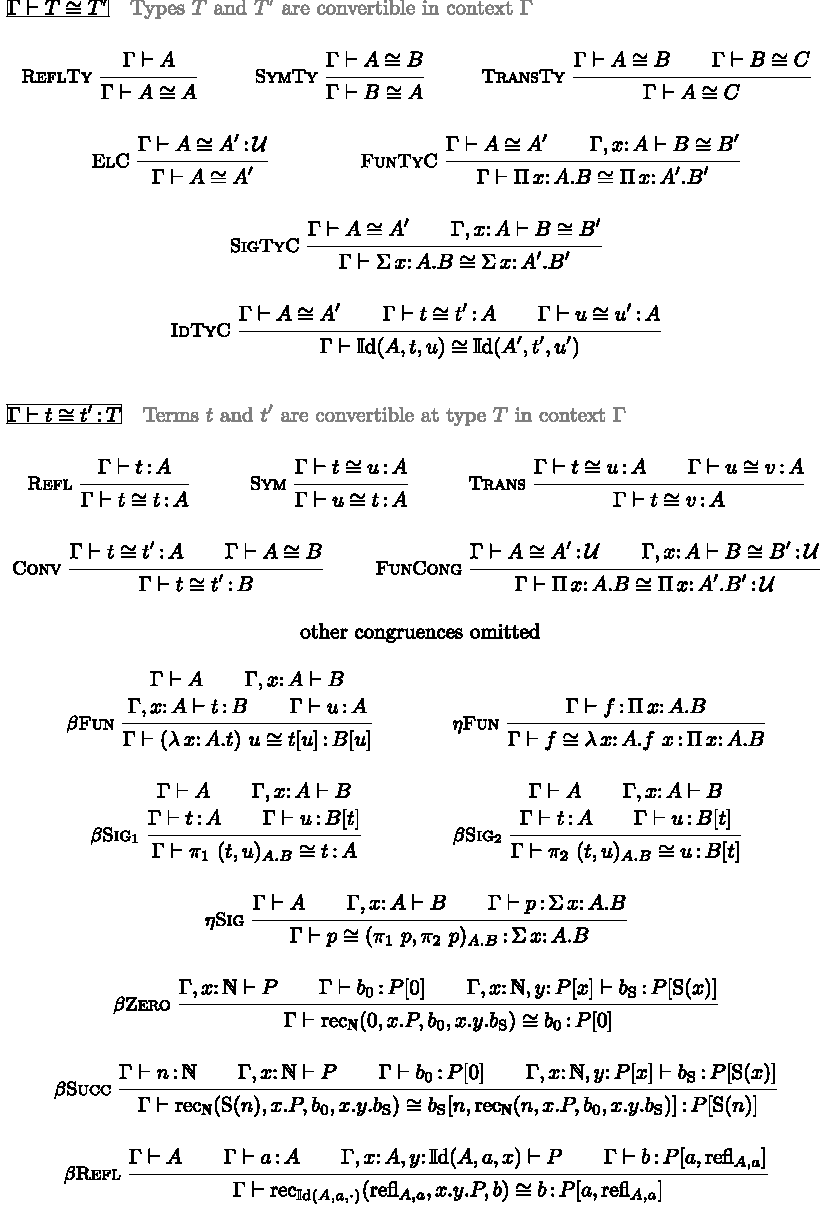
\includegraphics[width=0.98\linewidth,height=0.72\textheight,keepaspectratio]{rules-05.pdf}\end{center}
 
% END A1.SS1.p1
 
% END A1.SS1
 
% BEGIN A1.SS2
 
\par\medskip\noindent\textbf{A.2 Neutral comparison}\par
 
% BEGIN A1.SS2.p1
 
\begin{center}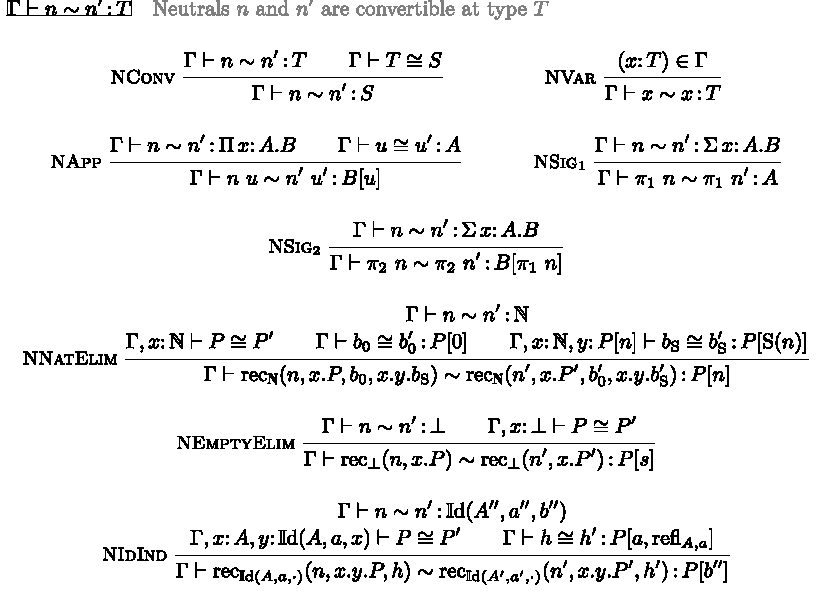
\includegraphics[width=0.98\linewidth,height=0.72\textheight,keepaspectratio]{rules-06.pdf}\end{center}
 
% END A1.SS2.p1
 
% END A1.SS2
 
% END A1


% BEGIN A2
 
\par\medskip\noindent\textbf{Appendix B Algorithmic Martin-Löf Type Theory}\par
 
% BEGIN A2.SS1
 
\par\medskip\noindent\textbf{B.1 Typed algorithmic conversion}\par
 
% BEGIN A2.SS1.p1
 
\begin{center}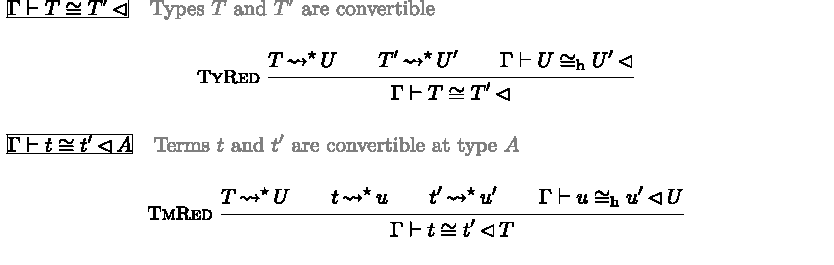
\includegraphics[width=0.98\linewidth,height=0.72\textheight,keepaspectratio]{rules-07.pdf}\end{center}
 
% END A2.SS1.p1
 
% BEGIN A2.SS1.p2
 
\begin{center}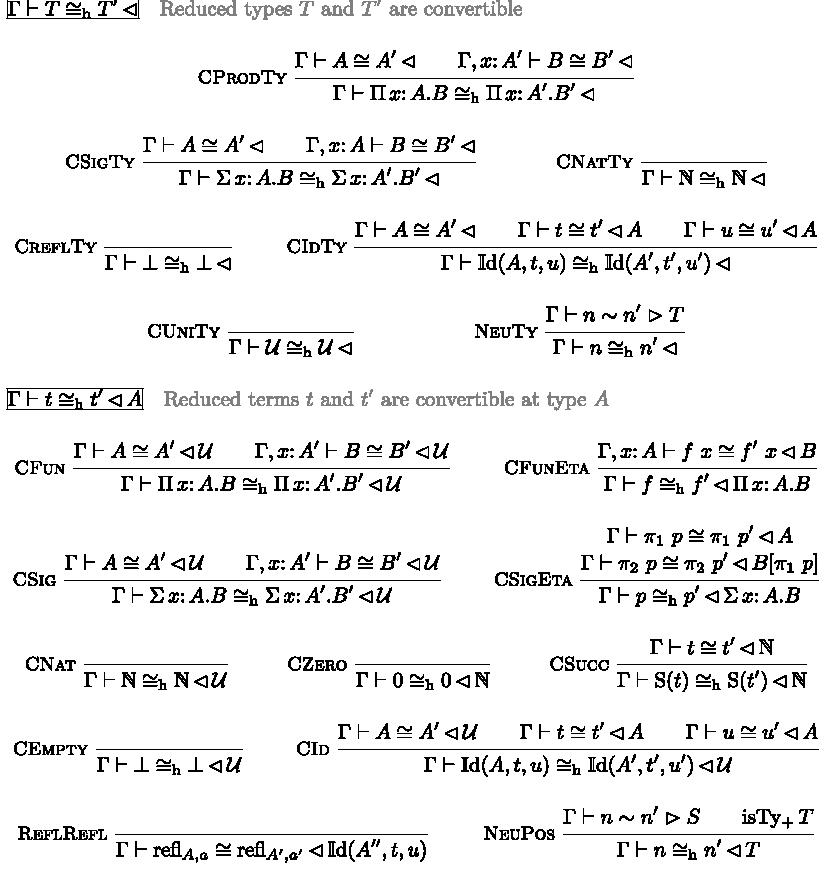
\includegraphics[width=0.98\linewidth,height=0.72\textheight,keepaspectratio]{rules-08.pdf}\end{center}
 
% END A2.SS1.p2
 
% BEGIN A2.SS1.p3
 
\begin{center}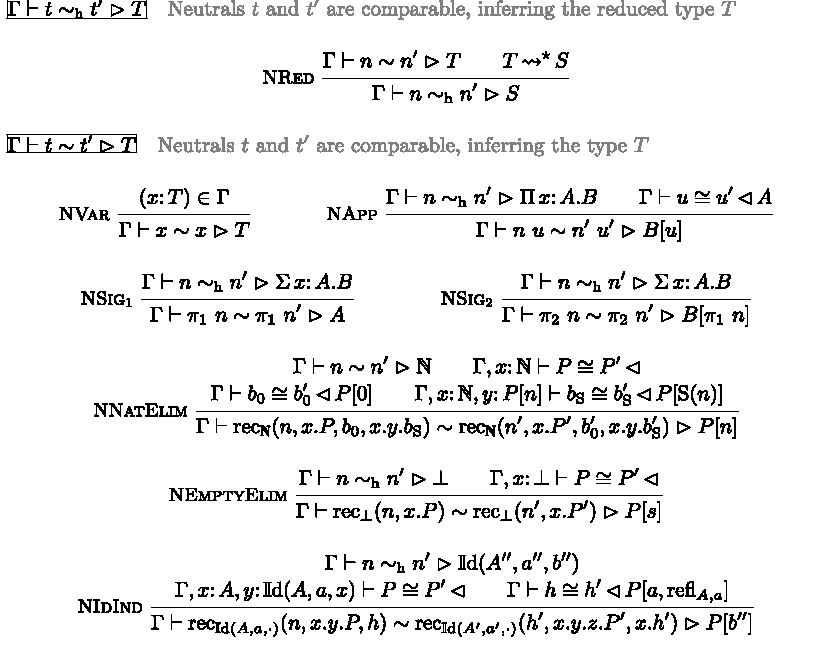
\includegraphics[width=0.98\linewidth,height=0.72\textheight,keepaspectratio]{rules-09.pdf}\end{center}
 
% END A2.SS1.p3
 
% END A2.SS1
 
% BEGIN A2.SS2
 
\par\medskip\noindent\textbf{B.2 Untyped algorithmic conversion}\par
 
% BEGIN A2.SS2.p1
 
\begin{center}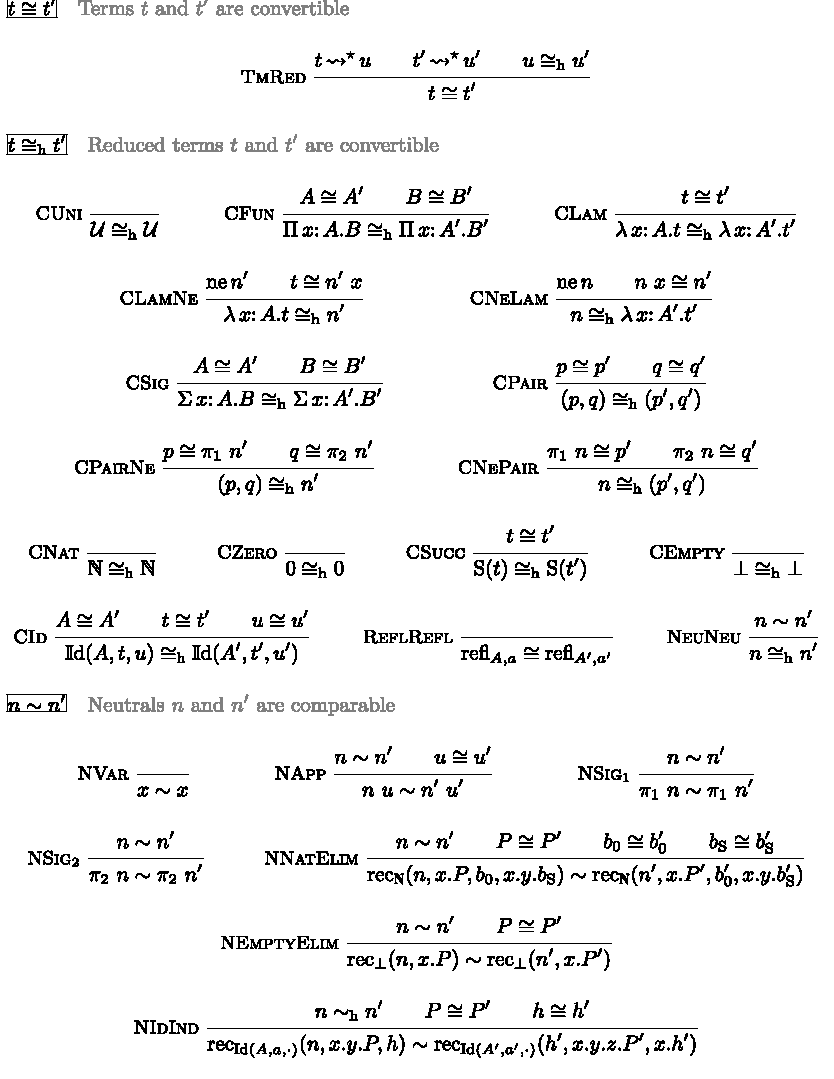
\includegraphics[width=0.98\linewidth,height=0.72\textheight,keepaspectratio]{rules-10.pdf}\end{center}
 
% END A2.SS2.p1
 
% BEGIN A2.SS2.p2
 
\par
 
% END A2.SS2.p2
 
% END A2.SS2
 
% END A2

% BEGIN Thmtheorem22
 
\par\medskip\noindent\textbf{Proposition 22 (  Typed to untyped conversion).}\par
 
% BEGIN Thmtheorem22.p1
 
Assuming Property 1, the typed algorithmic judgments imply their untyped counterparts whenever their preconditions hold.\par
 
% END Thmtheorem22.p1
 
% END Thmtheorem22

% BEGIN Thmtheorem24
 
\par\medskip\noindent\textbf{Proposition 24 (  Untyped to typed conversion).}\par
 
% BEGIN Thmtheorem24.p1
 
Assuming injectivity of typed constructors and deep normalisation, the untyped algorithmic judgments imply their typed counterparts whenever their preconditions hold.\par
 
% END Thmtheorem24.p1
 
% END Thmtheorem24

% BEGIN S4.SS3.SSS0.P0.SPx1
 
\par\medskip\noindent\textbf{Proof.}\par
 
% BEGIN S4.SS3.SSS0.P0.SPx1.p1
 
The proof is by bundled induction on the typed algorithmic judgment. We simultaneously prove that if $\Gamma\vdash n\mathrel{\raisebox{-0.5pt}{$\cong$}}n^{\prime}\operatorname{%
\mathrel{\lhd}}T$ and moreover $n$, $n^{\prime}$ are neutrals, then $n\sim n^{\prime}$.\par
 
% END S4.SS3.SSS0.P0.SPx1.p1
 
% BEGIN S4.SS3.SSS0.P0.SPx1.p2
 
The main interesting case is of course that of   Typed conversion algorithm (excerpt, see Sec.˜B.1).. In this case, the typing invariants imply, by Corollary 3, that both sides are either abstractions or neutrals. In the first three cases, we can directly conclude by induction hypothesis, up to $\beta$-reduction of the $\eta$-expanded abstraction. Remains the case of two neutrals $n$ and $n^{\prime}$. The extra induction hypothesis for neutrals tells us that $n\ y\sim n^{\prime}\ y$, or more precisely in de Bruijn syntax, that $n\mathord{\left[\uparrow\right]}\ y\sim n^{\prime}\mathord{\left[\uparrow%
\right]}\ y$, where $\uparrow$ is the substitution shifting all indices by 1. We can easily invert this to $n\mathord{\left[\uparrow\right]}\sim n^{\prime}\mathord{\left[\uparrow\right]}$, and conclude by an auxiliary lemma that untyped conversion admits strengthening. $\hfill\blacktriangleleft$ Note the final use of strengthening: while this is readily proven by induction for algorithmic judgments, it is generally difficult to prove for declarative systems! Admitting easy proofs of strengthening is a major advantage of algorithmic presentations [30].\par
 
% END S4.SS3.SSS0.P0.SPx1.p2
 
% BEGIN S4.SS3.SSS0.P0.SPx1.p3
 
For the converse, there is a catch: normalisation is required. Indeed, imagine a type $A$, well-formed in $\Gamma$, such that there is an infinite reduction sequence $A\operatorname{\rightsquigarrow}A_{1}\operatorname{\rightsquigarrow}\dots$ Trying to deduce $\Gamma,x:A\vdash x\mathrel{\raisebox{-0.5pt}{$\cong$}}x\operatorname{\mathrel{%
:}}A$, the untyped algorithm would terminate immediately, while the typed one would diverge on the evaluation of $A$. More insidiously, if a type $B$ keeps on exposing $\operatorname{\Pi}$ constructors – say a solution to $B\mathrel{\raisebox{-0.5pt}{$\cong$}}\operatorname{\mathbb{N}}\to B$ – comparing $x:B$ to itself would terminate immediately on one side, and spin in never ending $\eta$-expansions on the other. We can, however, prove the following crucial lemma.\par
 
% END S4.SS3.SSS0.P0.SPx1.p3
 
% BEGIN Thmtheorem23
 
\par\medskip\noindent\textbf{Lemma 23 (  Completeness of typed neutral conversion at all types).}\par
 
% BEGIN Thmtheorem23.p1
 
Assuming Property 11, given a context $\Gamma$ and $A$, $m$, $n$ respectively a well-formed type and well-typed terms in $\Gamma$, such that $\Gamma\vdash m\sim n\mathrel{\rhd}A^{\prime}$ and $\Gamma\vdash A^{\prime}\mathrel{\raisebox{-0.5pt}{$\cong$}}A$, we have $\Gamma\vdash m\mathrel{\raisebox{-0.5pt}{$\cong$}}n\operatorname{\mathrel{\lhd%
}}{A}$.\par
 
% END Thmtheorem23.p1
 
% END Thmtheorem23
 
% END S4.SS3.SSS0.P0.SPx1
 
% BEGIN S4.SS3.SSS0.P0.SPx2
 
\par\medskip\noindent\textbf{Proof sketch555In the formalisation, we shortcut this proof using the equivalence of declarative and algorithmic typing..}\par
 
% BEGIN S4.SS3.SSS0.P0.SPx2.p1
 
By induction on the deep normalisation of $A$, using which, after a series of $\eta$-expansions of $m$ and $n$, we end up at a positive type. At this point we go into neutral mode, peel off all introduced $\eta$-expansions, and use our neutral comparison hypothesis, adequately weakened to account for the extra introduced variables, to conclude. $\hfill\blacktriangleleft$\par
 
% END S4.SS3.SSS0.P0.SPx2.p1

% BEGIN S4.SS3.SSS0.P0.SPx2.p2
 
After Lemma 23, remains a straightforward induction – as usual, using preservation lemmas as necessary. However, let us emphasise that while the proof of equivalence is relatively direct, it nonetheless relies on difficult properties: strengthening, and normalisation.\par
 
% END S4.SS3.SSS0.P0.SPx2.p2
 
% END S4.SS3.SSS0.P0.SPx2
 
% END S4.SS3

\clearpage
\section*{Author formal definitions and typed/untyped equivalence proof}
Complete unchanged source files below are from the paper-linked repository snapshot 9ca549d553bd41a6c00efb0655d23fa9a8dabd48, under its original MIT license. The complete source project (including all imports and auxiliary proofs) is also attached as author-formal-snapshot.zip. No new proof-assistant execution is claimed.

\subsection*{theories/DeclarativeTyping.v}
\begin{lstlisting}
(** * LogRel.DeclarativeTyping: specification of conversion and typing, in a declarative fashion. *)
From Coq Require Import ssreflect.
From smpl Require Import Smpl.
From LogRel Require Import Utils Syntax.All.

Set Primitive Projections.

(** Definitions in this file should be understood as the _specification_ of conversion
or typing, done in a declarative fashion. For instance, we _demand_ that conversion
be transitive by adding a corresponding rule. *)

(** ** Definitions *)
Section Definitions.

  (* We locally disable typing notations to be able to use them in the definition
  here before declaring the instance to which abstract notations are bound. *)
  Close Scope typing_scope.


  (** Typing and conversion are mutually defined inductive relations. To avoid having
  to bother with elimination of propositions, we put them in the Type sort. *)

  (** **** Context well-formation *)
  Inductive WfContextDecl : context -> Type :=
      | connil : [ |- ε ]
      | concons {Γ A} : 
          [ |- Γ ] -> 
          [ Γ |- A ] -> 
          [ |-  Γ ,, A]
  (** **** Type well-formation *)
  with WfTypeDecl  : context -> term -> Type :=
      | wfTypeU {Γ} : 
          [ |- Γ ] -> 
          [ Γ |- U ] 
      | wfTypeProd {Γ} {A B} : 
          [ Γ |- A ] -> 
          [Γ ,, A |- B ] -> 
          [ Γ |- tProd A B ]
      | wfTypeNat {Γ} : 
          [|- Γ] ->
          [Γ |- tNat]
      | wfTypeEmpty {Γ} : 
          [|- Γ] ->
          [Γ |- tEmpty]
      | wfTypeSig {Γ} {A B} : 
          [ Γ |- A ] -> 
          [Γ ,, A |- B ] -> 
          [ Γ |- tSig A B ]
      | wftTypeId {Γ} {A x y} :
          [Γ |- A] ->
          [Γ |- x : A] ->
          [Γ |- y : A] ->
          [Γ |- tId A x y]
      | wfTypeUniv {Γ} {A} :
          [ Γ |- A : U ] -> 
          [ Γ |- A ]
  (** **** Typing *)
  with TypingDecl : context -> term -> term -> Type :=
      | wfVar {Γ} {n decl} :
          [   |- Γ ] ->
          in_ctx Γ n decl ->
          [ Γ |- tRel n : decl ]
      | wfTermProd {Γ} {A B} :
          [ Γ |- A : U] -> 
          [Γ ,, A |- B : U ] ->
          [ Γ |- tProd A B : U ]
      | wfTermLam {Γ} {A B t} :
          [ Γ |- A ] ->        
          [ Γ ,, A |- t : B ] -> 
          [ Γ |- tLambda A t : tProd A B]
      | wfTermApp {Γ} {f a A B} :
          [ Γ |- f : tProd A B ] -> 
          [ Γ |- a : A ] -> 
          [ Γ |- tApp f a : B[a..] ]
      | wfTermNat {Γ} :
          [|-Γ] ->
          [Γ |- tNat : U]
      | wfTermZero {Γ} :
          [|-Γ] ->
          [Γ |- tZero : tNat]
      | wfTermSucc {Γ n} :
          [Γ |- n : tNat] ->
          [Γ |- tSucc n : tNat]
      | wfTermNatElim {Γ P hz hs n} :
        [Γ ,, tNat |- P ] ->
        [Γ |- hz : P[tZero..]] ->
        [Γ |- hs : elimSuccHypTy P] ->
        [Γ |- n : tNat] ->
        [Γ |- tNatElim P hz hs n : P[n..]]
      | wfTermEmpty {Γ} :
          [|-Γ] ->
          [Γ |- tEmpty : U]
      | wfTermEmptyElim {Γ P e} :
        [Γ ,, tEmpty |- P ] ->
        [Γ |- e : tEmpty] ->
        [Γ |- tEmptyElim P e : P[e..]]
      | wfTermSig {Γ} {A B} :
        [ Γ |- A : U] -> 
        [Γ ,, A |- B : U ] ->
        [ Γ |- tSig A B : U ]
      | wfTermPair {Γ} {A B a b} :
        [Γ |- A] ->
        [Γ,, A |- B] ->
        [Γ |- a : A] -> 
        [Γ |- b : B[a..]] ->
        [Γ |- tPair A B a b : tSig A B]
      | wfTermFst {Γ A B p} :
        [Γ |- p : tSig A B] ->
        [Γ |- tFst p : A]
      | wfTermSnd {Γ A B p} :
        [Γ |- p : tSig A B] ->
        [Γ |- tSnd p : B[(tFst p)..]]
      | wfTermId {Γ} {A x y} :
          [Γ |- A : U] ->
          [Γ |- x : A] ->
          [Γ |- y : A] ->
          [Γ |- tId A x y : U]
      | wfTermRefl {Γ A x} :
          [Γ |- A] ->
          [Γ |- x : A] ->
          [Γ |- tRefl A x : tId A x x]
      | wfTermIdElim {Γ A x P hr y e} :
          [Γ |- A] ->
          [Γ |- x : A] ->
          [Γ ,, A ,, tId A⟨@wk1 Γ A⟩ x⟨@wk1 Γ A⟩ (tRel 0) |- P] ->
          [Γ |- hr : P[tRefl A x .: x..]] ->
          [Γ |- y : A] ->
          [Γ |- e : tId A x y] ->
          [Γ |- tIdElim A x P hr y e : P[e .: y..]]
      | wfTermConv {Γ} {t A B} :
          [ Γ |- t : A ] -> 
          [ Γ |- A ≅ B ] -> 
          [ Γ |- t : B ]
  (** **** Conversion of types *)
  with ConvTypeDecl : context -> term -> term  -> Type :=  
      | TypePiCong {Γ} {A B C D} :
          [ Γ |- A] ->
          [ Γ |- A ≅ B] ->
          [ Γ ,, A |- C ≅ D] ->
          [ Γ |- tProd A C ≅ tProd B D]
      | TypeSigCong {Γ} {A B C D} :
          [ Γ |- A] ->
          [ Γ |- A ≅ B] ->
          [ Γ ,, A |- C ≅ D] ->
          [ Γ |- tSig A C ≅ tSig B D]
      | TypeIdCong {Γ A A' x x' y y'} :
          (* [Γ |- A] -> ?  *)
          [Γ |- A ≅ A'] ->
          [Γ |- x ≅ x' : A] ->
          [Γ |- y ≅ y' : A] ->
          [Γ |- tId A x y ≅ tId A' x' y' ]
      | TypeRefl {Γ} {A} : 
          [ Γ |- A ] ->
          [ Γ |- A ≅ A]
      | convUniv {Γ} {A B} :
        [ Γ |- A ≅ B : U ] -> 
        [ Γ |- A ≅ B ]
      | TypeSym {Γ} {A B} :
          [ Γ |- A ≅ B ] ->
          [ Γ |- B ≅ A ]
      | TypeTrans {Γ} {A B C} :
          [ Γ |- A ≅ B] ->
          [ Γ |- B ≅ C] ->
          [ Γ |- A ≅ C]
  (** **** Conversion of terms *)
  with ConvTermDecl : context -> term -> term -> term -> Type :=
      | TermBRed {Γ} {a t A B} :
              [ Γ |- A ] ->
              [ Γ ,, A |- t : B ] ->
              [ Γ |- a : A ] ->
              [ Γ |- tApp (tLambda A t) a ≅ t[a..] : B[a..] ]
      | TermPiCong {Γ} {A B C D} :
          [ Γ |- A : U] ->
          [ Γ |- A ≅ B : U ] ->
          [ Γ ,, A |- C ≅ D : U ] ->
          [ Γ |- tProd A C ≅ tProd B D : U ]
      | TermAppCong {Γ} {a b f g A B} :
          [ Γ |- f ≅ g : tProd A B ] ->
          [ Γ |- a ≅ b : A ] ->
          [ Γ |- tApp f a ≅ tApp g b : B[a..] ]
      | TermLambdaCong {Γ} {t u A A' A'' B} :
          [ Γ |- A ] ->
          [ Γ |- A ≅ A' ] ->
          [ Γ |- A ≅ A'' ] ->
          [ Γ,, A |- t ≅ u : B ] ->
          [ Γ |- tLambda A' t ≅ tLambda A'' u : tProd A B ]
      | TermFunEta {Γ} {f A B} :
          [ Γ |- f : tProd A B ] ->
          [ Γ |- tLambda A (eta_expand f) ≅ f : tProd A B ]
      | TermSuccCong {Γ} {n n'} :
          [Γ |- n ≅ n' : tNat] ->
          [Γ |- tSucc n ≅ tSucc n' : tNat]
      | TermNatElimCong {Γ P P' hz hz' hs hs' n n'} :
          [Γ ,, tNat |- P ≅ P'] ->
          [Γ |- hz ≅ hz' : P[tZero..]] ->
          [Γ |- hs ≅ hs' : elimSuccHypTy P] ->
          [Γ |- n ≅ n' : tNat] ->
          [Γ |- tNatElim P hz hs n ≅ tNatElim P' hz' hs' n' : P[n..]]        
      | TermNatElimZero {Γ P hz hs} :
          [Γ ,, tNat |- P ] ->
          [Γ |- hz : P[tZero..]] ->
          [Γ |- hs : elimSuccHypTy P] ->
          [Γ |- tNatElim P hz hs tZero ≅ hz : P[tZero..]]
      | TermNatElimSucc {Γ P hz hs n} :
          [Γ ,, tNat |- P ] ->
          [Γ |- hz : P[tZero..]] ->
          [Γ |- hs : elimSuccHypTy P] ->
          [Γ |- n : tNat] ->
          [Γ |- tNatElim P hz hs (tSucc n) ≅ tApp (tApp hs n) (tNatElim P hz hs n) : P[(tSucc n)..]]
      | TermEmptyElimCong {Γ P P' e e'} :
          [Γ ,, tEmpty |- P ≅ P'] ->
          [Γ |- e ≅ e' : tEmpty] ->
          [Γ |- tEmptyElim P e ≅ tEmptyElim P' e' : P[e..]]
      | TermSigCong {Γ} {A A' B B'} :
          [ Γ |- A : U] ->
          [ Γ |- A ≅ A' : U ] ->
          [ Γ ,, A |- B ≅ B' : U ] ->
          [ Γ |- tSig A B ≅ tSig A' B' : U ]
      | TermPairCong {Γ A A' A'' B B' B'' a a' b b'} :
          [Γ |- A] ->
          [Γ |- A ≅ A'] ->
          [Γ |- A ≅ A''] ->
          [Γ,, A |- B ≅ B'] ->
          [Γ,, A |- B ≅ B''] ->
          [Γ |- a ≅ a' : A] ->
          [Γ |- b ≅ b' : B[a..]] ->
          [Γ |- tPair A' B' a b ≅ tPair A'' B'' a' b' : tSig A B]
      | TermPairEta {Γ} {A B p} :
          [Γ |- p : tSig A B] ->
          [Γ |- tPair A B (tFst p) (tSnd p) ≅ p : tSig A B]
      | TermFstCong {Γ A B p p'} :
        [Γ |- p ≅ p' : tSig A B] ->
        [Γ |- tFst p ≅ tFst p' : A]
      | TermFstBeta {Γ A B a b} :
        [Γ |- A] ->
        [Γ ,, A |- B] ->
        [Γ |- a : A] ->
        [Γ |- b : B[a..]] ->
        [Γ |- tFst (tPair A B a b) ≅ a : A]
      | TermSndCong {Γ A B p p'} :
        [Γ |- p ≅ p' : tSig A B] ->
        [Γ |- tSnd p ≅ tSnd p' : B[(tFst p)..]]
      | TermSndBeta {Γ A B a b} :
        [Γ |- A] ->
        [Γ ,, A |- B] ->
        [Γ |- a : A] ->
        [Γ |- b : B[a..]] ->
        [Γ |- tSnd (tPair A B a b) ≅ b : B[(tFst (tPair A B a b))..]]
      | TermIdCong {Γ A A' x x' y y'} :
        (* [Γ |- A] -> ?  *)
        [Γ |- A ≅ A' : U] ->
        [Γ |- x ≅ x' : A] ->
        [Γ |- y ≅ y' : A] ->
        [Γ |- tId A x y ≅ tId A' x' y' : U ]
      | TermReflCong {Γ A A' x x'} :
        [Γ |- A ≅ A'] ->
        [Γ |- x ≅ x' : A] ->
        [Γ |- tRefl A x ≅ tRefl A' x' : tId A x x]
      | TermIdElim {Γ A A' x x' P P' hr hr' y y' e e'} :
        (* Parameters well formed: required for stability by weakening,
          in order to show that the context Γ ,, A ,, tId A⟨@wk1 Γ A⟩ x⟨@wk1 Γ A⟩ (tRel 0)
          remains well-formed under weakenings *)
        [Γ |- A] ->
        [Γ |- x : A] ->
        [Γ |- A ≅ A'] ->
        [Γ |- x ≅ x' : A] ->
        [Γ ,, A ,, tId A⟨@wk1 Γ A⟩ x⟨@wk1 Γ A⟩ (tRel 0) |- P ≅ P'] ->
        [Γ |- hr ≅ hr' : P[tRefl A x .: x..]] ->
        [Γ |- y ≅ y' : A] ->
        [Γ |- e ≅ e' : tId A x y] ->
        [Γ |- tIdElim A x P hr y e ≅ tIdElim A' x' P' hr' y' e' : P[e .: y..]]
      | TermIdElimRefl {Γ A x P hr y A' z} :
        [Γ |- A] ->
        [Γ |- x : A] ->
        [Γ ,, A ,, tId A⟨@wk1 Γ A⟩ x⟨@wk1 Γ A⟩ (tRel 0) |- P] ->
        [Γ |- hr : P[tRefl A x .: x..]] ->
        [Γ |- y : A] ->
        [Γ |- A'] ->
        [Γ |- z : A] ->
        [Γ |- A ≅ A'] ->
        [Γ |- x ≅ y : A] ->
        [Γ |- x ≅ z : A] ->
        [Γ |- tIdElim A x P hr y (tRefl A' z) ≅ hr : P[tRefl A' z .: y..]]
      | TermRefl {Γ} {t A} :
          [ Γ |- t : A ] -> 
          [ Γ |- t ≅ t : A ]
      | TermConv {Γ} {t t' A B} :
          [ Γ |- t ≅ t': A ] ->
          [ Γ |- A ≅ B ] ->
          [ Γ |- t ≅ t': B ]
      | TermSym {Γ} {t t' A} :
          [ Γ |- t ≅ t' : A ] ->
          [ Γ |- t' ≅ t : A ]
      | TermTrans {Γ} {t t' t'' A} :
          [ Γ |- t ≅ t' : A ] ->
          [ Γ |- t' ≅ t'' : A ] ->
          [ Γ |- t ≅ t'' : A ]
      
  where "[   |- Γ ]" := (WfContextDecl Γ)
  and   "[ Γ |- T ]" := (WfTypeDecl Γ T)
  and   "[ Γ |- t : T ]" := (TypingDecl Γ T t)
  and   "[ Γ |- A ≅ B ]" := (ConvTypeDecl Γ A B)
  and   "[ Γ |- t ≅ t' : T ]" := (ConvTermDecl Γ T t t').

  (** (Typed) reduction is defined afterwards,
  rather than mutually with the other relations. *)

  Local Coercion isterm : term >-> class.

  Record RedClosureDecl (Γ : context) (A : class) (t u : term) := {
    reddecl_typ : match A with istype => [Γ |- t] | isterm A => [Γ |- t : A] end;
    reddecl_red : RedClosureAlg t u;
    reddecl_conv : match A with istype => [ Γ |- t ≅ u ] | isterm A => [Γ |- t ≅ u : A] end;
  }.

  Notation "[ Γ |- t (*@{\proofwavefont ⤳}@*)* t' ∈ A ]" := (RedClosureDecl Γ A t t').

(** ** Declarative neutral conversion *)

(** We have two notions of "convertible neutrals". The first is relatively weak, and says only that
  the two terms are neutral and are convertible (wrt. standard conversion). The good side is that
  it can be shown to satisfy the interface of generic typing already. The bad side is that it does not
  give us strong enough inversion principles. *)

  Record WeakDeclNeutralConversion (Γ : context) (A : term) (t u : term) := {
    convnedecl_whne_l : whne t;
    convnedecl_whne_r : whne u;
    convnedecl_conv : [ Γ |- t ≅ u : A ];
  }.

(** The second, much stronger notion compares neutrals only "structurally".
  In particular, it does *not* embed transitivity.
  The price is that at this stage we cannot show that it is transitive, yet – we need injectivity of
  type constructors for that. So we defer that until that later point. *)

  Inductive DeclNeutralConversion (Γ : context) : term -> term -> term -> Type :=

  | neuConvRel T n : [|- Γ] -> in_ctx Γ n T -> [Γ |- tRel n ~ tRel n : T]

  | neuConvApp A B n n' a a' :
      [Γ |- n ~ n' : tProd A B] ->
      [Γ |- a ≅ a' : A] ->
      [Γ |- tApp n a ~ tApp n' a' : B[a..]]

  | neuConvNat {P P' hz hz' hs hs' n n'} :
      [Γ |- n ~ n' : tNat] ->
      [Γ ,, tNat |- P ≅ P'] ->
      [Γ |- hz ≅ hz' : P[tZero..]] ->
      [Γ |- hs ≅ hs' : elimSuccHypTy P] ->
      [Γ |- tNatElim P hz hs n ~ tNatElim P' hz' hs' n' : P[n..]]

  | neuConvEmpty {P P' e e'} :
      [Γ ,, tEmpty |- P ≅ P'] ->
      [Γ |- e ~ e' : tEmpty] ->
      [Γ |- tEmptyElim P e ~ tEmptyElim P' e' : P[e..]]

  | neuConvFst {A B p p'} :
      [Γ |- p ~ p' : tSig A B] ->
      [Γ |- tFst p ~ tFst p' : A]

  | neuConvSnd {A B p p'} :
      [Γ |- p ~ p' : tSig A B] ->
      [Γ |- tSnd p ~ tSnd p' : B[(tFst p)..]]

  | neuConvId {A A' x x' P P' hr hr' y y' e e'} :
      [Γ |- A ≅ A'] ->
      [Γ |- x ≅ x' : A] ->
      [Γ ,, A ,, tId A⟨@wk1 Γ A⟩ x⟨@wk1 Γ A⟩ (tRel 0) |- P ≅ P'] ->
      [Γ |- hr ≅ hr' : P[tRefl A x .: x..]] ->
      [Γ |- y ≅ y' : A] ->
      [Γ |- e ~ e' : tId A x y] ->
      [Γ |- tIdElim A x P hr y e ~ tIdElim A' x' P' hr' y' e' : P[e .: y..]]

  | neuConvConv {A B n n'} :
      [Γ |- n ~ n' : A] ->
      [Γ |- A ≅ B] ->
      [Γ |- n ~ n' : B]

  where "[ Γ |- m ~ n : A ]" := (DeclNeutralConversion Γ A m n).

End Definitions.

Definition TermRedClosure Γ A t u := RedClosureDecl Γ (isterm A) t u.
Definition TypeRedClosure Γ A B := RedClosureDecl Γ istype A B.

Notation "[ Γ |- t (*@{\proofwavefont ⤳}@*)* u ∈ A ]" := (RedClosureDecl Γ A t u).

(** ** Instances *)
(** Used for printing (see Notations) and as a support for the generic typing
properties used for the logical relation (see GenericTyping). *)
Module DeclarativeTypingData.

  Definition de : tag.
  Proof.
  constructor.
  Qed.

  #[export] Instance WfContext_Decl : WfContext de := WfContextDecl.
  #[export] Instance WfType_Decl : WfType de := WfTypeDecl.
  #[export] Instance Typing_Decl : Typing de := TypingDecl.
  #[export] Instance ConvType_Decl : ConvType de := ConvTypeDecl.
  #[export] Instance ConvTerm_Decl : ConvTerm de := ConvTermDecl.
  #[export] Instance RedType_Decl : RedType de := TypeRedClosure.
  #[export] Instance RedTerm_Decl : RedTerm de := TermRedClosure.
  #[export] Instance ConvNeuConv_Decl : ConvNeuConv de := DeclNeutralConversion.

  Ltac fold_decl :=
    change WfContextDecl with (wf_context (ta := de)) in * ;
    change WfTypeDecl with (wf_type (ta := de)) in *;
    change TypingDecl with (typing (ta := de)) in * ;
    change ConvTypeDecl with (conv_type (ta := de)) in * ;
    change ConvTermDecl with (conv_term (ta := de)) in * ;
    change TypeRedClosure with (red_ty (ta := de)) in *;
    change TermRedClosure with (red_tm (ta := de)) in *;
    change DeclNeutralConversion with (conv_neu_ty (ta := de)) in *.

  Smpl Add fold_decl : refold.

End DeclarativeTypingData.

(** This weaker instance is necessary to break circularity: indeed, we can only derive
  that the above instance is an instance of generic typing once we have injectivity
  of type constructors, because we need said injectivity to show that neutral conversion
  is transitive. So we will first instantiate the logical relation once with this
  weaker instance, obtain injectivity of type constructors, then derive that the above
  instance is also an instance of generic typing, then instantiate the logical relation again.
*)
Module WeakDeclarativeTypingData.

  Import DeclarativeTypingData.
  #[export] Remove Hints DeclNeutralConversion : typeclass_instances.
  #[export] Instance ConvNeuConv_WeakDecl : ConvNeuConv de := WeakDeclNeutralConversion.

End WeakDeclarativeTypingData.

Import DeclarativeTypingData.

(** ** Induction principles *)

(** We use Scheme to generate mutual induction principle. Sadly, Scheme uses
the product of the standard library, which is not universe polymorphic, which
causes universe issues, typically in the fundamental lemma. So
we use some Ltac code to generate properly polymorphic versions of the inductive
principle. We also use Ltac to generate the conclusion of the mutual induction
proof, to alleviate the user from the need to write it down every time: they
only need write the predicates to be proven. *)
Section InductionPrinciples.

Scheme 
    Minimality for WfContextDecl Sort Type with
    Minimality for WfTypeDecl   Sort Type with
    Minimality for TypingDecl    Sort Type with
    Minimality for ConvTypeDecl  Sort Type with
    Minimality for ConvTermDecl  Sort Type.

Combined Scheme _WfDeclInduction from
    WfContextDecl_rect_nodep,
    WfTypeDecl_rect_nodep,
    TypingDecl_rect_nodep,
    ConvTypeDecl_rect_nodep,
    ConvTermDecl_rect_nodep.

Let _WfDeclInductionType :=
  ltac:(let ind := fresh "ind" in
      pose (ind := _WfDeclInduction);
      refold ;
      let ind_ty := type of ind in
      exact ind_ty).

Let WfDeclInductionType :=
  ltac: (let ind := eval cbv delta [_WfDeclInductionType] zeta
    in _WfDeclInductionType in
    let ind' := polymorphise ind in
  exact ind').

Lemma WfDeclInduction : WfDeclInductionType.
Proof.
  intros PCon PTy PTm PTyEq PTmEq **.
  pose proof (_WfDeclInduction PCon PTy PTm PTyEq PTmEq) as H.
  destruct H as [?[?[? []]]].
  all: try (assumption ; fail).
  repeat (split;[assumption|]); assumption.
Qed.

Definition WfDeclInductionConcl :=
  ltac:(
    let t := eval cbv delta [WfDeclInductionType] beta in WfDeclInductionType in
    let t' := remove_steps t in
    exact t').

End InductionPrinciples.

Arguments WfDeclInductionConcl PCon PTy PTm PTyEq PTmEq : rename.

(** ** Generation *)

(** The generation lemma (the name comes from the PTS literature), gives a 
stronger inversion principle on typing derivations, that give direct access
to the last non-conversion rule, and bundle together all conversions.

Note that because we do not yet know that [Γ |- t : T] implies [Γ |- T],
we cannot use reflexivity in the case where the last rule was not a conversion
one, and we get the slightly clumsy disjunction of either an equality or a
conversion proof. We get a better version of generation later on, once we have
this implication. *)

Definition termGenData (Γ : context) (t T : term) : Type :=
  match t with
    | tRel n => ∑ decl, [× T = decl, [|- Γ]& in_ctx Γ n decl]
    | tProd A B =>  [× T = U, [Γ |- A : U] & [Γ,, A |- B : U]]
    | tLambda A t => ∑ B, [× T = tProd A B, [Γ |- A] & [Γ,, A |- t : B]]
    | tApp f a => ∑ A B, [× T = B[a..], [Γ |- f : tProd A B] & [Γ |- a : A]]
    | tSort _ => False
    | tNat => T = U
    | tZero => T = tNat
    | tSucc n => T = tNat × [Γ |- n : tNat]
    |  tNatElim P hz hs n =>
      [× T = P[n..], [Γ,, tNat |- P], [Γ |- hz : P[tZero..]], [Γ |- hs : elimSuccHypTy P] & [Γ |- n : tNat]]
    | tEmpty => T = U
    | tEmptyElim P e =>
      [× T = P[e..], [Γ,, tEmpty |- P] & [Γ |- e : tEmpty]]
    | tSig A B => [× T = U, [Γ |- A : U] & [Γ ,, A |- B : U]]
    | tPair A B a b =>
     [× T = tSig A B, [Γ |- A], [Γ,, A |- B], [Γ |- a : A] & [Γ |- b : B[a..]]]
    | tFst p => ∑ A B, T = A × [Γ |- p : tSig A B]
    | tSnd p => ∑ A B, T = B[(tFst p)..] × [Γ |- p : tSig A B]
    | tId A x y => [× T = U, [Γ |- A : U], [Γ |- x : A] & [Γ |- y : A]]
    | tRefl A x => [× T = tId A x x, [Γ |- A] & [Γ |- x : A]]
    | tIdElim A x P hr y e => 
      [× T = P[e .: y..], [Γ |- A], [Γ |- x : A], [Γ,, A,, tId A⟨@wk1 Γ A⟩ x⟨@wk1 Γ A⟩ (tRel 0) |- P], [Γ |- hr : P[tRefl A x .: x..]], [Γ |- y : A] & [Γ |- e : tId A x y]]
  end.

(* Use `termGen` from later on instead after this file. *)
Lemma _termGen Γ t A :
  [Γ |- t : A] ->
  ∑ A', (termGenData Γ t A') × ((A' = A) + [Γ |- A' ≅ A]).
Proof.
  induction 1.
  all: try (eexists ; split ; [..|left ; reflexivity] ; cbn ; by_prod_splitter).
  + destruct IHTypingDecl as [? [? [-> | ]]].
    * prod_splitter; tea; now right.
    * prod_splitter; tea; right; now eapply TypeTrans.
Qed.

Lemma prod_ty_inv Γ A B :
  [Γ |- tProd A B] ->
  [Γ |- A] × [Γ,, A |- B].
Proof.
  intros Hty.
  inversion Hty ; subst ; refold.
  - easy.
  - eapply _termGen in H as (?&[]&_) ; subst.
    split ; now econstructor.
Qed.

Lemma sig_ty_inv Γ A B :
  [Γ |- tSig A B] ->
  [Γ |- A] × [Γ,, A |- B].
Proof.
  intros Hty.
  inversion Hty ; subst ; refold.
  - easy.
  - eapply _termGen in H as (?&[]&_) ; subst.
    split ; now econstructor.
Qed.

Lemma id_ty_inv Γ A x y :
  [Γ |- tId A x y] ->
  [× [Γ |- A], [Γ |- x : A] & [Γ |- y : A]].
Proof.
  intros Hty.
  inversion Hty ; subst ; refold.
  - easy.
  - eapply _termGen in H as (?&[]&_) ; subst.
    split ; try easy ; now econstructor.
Qed.

Lemma neutral_ty_inv Γ A :
  [Γ |- A] -> whne A -> [Γ |- A : U].
Proof.
  intros Hty Hne.
  inversion Hty ; subst ; refold.
  1-6: inversion Hne.
  easy.
Qed.
\end{lstlisting}

\subsection*{theories/AlgorithmicJudgments.v}
\begin{lstlisting}
(** * LogRel.AlgorithmicJudgments: definition of conversion (typed and untyped) and algorithmic typing, as inductive predicates. *)
From Coq Require Import ssrbool.
From LogRel Require Import Utils Syntax.All GenericTyping.

Section Definitions.

  (** We locally disable typing notations to be able to use them in the definition
  here before declaring the right instance. *)
  Close Scope typing_scope.

(** ** Typed conversion *)

  (** **** Conversion of types *)
  Inductive ConvTypeAlg : context -> term -> term  -> Type :=
    | typeConvRed {Γ A A' B B'} :
      [A (*@{\proofwavefont ⤳}@*)* A'] ->
      [B (*@{\proofwavefont ⤳}@*)* B'] ->
      [Γ |- A' ≅h B'] ->
      [Γ |- A ≅ B]
  (** **** Conversion of types reduced to weak-head normal forms *)
  with ConvTypeRedAlg : context -> term -> term -> Type :=
    | typePiCongAlg {Γ A B A' B'} :
      [ Γ |- A ≅ A'] ->
      [ Γ ,, A |- B ≅ B'] ->
      [ Γ |- tProd A B ≅h tProd A' B']
    | typeUnivConvAlg {Γ} :
      [Γ |- U ≅h U]
    | typeNatConvAlg {Γ} :
      [Γ |- tNat ≅h tNat]
    | typeEmptyConvAlg {Γ} :
      [Γ |- tEmpty ≅h tEmpty]
    | typeSigCongAlg {Γ A B A' B'} :
      [ Γ |- A ≅ A'] ->
      [ Γ ,, A |- B ≅ B'] ->
      [ Γ |- tSig A B ≅h tSig A' B']
    | typeIdCongAlg {Γ A A' x x' y y'} :
      [ Γ |- A ≅ A'] ->
      [ Γ |- x ≅ x' : A] ->
      [ Γ |- y ≅ y' : A] ->
      [ Γ |- tId A x y ≅h tId A' x' y']
    | typeNeuConvAlg {Γ M N T} :
      whne M ->
      whne N ->
      [ Γ |- M ~ N ▹ T] -> 
      [ Γ |- M ≅h N]
  (** **** Conversion of neutral terms *)
  with ConvNeuAlg : context -> term -> term  -> term -> Type :=
    | neuVarConvAlg {Γ n decl} :
      in_ctx Γ n decl ->
      [Γ |- tRel n ~ tRel n ▹ decl]
    | neuAppCongAlg {Γ m n t u A B} :
      [ Γ |- m ~h n ▹ tProd A B ] ->
      [ Γ |- t ≅ u : A ] ->
      [ Γ |- tApp m t ~ tApp n u ▹ B[t..] ]
    | neuNatElimCong {Γ n n' P P' hz hz' hs hs'} :
    (** Here, we know by invariant that the inferred type has to be tNat,
    so there should be no need to check that, but with parameterized/indexed
    inductive we need to recover informations from the neutrals to construct
    the context for the predicate and the type of the branches. *)
      [Γ |- n ~h n' ▹ tNat] ->
      [Γ,, tNat |- P ≅ P'] ->
      [Γ |- hz ≅ hz' : P[tZero..]] ->
      [Γ |- hs ≅ hs' : elimSuccHypTy P] ->
      [Γ |- tNatElim P hz hs n ~ tNatElim P' hz' hs' n' ▹ P[n..]]
    | neuEmptyElimCong {Γ P P' e e'} :
      [Γ |- e ~h e' ▹ tEmpty] ->
      [Γ ,, tEmpty |- P ≅ P'] ->
      [Γ |- tEmptyElim P e ~ tEmptyElim P' e' ▹ P[e..]]
    | neuFstCongAlg {Γ m n A B} :
      [ Γ |- m ~h n ▹ tSig A B ] ->
      [ Γ |- tFst m ~ tFst n ▹ A ]
    | neuSndCongAlg {Γ m n A B} :
      [ Γ |- m ~h n ▹ tSig A B ] ->
      [ Γ |- tSnd m ~ tSnd n ▹ B[(tFst m)..] ]
    | neuIdElimCong {Γ A A' A'' x x' x'' P P' hr hr' y y' y'' e e'} :
      [Γ |- e ~h e' ▹ tId A'' x'' y''] ->
      [Γ ,, A ,, tId A⟨@wk1 Γ A⟩ x⟨@wk1 Γ A⟩ (tRel 0) |- P ≅ P'] ->
      [Γ |- hr ≅ hr' : P[tRefl A x .: x..]] ->
      [Γ |- tIdElim A x P hr y e ~ tIdElim A' x' P' hr' y' e' ▹ P[e .: y..] ]
  (** **** Conversion of neutral terms at a type reduced to weak-head normal form*)
  with ConvNeuRedAlg : context -> term -> term -> term -> Type :=
    | neuConvRed {Γ m n A A'} :
      [Γ |- m ~ n ▹ A] ->
      [A (*@{\proofwavefont ⤳}@*)* A'] ->
      whnf A' ->
      [Γ |- m ~h n ▹ A']
  (** **** Conversion of terms *)
  with ConvTermAlg : context -> term -> term -> term -> Type :=
    | termConvRed {Γ t t' u u' A A'} :
      [A (*@{\proofwavefont ⤳}@*)* A'] ->
      [t (*@{\proofwavefont ⤳}@*)* t'] ->
      [u (*@{\proofwavefont ⤳}@*)* u' ] ->
      [Γ |- t' ≅h u' : A'] ->
      [Γ |- t ≅ u : A]
  (** **** Conversion of terms reduced to a weak-head normal form at a reduced type *)
  with ConvTermRedAlg : context -> term -> term -> term -> Type :=
    | termPiCongAlg {Γ A B A' B'} :
      [ Γ |- A ≅ A' : U] ->
      [ Γ ,, A |- B ≅ B' : U] ->
      [ Γ |- tProd A B ≅h tProd A' B' : U]
    | termNatReflAlg {Γ} :
      [Γ |- tNat ≅h tNat : U]
    | termZeroReflAlg {Γ} :
      [Γ |- tZero ≅h tZero : tNat]
    | termSuccCongAlg {Γ t t'} :
      [Γ |- t ≅ t' : tNat] ->
      [Γ |- tSucc t ≅h tSucc t' : tNat]
    | termEmptyReflAlg {Γ} :
      [Γ |- tEmpty ≅h tEmpty : U]
    | termFunConvAlg {Γ : context} {f g A B} :
      whnf f ->
      whnf g ->
      [ Γ,, A |- eta_expand f ≅ eta_expand g : B] -> 
      [ Γ |- f ≅h g : tProd A B]
    | termSigCongAlg {Γ A B A' B'} :
      [ Γ |- A ≅ A' : U] ->
      [ Γ ,, A |- B ≅ B' : U] ->
      [ Γ |- tSig A B ≅h tSig A' B' : U]
    | termPairConvAlg {Γ : context} {p q A B} :
      whnf p ->
      whnf q ->
      [ Γ |- tFst p ≅ tFst q : A] -> 
      [ Γ |- tSnd p ≅ tSnd q : B[(tFst p)..]] -> 
      [ Γ |- p ≅h q : tSig A B]
    | termIdCongAlg {Γ A A' x x' y y'} :
      [Γ |- A ≅ A' : U] ->
      [Γ |- x ≅ x' : A] ->
      [Γ |- y ≅ y' : A] ->
      [Γ |- tId A x y ≅h tId A' x' y' : U]
    | termIdReflCong {Γ A A' A'' x x' y y'} :
      [Γ |- tRefl A x ≅h tRefl A' x' : tId A'' y y' ]
    | termNeuConvAlg {Γ m n T P} :
      [Γ |- m ~ n ▹ T] ->
      isPosType P ->
      [Γ |- m ≅h n : P]

  where "[ Γ |- A ≅ B ]" := (ConvTypeAlg Γ A B)
  and "[ Γ |- A ≅h B ]" := (ConvTypeRedAlg Γ A B)
  and "[ Γ |- m ~ n ▹ T ]" := (ConvNeuAlg Γ T m n)
  and "[ Γ |- m ~h n ▹ T ]" := (ConvNeuRedAlg Γ T m n)
  and "[ Γ |- t ≅ u : T ]" := (ConvTermAlg Γ T t u)
  and "[ Γ |- t ≅h u : T ]" := (ConvTermRedAlg Γ T t u)
  and "[ t (*@{\proofwavefont ⤳}@*) t' ]" := (OneRedAlg t t')
  and "[ t (*@{\proofwavefont ⤳}@*)* t' ]" := (RedClosureAlg t t').

(** ** Typing *)

  (** Algorithmic typing is a parametrised by *any* conversion, so that we can use both typed and
    untyped conversion. *)
  Context `{ConvType}.

  (** **** Type well-formation *)
  Inductive WfTypeAlg : context -> term -> Type :=
    | wfTypeU Γ : [ Γ |- U ]
    | wfTypeProd {Γ A B} :
      [Γ |- A ] ->
      [Γ,, A |- B] ->
      [Γ |- tProd A B]
    | wfTypeNat {Γ} :
      [Γ |- tNat]
    | wfTypeEmpty {Γ} :
        [Γ |- tEmpty]
    | wfTypeSig {Γ A B} :
      [Γ |- A ] ->
      [Γ,, A |- B] ->
      [Γ |- tSig A B]
    | wfTypeId {Γ A x y} :
      [Γ |- A] ->
      [Γ |- x ◃ A] ->
      [Γ |- y ◃ A] ->
      [Γ |- tId A x y]
    | wfTypeUniv {Γ A} :
      ~ isCanonical A ->
      [Γ |- A ▹h U] ->
      [Γ |- A]
  (** **** Type inference *)
  with InferAlg : context -> term -> term -> Type :=
    | infVar {Γ n decl} :
      in_ctx Γ n decl ->
      [Γ |- tRel n ▹ decl]
    | infProd {Γ} {A B} :
      [ Γ |- A ▹h U] -> 
      [Γ ,, A |- B ▹h U ] ->
      [ Γ |- tProd A B ▹ U ]
    | infLam {Γ} {A B t} :
      [ Γ |- A] ->
      [ Γ ,, A |- t ▹ B ] -> 
      [ Γ |- tLambda A t ▹ tProd A B]
    | infApp {Γ} {f a A B} :
      [ Γ |- f ▹h tProd A B ] -> 
      [ Γ |- a ◃ A ] -> 
      [ Γ |- tApp f a ▹ B[a..] ]
    | infNat {Γ} :
      [Γ |- tNat ▹ U]
    | infZero {Γ} :
      [Γ |- tZero ▹ tNat]
    | infSucc {Γ t} :
      [Γ |- t ▹h tNat] ->
      [Γ |- tSucc t ▹ tNat]
    | infNatElim {Γ P hz hs n} :
      [Γ |- n ▹h tNat] ->
      [Γ,, tNat |- P] ->
      [Γ |- hz ◃ P[tZero..]] ->
      [Γ |- hs ◃ elimSuccHypTy P] ->
      [Γ |- tNatElim P hz hs n ▹ P[n..]]
    | infEmpty {Γ} :
      [Γ |- tEmpty ▹ U]
    | infEmptyElim {Γ P e} :
      [Γ |- e ▹h tEmpty] ->
      [Γ ,, tEmpty |- P ] ->
      [Γ |- tEmptyElim P e ▹ P[e..]]
    | infSig {Γ} {A B} :
      [ Γ |- A ▹h U] -> 
      [Γ ,, A |- B ▹h U ] ->
      [ Γ |- tSig A B ▹ U ]
    | infPair {Γ A B a b} :
      [ Γ |- A] -> 
      [Γ ,, A |- B] ->
      [Γ |- a ◃ A] ->
      [Γ |- b ◃ B[a..]] ->
      [Γ |- tPair A B a b ▹ tSig A B]
    | infFst {Γ A B p} :
      [Γ |- p ▹h tSig A B] ->
      [Γ |- tFst p ▹ A]
    | infSnd {Γ A B p} :
      [Γ |- p ▹h tSig A B] ->
      [Γ |- tSnd p ▹ B[(tFst p)..]]
    | infId {Γ A x y} :
      [Γ |- A ▹h U] ->
      [Γ |- x ◃ A] ->
      [Γ |- y ◃ A] ->
      [Γ |- tId A x y ▹ U]
    | infRefl {Γ A x} :
      [Γ |- A] ->
      [Γ |- x ◃ A] ->
      [Γ |- tRefl A x ▹ tId A x x]
    | infIdElim {Γ A x P hr y e} :
      [Γ |- A] ->
      [Γ |- x ◃ A] ->
      [Γ,, A,, tId A⟨@wk1 Γ A⟩ x⟨@wk1 Γ A⟩ (tRel 0) |- P] ->
      [Γ |- hr ◃ P[tRefl A x .: x..]] ->
      [Γ |- y ◃ A] ->
      [Γ |- e ◃ tId A x y] ->
      [Γ |- tIdElim A x P hr y e ▹ P[e .: y..]]
  (** **** Inference of a type reduced to weak-head normal form*)
  with InferRedAlg : context -> term -> term -> Type :=
    | infRed {Γ t A A'} :
      [Γ |- t ▹ A ] ->
      [ A (*@{\proofwavefont ⤳}@*)* A'] ->
      whnf A' ->
      [Γ |- t ▹h A']
  (** **** Type-checking *)
  with CheckAlg : context -> term -> term -> Type :=
    | checkConv {Γ t A A'} :
      [ Γ |- t ▹ A ] -> 
      conv_type Γ A A' ->
      [ Γ |- t ◃ A' ]

  where "[ Γ |- A ]" := (WfTypeAlg Γ A)
  and "[ Γ |- t ▹ T ]" := (InferAlg Γ T t)
  and "[ Γ |- t ▹h T ]" := (InferRedAlg Γ T t)
  and "[ Γ |- t ◃ T ]" := (CheckAlg Γ T t).

  (** Context well-formation *)
  Inductive WfContextAlg : context -> Type :=
  | conNilAlg : [|- ε]
  | conConsAlg {Γ A} :
    [|- Γ] ->
    [ Γ |- A] ->
    [|- Γ,, A]
  where "[ |- Γ ]" := (WfContextAlg Γ).

End Definitions.

(** ** Untyped conversion *)

(** **** Conversion of types/terms: there is no distinction here *)
Inductive UConvAlg : term -> term  -> Type :=
  | termUConvRed {t t' u u'} :
    [t (*@{\proofwavefont ⤳}@*)* t'] ->
    [u (*@{\proofwavefont ⤳}@*)* u' ] ->
    [t' ≅h u'] ->
    [t ≅ u]
(** **** Conversion of types/terms reduced to a weak-head normal form *)
with UConvRedAlg : term -> term -> Type :=
  | UnivReflUAlg :
      [U ≅h U]
  | PiCongUAlg {A B A' B'} :
    [A ≅ A'] ->
    [B ≅ B'] ->
    [tProd A B ≅h tProd A' B']
  | NatReflUAlg :
    [tNat ≅h tNat]
  | ZeroReflUAlg :
    [tZero ≅h tZero]
  | SuccCongUAlg {t t'} :
    [t ≅ t'] ->
    [tSucc t ≅h tSucc t']
  | EmptyReflUAlg :
    [tEmpty ≅h tEmpty]
  | LamCongUAlg {A t A' t'} :
    [t ≅ t'] ->
    [tLambda A t ≅h tLambda A' t']
  | LambNeUAlg {A t n'} :
    whne n' ->
    [t ≅ eta_expand n'] -> 
    [tLambda A t ≅h n']
  | NeLamUAlg {n A' t'} :
    whne n ->
    [eta_expand n ≅ t'] -> 
    [n ≅h tLambda A' t']
  | SigCongUAlg {A B A' B'} :
    [A ≅ A'] ->
    [ B ≅ B'] ->
    [tSig A B ≅h tSig A' B']
  | PairCongUAlg {A B p q A' B' p' q'} :
    [p ≅ p'] ->
    [q ≅ q'] ->
    [tPair A B p q ≅h tPair A' B' p' q']
  | PairNeUAlg {A B p q n'} :
    whne n' ->
    [p ≅ tFst n'] ->
    [q ≅ tSnd n'] ->
    [tPair A B p q ≅h n']
  | NePairUAlg {n A' B' p' q'} :
    whne n ->
    [tFst n ≅ p'] ->
    [tSnd n ≅ q'] ->
    [n ≅h tPair A' B' p' q']
  | IdCongUAlg {A A' x x' y y'} :
    [A ≅ A'] ->
    [x ≅ x'] ->
    [y ≅ y'] ->
    [tId A x y ≅h tId A' x' y']
  | IdReflCongUAlg {A x A' x'} :
    [tRefl A x ≅h tRefl A' x']
  | NeuConvUAlg {m n} :
    [m ~ n] ->
    [m ≅h n]

(** **** Conversion of neutral terms *)
with UConvNeuAlg : term  -> term -> Type :=
  | VarConvUAlg {n} :
    [tRel n ~ tRel n]
  | AppCongUAlg {m n t u} :
    [m ~ n] ->
    [t ≅ u] ->
    [tApp m t ~ tApp n u]
  | NatElimCongUAlg {n n' P P' hz hz' hs hs'} :
    [n ~ n'] ->
    [P ≅ P'] ->
    [hz ≅ hz'] ->
    [hs ≅ hs'] ->
    [tNatElim P hz hs n ~ tNatElim P' hz' hs' n']
  | EmptyElimCongUAlg {P P' e e'} :
    [e ~ e'] ->
    [P ≅ P'] ->
    [tEmptyElim P e ~ tEmptyElim P' e']
  | FstCongUAlg {m n} :
    [m ~ n] ->
    [tFst m ~ tFst n]
  | SndCongUAlg {m n} :
    [m ~ n] ->
    [tSnd m ~ tSnd n]
  | IdElimCongUAlg {A A' x x' P P' hr hr' y y' e e'} :
    [e ~ e'] ->
    [P ≅ P'] ->
    [hr ≅ hr'] ->
    [tIdElim A x P hr y e ~ tIdElim A' x' P' hr' y' e']

where "[ A ≅ B ]" := (UConvAlg A B)
and "[ A ≅h B ]" := (UConvRedAlg A B)
and "[ m ~ n ]" := (UConvNeuAlg m n).

(** ** Instances *)

Module AlgorithmicTypingData.

  #[export] Instance WfContext_Algo `{ta : tag} `{! ConvType ta} : WfContext ta | 100 := WfContextAlg.
  #[export] Instance WfType_Algo `{ta : tag} `{! ConvType ta} : WfType ta | 100 := WfTypeAlg.
  #[export] Instance Inferring_Algo `{ta : tag} `{! ConvType ta} : Inferring ta | 100 := InferAlg.
  #[export] Instance InferringRed_Algo `{ta : tag} `{! ConvType ta} : InferringRed ta | 100 := InferRedAlg.
  #[export] Instance Checking_Algo `{ta : tag} `{! ConvType ta} : Checking ta | 100 := CheckAlg.

  Ltac fold_algo :=
    change (@WfContextAlg ?ta _) with (wf_context (ta := ta)) in * ;
    change (@WfTypeAlg ?ta _) with (wf_type (ta := ta)) in *;
    change (@InferAlg ?ta _) with (inferring (ta := ta)) in * ;
    change (@InferRedAlg ?ta _) with (infer_red (ta := ta)) in * ;
    change (@CheckAlg ?ta _) with (check (ta := ta)) in *.

  Smpl Add fold_algo : refold.

End AlgorithmicTypingData.

Module AlgorithmicTypedConvData.

  Definition al : tag.
  Proof.
    constructor.
  Qed.

  #[export] Instance ConvType_Algo : ConvType al := ConvTypeAlg.
  #[export] Instance ConvTypeRed_Algo : ConvTypeRed al :=  ConvTypeRedAlg.
  #[export] Instance ConvTerm_Algo : ConvTerm al := ConvTermAlg.
  #[export] Instance ConvTermRed_Algo : ConvTermRed al := ConvTermRedAlg.
  #[export] Instance ConvNeu_Algo : ConvNeu al := ConvNeuAlg.
  #[export] Instance ConvNeuRed_Algo : ConvNeuRed al := ConvNeuRedAlg.

  Ltac fold_algo_tconv :=
    change ConvTypeAlg with (conv_type (ta := al)) in * ;
    change ConvTypeRedAlg with (conv_type_red (ta := al)) in * ;
    change ConvTermAlg with (conv_term (ta := al)) in * ;
    change ConvTermRedAlg with (conv_term_red (ta := al)) in * ;
    change ConvNeuAlg with (conv_neu (ta := al)) in * ;
    change ConvTypeRedAlg with (conv_type_red (ta := al)) in * ;
    change ConvTermRedAlg with (conv_term_red (ta := al)) in * ;
    change ConvNeuRedAlg with (conv_neu_red (ta := al)) in *.

  Smpl Add fold_algo_tconv : refold.

End AlgorithmicTypedConvData.

(** ** Induction principles *)

(** Similarly to declarative typing, we need some massaging to turn the output of 
Scheme to something that fits our purpose, and we also define a function that computes
the conclusion of a proof by induction. *)
Section InductionPrinciples.
  Import AlgorithmicTypingData AlgorithmicTypedConvData.

Scheme 
    Minimality for ConvTypeAlg Sort Type with
    Minimality for ConvTypeRedAlg Sort Type with
    Minimality for ConvNeuAlg Sort Type with
    Minimality for ConvNeuRedAlg Sort Type with
    Minimality for ConvTermAlg Sort Type with
    Minimality for ConvTermRedAlg Sort Type.

Scheme
    Minimality for WfTypeAlg Sort Type with
    Minimality for InferAlg Sort Type with
    Minimality for InferRedAlg Sort Type with
    Minimality for CheckAlg Sort Type.

Combined Scheme _AlgoConvInduction from
    ConvTypeAlg_rect_nodep,
    ConvTypeRedAlg_rect_nodep,
    ConvNeuAlg_rect_nodep,
    ConvNeuRedAlg_rect_nodep,
    ConvTermAlg_rect_nodep,
    ConvTermRedAlg_rect_nodep.

Combined Scheme _AlgoTypingInduction from
    WfTypeAlg_rect_nodep,
    InferAlg_rect_nodep,
    InferRedAlg_rect_nodep,
    CheckAlg_rect_nodep.

Let _AlgoConvInductionType :=
  ltac:(let ind := fresh "ind" in
      pose (ind := _AlgoConvInduction);
      refold ;
      let ind_ty := type of ind in
      exact ind_ty).

Let AlgoConvInductionType :=
  ltac: (let ind := eval cbv delta [_AlgoConvInductionType] zeta
    in _AlgoConvInductionType in
    let ind' := polymorphise ind in
  exact ind').

Lemma AlgoConvInduction : AlgoConvInductionType.
Proof.
  intros PTyEq PTyRedEq PNeEq PNeRedEq PTmEq PTmRedEq **.
  pose proof (_AlgoConvInduction PTyEq PTyRedEq PNeEq PNeRedEq PTmEq PTmRedEq) as H.
  destruct H as [?[?[?[?[?]]]]] ; cycle -1.
  1: by_prod_splitter.
  all: assumption.
Qed.

Let _AlgoTypingInductionType :=
  ltac:(let ind := fresh "ind" in
      pose (ind := _AlgoTypingInduction);
      refold ;
      let ind_ty := type of ind in
      exact ind_ty).

Let AlgoTypingInductionType :=
  ltac: (let ind := eval cbv delta [_AlgoTypingInductionType] zeta
    in _AlgoTypingInductionType in
    let ind' := polymorphise ind in
  exact ind').

Lemma AlgoTypingInduction : AlgoTypingInductionType.
Proof.
  intros ? conv PTy PInf PInfRed PCheck **.
  pose proof (_AlgoTypingInduction _ _ PTy PInf PInfRed PCheck) as H.
  destruct H as [?[?[?]]] ; cycle -1.
  1: by_prod_splitter.
  all: assumption.
Qed.

Definition AlgoConvInductionConcl :=
  ltac:(
    let t := eval cbv delta [AlgoConvInductionType] beta in AlgoConvInductionType in
    let t' := remove_steps t in
    exact t').

Definition AlgoTypingInductionConcl :=
  ltac:(
    let t := eval cbv delta [AlgoTypingInductionType] beta in AlgoTypingInductionType in
    let t' := remove_steps t in
    exact t').


Scheme 
Minimality for UConvAlg Sort Type with
Minimality for UConvRedAlg Sort Type with
Minimality for UConvNeuAlg Sort Type.

Combined Scheme UAlgoConvInduction from
UConvAlg_rect_nodep,
UConvRedAlg_rect_nodep,
UConvNeuAlg_rect_nodep.

Arguments UAlgoConvInduction PEq PRedEq PNeEq : rename.


Definition UAlgoConvInductionConcl :=
ltac:(
let t := type of UAlgoConvInduction in
let t' := remove_steps t in
exact t').

End InductionPrinciples.

Arguments AlgoConvInductionConcl PTyEq PTyRedEq PNeEq PNeRedEq PTmEq PTmRedEq : rename.
Arguments AlgoConvInduction PTyEq PTyRedEq PNeEq PNeRedEq PTmEq PTmRedEq : rename.
Arguments AlgoTypingInductionConcl {ta conv} PTy PInf PInfRed PCheck : rename.
Arguments AlgoTypingInduction {ta conv} PTy PInf PInfRed PCheck : rename.
\end{lstlisting}

\subsection*{theories/TypingProperties/PropertiesDefinition.v}
\begin{lstlisting}
(** * LogRel.TypingProperties.PropertiesDefinition: the high-level, abstract properties of conversion and typing, that we obtain as consequences of the logical relation. *)
From Coq Require Import CRelationClasses ssrbool.
From LogRel Require Import Utils Syntax.All GenericTyping NormalisationDefinition.

Section Properties.

  Context `{ta : tag}
    `{!WfContext ta} `{!WfType ta} `{!Typing ta} `{!ConvType ta} `{!ConvTerm ta} `{!ConvNeuConv ta}
    `{!RedType ta} `{!RedTerm ta}.

  (** Typing is stable by substitution *) 
  Class TypingSubst :=
  {
    ty_subst {Γ Δ σ A} :
      [|- Δ] -> [Δ |-s σ : Γ] ->
      [Γ |- A] -> [Δ |- A[σ]];
    tm_subst {Γ Δ σ A t} :
      [|- Δ] -> [Δ |-s σ : Γ] ->
      [Γ |- t : A] -> [Δ |- t[σ] : A[σ]];
    ty_conv_subst {Γ Δ σ σ' A B} :
      [|- Δ] -> [Δ |-s σ ≅ σ' : Γ] ->
      [Γ |- A ≅ B] -> [Δ |- A[σ] ≅ B[σ']];
    tm_conv_subst {Γ Δ σ σ' A t u} :
      [|- Δ] -> [Δ |-s σ ≅ σ' : Γ] ->
      [Γ |- t ≅ u : A] -> [Δ |- t[σ] ≅ u[σ'] : A[σ]] ;
  }.

  Class Strengthening :=
  {
  ty_str {Γ Δ A} (ρ : Γ ≤ Δ) :
    [|- Δ] ->
    [Γ |- A⟨ρ⟩] -> [Δ |- A];
  tm_str {Γ Δ A t} (ρ : Γ ≤ Δ) :
    [|- Δ] ->
    [Γ |- t⟨ρ⟩ : A⟨ρ⟩] -> [Δ |- t : A];
  ty_conv_str {Γ Δ A B} (ρ : Γ ≤ Δ) :
    [|- Δ] ->
    [Γ |- A⟨ρ⟩ ≅ B⟨ρ⟩] -> [Δ |- A ≅ B];
  tm_conv_str {Γ Δ A t u} (ρ : Γ ≤ Δ) :
    [|- Δ] ->
    [Γ |- t⟨ρ⟩ ≅ u⟨ρ⟩ : A⟨ρ⟩] -> [Δ |- t ≅ u : A] ;
  }.

  (** Reduction is complete for type conversion: if a
    type is convertible to a whnf, then it also reduces
    to a whnf. *)
  Class TypeReductionComplete :=
  {
    red_ty_complete_l (Γ : context) (T T' : term) :
      isType T ->
      [Γ |- T ≅ T'] ->
      ∑ T'', [Γ |- T' (*@{\proofwavefont ⤳}@*)* T''] × isType T'' ;

    red_ty_complete_r (Γ : context) (T T' : term) :
      isType T' ->
      [Γ |- T ≅ T'] ->
      ∑ T'', [Γ |- T (*@{\proofwavefont ⤳}@*)* T''] × isType T'' ;
  }.

  Definition type_hd_view (Γ : context) {T T' : term}
    (nfT : isType T) (nfT' : isType T') : Type :=

    match nfT, nfT' with
      | @UnivType s, @UnivType s' => s = s'
      | @ProdType A B, @ProdType A' B' => [Γ |- A' ≅ A] × [Γ,, A' |- B ≅ B']
      | NatType, NatType => True
      | EmptyType, EmptyType => True
      | NeType _, NeType _ => [Γ |- T ≅ T' : U]
      | @SigType A B, @SigType A' B' => [Γ |- A ≅ A'] × [Γ,, A |- B ≅ B']
      | @IdType A x y, @IdType A' x' y' => [× [Γ |- A ≅ A'], [Γ |- x ≅ x' : A] & [Γ |- y ≅ y' : A]]
      | _, _ => False
    end.

  (** Type constructors injectivity/no-confusion: two
  convertible whnf types must be the same head constructor,
  with convertible arguments. *)

  Class TypeConstructorsInj :=
  {
   ty_conv_inj (Γ : context) (T T' : term)
    (nfT : isType T) (nfT' : isType T') :
    [Γ |- T ≅ T'] ->
    type_hd_view Γ nfT nfT'
  }.

  (** Similar notions for term constructors at positive types. *)

  Definition univ_hd_view (Γ : context) {T T' : term} (nfT : isType T) (nfT' : isType T') : Type :=
    match nfT, nfT' with
      | @UnivType s, @UnivType s' => False
      | @ProdType A B, @ProdType A' B' => [Γ |- A' ≅ A : U] × [Γ,, A' |- B ≅ B' : U]
      | NatType, NatType => True
      | EmptyType, EmptyType => True
      | NeType _, NeType _ => [Γ |- T ≅ T' : U]
      | @SigType A B, @SigType A' B' => [Γ |- A ≅ A' : U] × [Γ,, A |- B ≅ B' : U]
      | @IdType A x y, @IdType A' x' y' => [× [Γ |- A ≅ A' : U], [Γ |- x ≅ x' : A] & [Γ |- y ≅ y' : A]]
      | _, _ => False
    end.

  Lemma univ_hd_view_irr {Γ T0 T0' T1 T1'}
    (nfT0 : isType T0) (nfT0' : isType T0') (nfT1 : isType T1) (nfT1' : isType T1') :
    T0 = T1 -> T0' = T1' -> univ_hd_view Γ nfT0 nfT0' -> univ_hd_view Γ nfT1 nfT1'.
  Proof.
    intros ??.
    enough (h : univ_hd_view Γ nfT0 nfT0' = univ_hd_view Γ nfT1 nfT1')
    by now rewrite h.
    subst; f_equal; apply isType_uniq.
  Qed.

  Definition nat_hd_view (Γ : context) {t t' : term} (nft : isNat t) (nft' : isNat t') : Type :=
  match nft, nft' with
    | ZeroNat, ZeroNat => True
    | @SuccNat u, @SuccNat u' => [Γ |- u ≅ u' : tNat]
    | NeNat _, NeNat _ => [Γ |- t ≅ t' : tNat ]
    | _, _ => False
  end.

  Lemma nat_hd_view_irr {Γ t0 t0' t1 t1'}
    (nft0 : isNat t0) (nft0' : isNat t0') (nft1 : isNat t1) (nft1' : isNat t1') :
    t0 = t1 -> t0' = t1' -> nat_hd_view Γ nft0 nft0' -> nat_hd_view Γ nft1 nft1'.
  Proof.
    intros ??.
    enough (h : nat_hd_view Γ nft0 nft0' = nat_hd_view Γ nft1 nft1')
    by now rewrite h.
    subst; f_equal; apply isNat_uniq.
  Qed.


  Definition id_hd_view (Γ : context) (A x x' : term) {t t' : term} (nft : isId t) (nft' : isId t') : Type :=
    match nft, nft' with
      | @ReflId A a, @ReflId A' a' => [Γ |- A ≅ A'] × [Γ |- a ≅ a' : A]
      | NeId _, NeId _ => [Γ |- t ≅ t' : tId A x x']
      | _, _ => False
    end.

  Lemma id_hd_view_irr {Γ A x y t0 t0' t1 t1'}
    (nft0 : isId t0) (nft0' : isId t0') (nft1 : isId t1) (nft1' : isId t1') :
    t0 = t1 -> t0' = t1' -> id_hd_view Γ A x y nft0 nft0' -> id_hd_view Γ A x y nft1 nft1'.
  Proof.
    intros ??.
    enough (h : id_hd_view Γ A x y nft0 nft0' = id_hd_view Γ A x y nft1 nft1')
    by now rewrite h.
    subst; f_equal; apply isId_uniq.
  Qed.


  Class TermConstructorsInj :=
  {
    univ_conv_inj (Γ : context) (T T' : term)
      (nfT : isType T) (nfT' : isType T') :
      [Γ |- T ≅ T' : U] ->
      univ_hd_view Γ nfT nfT' ;

    nat_conv_inj (Γ : context) (t t' : term)
      (nft : isNat t) (nft' : isNat t') :
      [Γ |- t ≅ t' : tNat] ->
      nat_hd_view Γ nft nft' ;

    (* empty_conv_inj (Γ : context) (t t' : term) :
      whne t -> whne t' ->
      [Γ |- t ≅ t' : tEmpty] ->
      [Γ |- t ~ t' : tEmpty] ; *)

    id_conv_inj (Γ : context) (A x y t t' : term)
      (nft : isId t) (nft' : isId t') :
      [Γ |- t ≅ t' : tId A x y] ->
      id_hd_view Γ A x y nft nft' ;

    (* neu_conv_inj (Γ : context) (A t t' : term) :
      whne A -> whne t -> whne t' ->
      [Γ |- t ≅ t' : A] ->
      [Γ |- t ~ t' : A] *)
  }.

  (** Completeness of neutral conversion, at positive types or at all types *)

  Class ConvNeutralConvPos :=
  {
    conv_neu_conv_p Γ T n n' :
      whne n -> whne n' -> isPosType T ->
      [Γ |- n ≅ n' : T] ->
      [Γ |- n ~ n' : T]
  }.

  Class ConvNeutralConv :=
  {
    conv_neu_conv Γ T n n' :
      whne n -> whne n' ->
      [Γ |- n ≅ n' : T] ->
      [Γ |- n ~ n' : T]
  }.

  (** Injectivity of neutral destructors *)

  Definition ne_view (Γ : context) (T : term) {n n' : term} (ne : whne n) (ne' : whne n') : Type :=
  match ne, ne' with
    | @whne_tRel v, @whne_tRel v' => ∑ T', [× v' = v, in_ctx Γ v T' & [Γ |- T' ≅ T] ]
    | @whne_tApp t u _, @whne_tApp t' u' _ => ∑ A B, [× [Γ |- t ≅ t' : tProd A B], [Γ |- u ≅ u' : A] & [Γ |- B[u..] ≅ T]]
    | @whne_tNatElim P hz hs n _, @whne_tNatElim P' hz' hs' n' _ =>
      [× [Γ |- n ≅ n' : tNat],
        [Γ ,, tNat |- P ≅ P'],
        [Γ |- hz ≅ hz' : P[tZero..]],
        [Γ |- hs ≅ hs' : elimSuccHypTy P] &
        [Γ |- P[n..] ≅ T]]

    | @whne_tEmptyElim P e _, @whne_tEmptyElim P' e' _ =>
      [× [Γ ,, tEmpty |- P ≅ P'],
        [Γ |- e ≅ e' : tEmpty] &
        [Γ |- P[e..] ≅ T]]
        
    | @whne_tFst p _, @whne_tFst p' _ => ∑ A B, [Γ |- p ≅ p' : tSig A B] × [Γ |- A ≅ T]
    | @whne_tSnd p _, @whne_tSnd p' _ => ∑ A B, [Γ |- p ≅ p' : tSig A B] × [Γ |- B[(tFst p)..] ≅ T]
    | @whne_tIdElim A x P hr y e _, @whne_tIdElim A' x' P' hr' y' e' _ =>
      [× [Γ |- A ≅ A'],
        [Γ |- x ≅ x' : A],
        [Γ ,, A ,, tId A⟨@wk1 Γ A⟩ x⟨@wk1 Γ A⟩ (tRel 0) |- P ≅ P'],
        [Γ |- hr ≅ hr' : P[tRefl A x .: x..]],
        [Γ |- y ≅ y' : A],
        [Γ |- e ≅ e' : tId A x y] &
        [Γ |- P[e .: y..] ≅ T]]
    | _, _ => False
  end.

  Class NeutralInj :=
  {
    neu_inj (Γ : context) (T t t' : term)
    (net : whne t) (net' : whne t') :
    [Γ |- t ≅ t' : T] ->
    ne_view Γ T net net'
  }.

  (** ** Normalisation *)

  Class Normalisation :=
  {
    tm_norm {Γ A t} : [Γ |- t : A] -> normalising t ;
    ty_norm {Γ A} : [Γ |- A] -> normalising A ;
  }.

  Class DeepNormalisation :=
  {
    tm_dnorm {Γ A t} : [Γ |- t : A] -> dnorm_tm Γ A t ;
    ty_dnorm {Γ A} : [Γ |- A] -> dnorm_ty Γ A ;
  }.

  Context `{ta' : tag}
    `{!WfContext ta'} `{!WfType ta'} `{!Typing ta'} `{!ConvType ta'} `{!ConvTerm ta'}.

  (** ** Implication between two different instances. *)

  Class ConvImplies := {
    ty_conv_compl Γ A A' : [Γ |-[ta] A ≅ A'] -> [Γ |-[ta'] A ≅ A'] ;
    tm_conv_compl Γ A t t' : [Γ |-[ta] t ≅ t' : A] -> [Γ |-[ta'] t ≅ t' : A] ;
  }.

  Class TypingImplies := {
    ty_compl Γ A : [Γ |-[ta] A] -> [Γ |-[ta'] A] ;
    tm_compl Γ A t : [Γ |-[ta] t : A] -> [Γ |-[ta'] t : A] ;
  }.

End Properties.

Arguments TypingSubst _ {_ _ _ _ _}.
Arguments Strengthening _ {_ _ _ _ _}.
Arguments TypeReductionComplete _ {_ _}.
Arguments TypeConstructorsInj _ {_ _}.
Arguments TermConstructorsInj _ {_ _}.
Arguments ConvNeutralConvPos _ {_ _}.
Arguments ConvNeutralConv _ {_ _}.
Arguments NeutralInj _ {_ _}.
Arguments Normalisation _ {_ _}.
Arguments DeepNormalisation _ {_ _}.
Arguments ConvImplies _ {_ _} _ {_ _}.
Arguments TypingImplies _ {_ _} _ {_ _}.
\end{lstlisting}

\subsection*{theories/TypingProperties/NormalisationDefinition.v}
\begin{lstlisting}
(** * LogRel.TypingProperties.NormalisationDefinition: definition and basic properties of deep, typed normalisation. *)
From Coq Require Import CRelationClasses ssrbool.
From LogRel Require Import Utils Syntax.All GenericTyping DeclarativeTyping.

Record normalising (t : term) := {
  norm_val : term;
  norm_red : [ t (*@{\proofwavefont ⤳}@*)* norm_val ];
  norm_whnf : whnf norm_val;
}.

(** ** Deep normalisation, based on a type to incorporate η laws *)

(** Deeply normalising terms (at a given type) *)
Inductive dnorm_tm : context -> term -> term -> Type :=
| termDeepRed {Γ t t' A A'} :
  [A (*@{\proofwavefont ⤳}@*)* A'] ->
  [t (*@{\proofwavefont ⤳}@*)* t'] ->
  dnf_tm Γ A' t' ->
  dnorm_tm Γ A t
(** Deep normal forms (whnf, recursively containing normalising subterms) *)
with dnf_tm : context -> term -> term -> Type :=
| termDeepPi {Γ A B} :
    dnorm_tm Γ U A ->
    dnorm_tm (Γ,,A) U B ->
    dnf_tm Γ U (tProd A B)
| termDeepNat {Γ} :
    dnf_tm Γ U tNat
| termDeepZero {Γ} :
    dnf_tm Γ tNat tZero
| termDeepSucc {Γ t} :
    dnorm_tm Γ tNat t ->
    dnf_tm Γ tNat (tSucc t)
| termDeepEmpty {Γ} :
    dnf_tm Γ U tEmpty
| termDeepFun {Γ f A B} :
    whnf f ->
    dnorm_tm (Γ,,A) B (eta_expand f) ->
    dnf_tm Γ (tProd A B) f
| termDeepSig {Γ A B} :
    dnorm_tm Γ U A ->
    dnorm_tm (Γ,,A) U B ->
    dnf_tm Γ U (tSig A B)
| termDeepPair {Γ p A B} :
  whnf p ->
  dnorm_tm Γ A (tFst p) ->
  dnorm_tm Γ B[(tFst p)..] (tSnd p) ->
  dnf_tm Γ (tSig A B) p
| termDeepId {Γ A x y} :
  dnorm_tm Γ U A ->
  dnorm_tm Γ A x ->
  dnorm_tm Γ A y ->
  dnf_tm Γ U (tId A x y)
| termDeepRefl {Γ A A' x x' y} :
  dnf_tm Γ (tId A' x' y) (tRefl A x)
| termDeepNeu {Γ m T P} :
  isPosType P ->
  dneu Γ T m ->
  dnf_tm Γ P m
(** Deep neutrals (wh neutrals, with recursively normalising/neutral subterms).
    Note that the type is "inferred". *)    
with dneu : context -> term -> term -> Type :=
| neuDeepVar {Γ n decl} :
  in_ctx Γ n decl ->
  dneu Γ decl (tRel n)
| neuDeepApp {Γ n t A B} :
  dneu_red Γ (tProd A B) n ->
  dnorm_tm Γ A t ->
  dneu Γ B[t..] (tApp n t)
| neuDeepNatElim {Γ n P hz hs} :
  dneu_red Γ tNat n ->
  dnorm_ty (Γ,,tNat) P ->
  dnorm_tm Γ P[tZero..] hz ->
  dnorm_tm Γ (elimSuccHypTy P) hs ->
  dneu Γ P[n..] (tNatElim P hz hs n)
| neuDeepEmptyElim {Γ P n} :
  dneu_red Γ tEmpty n ->
  dnorm_ty (Γ,,tEmpty) P ->
  dneu Γ P[n..] (tEmptyElim P n)
| neuDeepFst {Γ n A B} :
  dneu_red Γ (tSig A B) n ->
  dneu Γ A (tFst n)
| neuDeepSnd {Γ n A B} :
  dneu_red Γ (tSig A B) n ->
  dneu Γ B[(tFst n)..] (tSnd n)
| neuDeepIdElim {Γ A A' x x' P hr y y' n} :
  dneu_red Γ (tId A' x' y') n ->
  dnorm_ty (Γ ,, A ,, tId A⟨@wk1 Γ A⟩ x⟨@wk1 Γ A⟩ (tRel 0)) P ->
  dnorm_tm Γ P[tRefl A x .: x..] hr ->
  dneu Γ P[n .: y..] (tIdElim A x P hr y n)

with dneu_red : context -> term -> term -> Type :=
| neuDeepRed {Γ n A A'} :
  dneu Γ A n ->
  [A (*@{\proofwavefont ⤳}@*)* A'] ->
  whnf A' ->
  dneu_red Γ A' n

(** Deeply normalising types *)
with dnorm_ty : context -> term -> Type :=
| typeDeepNorm {Γ A A'} :
  [A (*@{\proofwavefont ⤳}@*)* A'] ->
  dnf_ty Γ A' ->
  dnorm_ty Γ A
(** **** Conversion of types reduced to weak-head normal forms *)
with dnf_ty : context -> term -> Type :=
| typeDeepU {Γ} :
  dnf_ty Γ U
| typeDeepPi {Γ A B} :
  dnorm_ty Γ A ->
  dnorm_ty (Γ,,A) B ->
  dnf_ty Γ (tProd A B)
| typeDeepNat {Γ} :
  dnf_ty Γ tNat
| typeDeepEmpty {Γ} :
  dnf_ty Γ tEmpty
| typeDeepSig {Γ A B} :
  dnorm_ty Γ A ->
  dnorm_ty (Γ,,A) B ->
  dnf_ty Γ (tSig A B)
| typeDeepId {Γ A x y} :
  dnorm_ty Γ A ->
  dnorm_tm Γ A x ->
  dnorm_tm Γ A y ->
  dnf_ty Γ (tId A x y)
| typeDeepNeu {Γ m T} :
  dneu Γ T m ->
  dnf_ty Γ m.

Section InductionScheme.

  Scheme 
    Minimality for dnorm_tm Sort Type with
    Minimality for dnf_tm   Sort Type with
    Minimality for dneu     Sort Type with
    Minimality for dneu_red Sort Type with
    Minimality for dnorm_ty Sort Type with
    Minimality for dnf_ty   Sort Type.

  Combined Scheme _DeepNormInduction from
      dnorm_tm_rect_nodep,
      dnf_tm_rect_nodep,
      dneu_rect_nodep,
      dneu_red_rect_nodep,
      dnorm_ty_rect_nodep,
      dnf_ty_rect_nodep.

  Let _DeepNormInductionType :=
    ltac:(let ind := fresh "ind" in
        pose (ind := _DeepNormInduction);
        refold ;
        let ind_ty := type of ind in
        exact ind_ty).

  Let DeepNormInductionType :=
    ltac: (let ind := eval cbv delta [_DeepNormInductionType] zeta
      in _DeepNormInductionType in
      let ind' := polymorphise ind in
    exact ind').

  Lemma DeepNormInduction : DeepNormInductionType.
  Proof.
    intros PNormTm PNfTm PNeu PNeuRed PNormTy PNfTy **.
    pose proof (_DeepNormInduction PNormTm PNfTm PNeu PNeuRed PNormTy PNfTy) as H.
    destruct H as (?&?&?&?&?&?).
    all: try (assumption ; fail).
    repeat (split;[assumption|]); assumption.
  Qed.

  Definition DeepNormInductionConcl :=
    ltac:(
      let t := eval cbv delta [DeepNormInductionType] beta in DeepNormInductionType in
      let t' := remove_steps t in
      exact t').

End InductionScheme.

Lemma dnf_whnf :
  DeepNormInductionConcl
  (fun (Γ : context) (A t : term) => True)
  (fun (Γ : context) (A t : term) => isType A × whnf t)
  (fun (Γ : context) (A t : term) => whne t)
  (fun (Γ : context) (A t : term) => whnf A × whne t)
  (fun (Γ : context) (A : term) => True)
  (fun (Γ : context) (A : term) => isType A).
Proof.
  apply DeepNormInduction.
  all: intros ; prod_splitter ; prod_hyp_splitter ;
    try solve [eauto using isPosType_isType, isFun_whnf, isPair_whnf | econstructor ; eauto].
Qed.

Lemma dnf_ren :
  DeepNormInductionConcl
  (fun (Γ : context) (A t : term) => forall Δ (ρ : Δ ≤ Γ), dnorm_tm Δ A⟨ρ⟩ t⟨ρ⟩)
  (fun (Γ : context) (A t : term) => forall Δ (ρ : Δ ≤ Γ), dnf_tm Δ A⟨ρ⟩ t⟨ρ⟩)
  (fun (Γ : context) (A t : term) => forall Δ (ρ : Δ ≤ Γ), dneu Δ A⟨ρ⟩ t⟨ρ⟩)
  (fun (Γ : context) (A t : term) => forall Δ (ρ : Δ ≤ Γ), dneu_red Δ A⟨ρ⟩ t⟨ρ⟩)
  (fun (Γ : context) (A : term) => forall Δ (ρ : Δ ≤ Γ), dnorm_ty Δ A⟨ρ⟩)
  (fun (Γ : context) (A : term) => forall Δ (ρ : Δ ≤ Γ), dnf_ty Δ A⟨ρ⟩).
Proof.
  apply DeepNormInduction.
  all: try (intros ; solve [now econstructor ; eauto using credalg_wk]).
  all: try solve [econstructor ; eauto ; cbn ; now erewrite <- !wk_up_ren_on].
  - intros * ?? IH **.
    econstructor.
    1: now apply whnf_ren.
    epose proof (IH _ (wk_up _ _)) as IH' ; cbn in IH'.
    assert (forall t, t⟨ρ⟩⟨↑⟩ = t⟨↑⟩⟨up_ren ρ⟩) as ->
      by (now asimpl).
    now rewrite wk_up_ren_on in IH'.
  - econstructor ; eauto.
    1: now apply whnf_ren.
    erewrite <- wk_up_ren_on, wk_fst, <- subst_ren_wk_up; eauto.
  - econstructor ; eauto.
    now apply isPosType_ren.
  - intros.
    econstructor.
    now eapply in_ctx_wk.
  - intros.
    erewrite subst_ren_wk_up.
    econstructor ; eauto.
    now rewrite wk_prod.
  - intros.
    erewrite subst_ren_wk_up.
    econstructor ; eauto.
    + now erewrite <- wk_up_ren_on.
    + now erewrite <- (wk_up_ren_on _ _ _ tNat), <- (subst_ren_wk_up (n := tZero) ρ).
    + now erewrite <- wk_up_ren_on, wk_elimSuccHypTy.
  - intros.
    erewrite subst_ren_wk_up.
    econstructor ; eauto.
  - intros.
    erewrite subst_ren_wk_up.
    econstructor ; eauto.
    now rewrite wk_sig.
  - intros * ?? ? IHP ? IHr **.
    erewrite <- !wk_idElim, subst_ren_wk_up2.
    econstructor ; eauto.
    + now erewrite !wk_up_wk1.
    + now rewrite wk_refl, <- subst_ren_wk_up2.
  - econstructor ; eauto using credalg_wk.
    now apply whnf_ren.
    Unshelve.
    all: assumption.
Qed.

Lemma dnf_det :
  DeepNormInductionConcl
    (fun (Γ : context) (A t : term) => True)
    (fun (Γ : context) (A t : term) => True)
    (fun (Γ : context) (A t : term) => forall T, dneu Γ T t -> T = A)
    (fun (Γ : context) (A t : term) => forall T, dneu_red Γ T t -> T = A)
    (fun (Γ : context) (A : term) => True)
    (fun (Γ : context) (A : term) => True).
Proof.
  apply DeepNormInduction.
  all: try easy.
  all: intros until T ; intros HT.
  all: inversion HT ; subst ; eauto using in_ctx_inj.
  all: match goal with | H : forall _ : _, _ -> _ = _, H' : _ |- _ => apply H in H' end.
  1-3: congruence.
  subst ; now eapply whred_det.
Qed.
\end{lstlisting}

\subsection*{theories/Algorithmic/Strengthening.v}
\begin{lstlisting}
(** * LogRel.Algorithmic.Strengthening: proof of the strengthening property for algorithmic conversions. *)
From LogRel Require Import Utils Syntax.All GenericTyping DeclarativeTyping AlgorithmicJudgments.
From LogRel.TypingProperties Require Import DeclarativeProperties PropertiesDefinition SubstConsequences TypeInjectivityConsequences NeutralConvProperties NormalisationDefinition.
From LogRel.Algorithmic Require Import Bundled.

Import DeclarativeTypingProperties AlgorithmicTypedConvData BundledTypingData.

(** ** Strengthening *)
(** Removing unused variables from a context preserves typing. *)

Section ConvStr.
  
  Let PTyEq (Γ : context) (A B : term) := forall Δ (ρ : Γ ≤ Δ) A' B',
    A = A'⟨ρ⟩ -> B = B'⟨ρ⟩ ->
    [Δ |-[al] A' ≅ B'].
  Let PTyRedEq (Γ : context) (A B : term) := forall Δ (ρ : Γ ≤ Δ) A' B',
    A = A'⟨ρ⟩ -> B = B'⟨ρ⟩ ->
    [Δ |-[al] A' ≅h B'].
  Let PNeEq (Γ : context) (A t u : term) := forall Δ (ρ : Γ ≤ Δ) t' u',
    t = t'⟨ρ⟩ -> u = u'⟨ρ⟩ ->
    ∑ A', A = A'⟨ρ⟩ × [Δ |-[al] t' ~ u' ▹ A'].
  Let PNeRedEq (Γ : context) (A t u : term) := forall Δ (ρ : Γ ≤ Δ) t' u',
    t = t'⟨ρ⟩ -> u = u'⟨ρ⟩ ->
    ∑ A', A = A'⟨ρ⟩ × [Δ |-[al] t' ~h u' ▹ A'].
  Let PTmEq (Γ : context) (A t u : term) := forall Δ (ρ : Γ ≤ Δ) t' u' A',
    A = A'⟨ρ⟩ -> t = t'⟨ρ⟩ -> u = u'⟨ρ⟩ ->
    [Δ |-[al] t' ≅ u' : A'].
  Let PTmRedEq (Γ : context) (A t u : term) := forall Δ (ρ : Γ ≤ Δ) t' u' A',
    A = A'⟨ρ⟩ -> t = t'⟨ρ⟩ -> u = u'⟨ρ⟩ ->
    [Δ |-[al] t' ≅h u' : A'].

  #[local] Ltac push_renaming :=
    repeat match goal with
    | eq : _ = ?t⟨_⟩ |- _ =>
        destruct t ; cbn in * ; try solve [congruence] ;
        inversion eq ; subst ; clear eq
    end.

  Theorem algo_conv_str :
    AlgoConvInductionConcl PTyEq PTyRedEq
      PNeEq PNeRedEq PTmEq PTmRedEq.
  Proof.
    subst PTyEq PTyRedEq PNeEq PNeRedEq PTmEq PTmRedEq.
    apply AlgoConvInduction.
    - intros * Hred Hred' ? IH * -> ->.
      eapply credalg_str in Hred as [? [->]], Hred' as [? [->]].
      econstructor ; tea.
      now eapply IH.
    - intros * ? IHA ? IHB ? **.
      push_renaming.
      econstructor.
      + now eapply IHA.
      + now eapply IHB with(ρ := wk_up _ ρ).
    - intros ; push_renaming.
      econstructor.
    - intros ; push_renaming.
      now econstructor.
    - intros ; push_renaming.
      now econstructor.
    - intros * ? IHA ? IHB ? * ??.
      push_renaming.
      econstructor.
      + now eapply IHA.
      + now eapply IHB with (ρ := wk_up _ ρ).
    - intros * ? IHA ? IHa ? IHa' **.
      push_renaming.
      econstructor.
      + eapply IHA ; reflexivity.
      + eapply IHa ; reflexivity.
      + eapply IHa' ; reflexivity. 
    - intros * ?? ? IH ** ; subst.
      edestruct IH as [? [->]].
      1-2 : reflexivity.
      econstructor ; tea.
      all: now eapply whne_ren.
    - intros * Hin **.
      push_renaming.
      apply in_ctx_str in Hin as [? [-> ]].
      eexists ; split.
      1: reflexivity.
      eapply section_inj in H1 as ->.
      2: eapply section_wk.
      now econstructor.
    - intros * ? IHm ? IHt **.
      push_renaming.
      edestruct IHm as [? []].
      1-2: reflexivity.
      push_renaming.
      eexists ; split.
      2: econstructor ; tea.
      2: eapply IHt.
      2-4: reflexivity.
      now bsimpl.
    - intros * ? IHn ? IHP ? IHz ? IHs **.
      push_renaming.
      edestruct IHn as [? []].
      1-2: reflexivity.
      push_renaming.
      eexists ; split ; cycle -1.
      1: econstructor ; tea.
      + eapply IHP with (ρ := wk_up tNat ρ).
        all: reflexivity.
      + eapply IHz.
        2-3: reflexivity.
        now bsimpl.
      + eapply IHs.
        2-3: reflexivity.
        unfold elimSuccHypTy ; cbn.
        now bsimpl.
      + now bsimpl.
    - intros * ? IHn ? IHP **.
      push_renaming.
      edestruct IHn as [? []].
      1-2: reflexivity.
      push_renaming.
      eexists ; split ; cycle -1.
      1: econstructor ; tea.
      + eapply IHP with (ρ := wk_up tEmpty ρ).
        all: reflexivity.
      + now bsimpl.
    - intros * ? IHm **.
      push_renaming.
      edestruct IHm as [? []].
      1-2: reflexivity.
      push_renaming.
      eexists ; split.
      2: econstructor ; tea.
      reflexivity.
    - intros * ? IHm **.
      push_renaming.
      edestruct IHm as [? []].
      1-2: reflexivity.
      push_renaming.
      eexists ; split.
      2: econstructor ; tea.
      now bsimpl.
    - intros * ? IHn ? IHP ? IHe **.
      push_renaming.
      edestruct IHn as [? []].
      1-2: reflexivity.
      push_renaming.
      eexists ; split ; cycle -1.
      1: econstructor ; tea.
      + unshelve eapply IHP.
        * unshelve eexists.
          1: exact (_wk_up (_wk_up ρ)).
          evar (A : term) ; replace (tId _ _ _) with A ; subst A.
          1: do 2 eapply well_up ; eauto.
          now bsimpl.
        * reflexivity.
        * reflexivity.
      + eapply IHe.
        2-3: reflexivity.
        now bsimpl.
      + now bsimpl.
    - intros * ? IH red ** ; subst.
      edestruct IH as [? []].
      1-2: reflexivity.
      subst.
      eapply credalg_str in red as [? [-> ]].
      eexists ; split ; [reflexivity|..].
      econstructor ; tea.
      now eapply whnf_ren.
    - intros * red red' red'' ? IH * -> -> ->.
      eapply credalg_str in red as [? [->]], red' as [? [->]], red'' as [? [->]].
      now econstructor.
    - intros * ? IHA ? IHB **.
      push_renaming.
      econstructor.
      + eapply IHA ; reflexivity.
      + eapply IHB with (ρ := wk_up _ ρ).
        all: reflexivity.
    - intros ; push_renaming.
      econstructor.
    - intros ; push_renaming.
      econstructor.
    - intros * ? IH **.
      push_renaming.
      econstructor.
      eapply IH.
      all: reflexivity.
    - intros ; push_renaming.
      econstructor.
    - intros * ?? ? IH **.
      subst.
      push_renaming.
      econstructor.
      1-2: now eapply whnf_ren.
      eapply IH with (ρ := wk_up _ ρ).
      all: now bsimpl.
    - intros * ? IHA ? IHB **.
      push_renaming.
      econstructor.
      + eapply IHA ; reflexivity.
      + eapply IHB with (ρ := wk_up _ ρ).
        all: reflexivity.
    - intros * ?? ? IHf ? IHs **.
      subst.
      push_renaming.
      econstructor.
      1-2: now eapply whnf_ren.
      + eapply IHf ; reflexivity.
      + eapply IHs.
        2-3: reflexivity.
        now bsimpl.
    - intros * ? IHA ? IHa ? IHa' **.
      push_renaming.
      econstructor.
      + eapply IHA ; reflexivity.
      + eapply IHa ; reflexivity.
      + eapply IHa' ; reflexivity.
    - intros **.
      push_renaming.
      now econstructor.
    - intros * ? IH **.
      subst.
      edestruct IH as [? [-> ]].
      1-2: reflexivity.
      econstructor ; tea.
      now eapply isPosType_ren.
  Qed.

End ConvStr.


(** ** Strengthening of untyped conversion *)
(** This will be useful in the coming implication, when we get an induction hypothesis
  that is weakened because of η-expansions. *)

  Section UConvStr.
  
  Let PEq (A B : term) := forall Γ Δ (ρ : Γ ≤ Δ) A' B',
    A = A'⟨ρ⟩ -> B = B'⟨ρ⟩ ->
    [A' ≅ B'].
  Let PRedEq (A B : term) := forall Γ Δ (ρ : Γ ≤ Δ) A' B',
    A = A'⟨ρ⟩ -> B = B'⟨ρ⟩ ->
    [A' ≅h B'].
  Let PNeEq (t u : term) := forall Γ Δ (ρ : Γ ≤ Δ) t' u',
    t = t'⟨ρ⟩ -> u = u'⟨ρ⟩ ->
    [t' ~ u'].

  #[local] Ltac push_renaming :=
    repeat match goal with
    | eq : _ = ?t⟨_⟩ |- _ =>
        destruct t ; cbn in * ; try solve [congruence] ;
        inversion eq ; subst ; clear eq
    end.

  Theorem algo_uconv_str :
    UAlgoConvInductionConcl PEq PRedEq PNeEq.
  Proof.
    subst PEq PRedEq PNeEq.
    apply UAlgoConvInduction.
    - intros * Hred Hred' ? IH * -> ->.
      eapply credalg_str in Hred as [? [->]] , Hred' as [? [->]].
      now econstructor.
    - solve [intros ; push_renaming ; now econstructor].
    - intros * ? IHA ? IHB ? **.
      push_renaming.
      econstructor.
      + now eapply IHA.
      + now unshelve eapply IHB with(ρ := wk_up _ ρ).
    - solve [intros ; push_renaming ; now econstructor].
    - solve [intros ; push_renaming ; now econstructor].
    - intros * ? IH ** ; push_renaming ; econstructor ; now eapply IH.
    - solve [intros ; push_renaming ; now econstructor].
    - intros * ? IH ** ; push_renaming ; econstructor ; now
        unshelve eapply IH with (ρ := wk_up _ ρ).
    - intros * ?? IH ** ; subst ; push_renaming ; econstructor.
      + now eapply whne_ren.
      + unshelve eapply IH with (ρ := wk_up _ ρ).
        1: assumption.
        all: now bsimpl.
    - intros * ?? IH ** ; subst ; push_renaming ; econstructor.
      + now eapply whne_ren.
      + unshelve eapply IH with (ρ := wk_up _ ρ).
        1: assumption.
        all: now bsimpl.
    - intros * ? IHA ? IHB ** ; push_renaming ; econstructor.
      + now eapply IHA.
      + unshelve eapply IHB with (ρ := wk_up _ ρ).
        1: assumption.
        all: now bsimpl.
    - intros * ? IHf ? IHs ** ; push_renaming ; econstructor.
      + now eapply IHf.
      + now eapply IHs.
    - intros * ?? IHf ? IHs ** ; subst ; push_renaming ; econstructor.
      + now eapply whne_ren.
      + now eapply IHf.
      + now eapply IHs.
    - intros * ?? IHf ? IHs ** ; subst ; push_renaming ; econstructor.
      + now eapply whne_ren.
      + now eapply IHf.
      + now eapply IHs.
    - intros * ? IHA ? IHa ? IHa' ** ; push_renaming ; econstructor.
      + now eapply IHA.
      + now eapply IHa.
      + now eapply IHa'.
    - solve [intros ; push_renaming ; now econstructor].
    - intros * ? IH ** ; subst.
      econstructor.
      now eapply IH.
    - intros ; push_renaming.
      eapply section_inj in H1 as ->.
      2: eapply section_wk.
      now econstructor.
    - intros * ? IH ? IH' ** ; push_renaming.
      econstructor.
      + now eapply IH.
      + now eapply IH'.
    - intros * ? IHn ? IHP ? IHz ? IHs ** ; push_renaming.
      econstructor.
      + now eapply IHn.
      + unshelve eapply IHP with (ρ := wk_up _ ρ).
        1: assumption.
        all: now bsimpl.
      + now eapply IHz.
      + now eapply IHs.
    - intros * ? IHn ? IHP ** ; push_renaming.
      econstructor.
      + now eapply IHn.
      + unshelve eapply IHP with (ρ := wk_up _ ρ).
        1: assumption.
        all: now bsimpl.
    - intros * ? IH ** ; push_renaming.
      econstructor.
      now eapply IH.
    - intros * ? IH ** ; push_renaming.
      econstructor.
      now eapply IH.
    - intros * ? IHn ? IHP ? IHr ** ; push_renaming.
      econstructor.
      + now eapply IHn.
      + unshelve eapply IHP with (ρ := wk_up _ (wk_up _ ρ)).
        1-2: assumption.
        all: now bsimpl.
      + now eapply IHr.
  Qed.

End UConvStr.
\end{lstlisting}

\subsection*{theories/Algorithmic/UntypedTypedConv.v}
\begin{lstlisting}
(** * LogRel.Algorithmic.UntypedTypedConv: implications between typed and untyped conversion. *)

From LogRel Require Import Utils Syntax.All GenericTyping DeclarativeTyping AlgorithmicJudgments.
From LogRel.TypingProperties Require Import PropertiesDefinition DeclarativeProperties SubstConsequences TypeInjectivityConsequences NeutralConvProperties.
From LogRel.Algorithmic Require Import Bundled TypedConvProperties  UntypedConvSoundness Strengthening.

Import DeclarativeTypingProperties AlgorithmicTypedConvData AlgorithmicTypingData.

(** ** Typed algorithmic conversion implies untyped algorithmic conversion *)

Section TypedToUntyped.
  Context
    `{!TypingSubst de}
    `{!TypeConstructorsInj de}.

  Lemma whne_app_inv f g :
  [tApp f⟨↑⟩ (tRel 0) ~ tApp g⟨↑⟩ (tRel 0)] ->
  [f ~ g].
  Proof.
    inversion 1 ; subst.
    unshelve eapply algo_uconv_str.
    6: eassumption.
    3: unshelve eapply wk1 ; tea ; exact ε.
    all: now bsimpl.
  Qed.

  Let PTyEq (Γ : context) (A B : term) := 
    [A ≅ B] × (whne A -> whne B -> [A ~ B]).
  Let PTyRedEq (Γ : context) (A B : term) :=
    [A ≅h B] × (whne A -> whne B -> [A ~ B]).
  Let PNeEq (Γ : context) (A t u : term) := [t ~ u].
  Let PNeRedEq (Γ : context) (A t u : term) := [t ~ u].
  Let PTmEq (Γ : context) (A t u : term) :=
    [t ≅ u] × (whne t -> whne u -> [t ~ u]).
  Let PTmRedEq (Γ : context) (A t u : term) :=
    [t ≅h u] × (whne t -> whne u -> [t ~ u]).

  Theorem bundled_conv_uconv :
    BundledConvInductionConcl PTyEq PTyRedEq PNeEq PNeRedEq PTmEq PTmRedEq.
  Proof.
    all: subst PTyEq PTyRedEq PNeEq PNeRedEq PTmEq PTmRedEq.
    apply BundledConvInduction ; cbn in *.
    all: try solve [
      intros ; prod_hyp_splitter ; 
      now econstructor |
      intros ; prod_hyp_splitter ; 
      split ; [now econstructor|..] ;
      intros ;
      repeat match goal with
        | H : [_ (*@{\proofwavefont ⤳}@*)* _] |- _ => eapply red_whne in H ; [..|eassumption] end ;
      now subst |
      intros ; prod_hyp_splitter ; 
      split ; [now econstructor|..] ;
      intros Hne ; now inversion Hne].
    - intros ; now prod_hyp_splitter.

    (** Comparison of two functions *)
    - intros * whf whg ? [[IHconv IHne]] [Hf Hg].
      eapply fun_isFun in Hf ; tea.
      eapply fun_isFun in Hg ; tea.
      destruct Hf, Hg.
      + split.
        2: intros Hne ; inversion Hne.
        econstructor.
        inversion IHconv ; subst.
        econstructor ; tea.
        all: eapply eta_expand_beta_inv ; tea.
        all: now eapply algo_uconv_wh in H2 as [].
      + split.
        2: intros Hne ; inversion Hne.
        econstructor ; tea.
        inversion IHconv ; subst.
        econstructor ; tea.
        eapply eta_expand_beta_inv ; tea.
        now eapply algo_uconv_wh in H2 as [].
      + split.
        2: intros ? Hne ; inversion Hne.
        econstructor ; tea.
        inversion IHconv ; subst.
        econstructor ; tea.
        eapply eta_expand_beta_inv ; tea.
        now eapply algo_uconv_wh in H2 as [].
      + split.
        1: econstructor.
        2: intros _ _.
        all: eapply whne_app_inv, IHne ; econstructor ; now eapply whne_ren.

    (** Comparison of two pairs *)
    - intros * whp whq ? [[IHconv IHne]] ? [[IHconv' IHne']] [Hp Hq].
      eapply sig_isPair in Hp ; tea.
      eapply sig_isPair in Hq ; tea.
      destruct Hp, Hq.
      + split.
        2: intros Hne ; inversion Hne.
        econstructor.
        * inversion IHconv ; subst.
          econstructor ; tea.
          all: eapply eta_expand_fst_inv ; tea.
          all: now eapply algo_uconv_wh in H3 as [].
        * inversion IHconv' ; subst.
          econstructor ; tea.
          all: eapply eta_expand_snd_inv ; tea.
          all: now eapply algo_uconv_wh in H3 as [].
      + split.
        2: intros Hne ; inversion Hne.
        econstructor ; tea.
        * inversion IHconv ; subst.
          econstructor ; tea.
          eapply eta_expand_fst_inv ; tea.
          now eapply algo_uconv_wh in H3 as [].
        * inversion IHconv' ; subst.
          econstructor ; tea.
          all: eapply eta_expand_snd_inv ; tea.
          all: now eapply algo_uconv_wh in H3 as [].
      + split.
        2: intros ? Hne ; inversion Hne.
        econstructor ; tea.
        * inversion IHconv ; subst.
          econstructor ; tea.
          eapply eta_expand_fst_inv ; tea.
          now eapply algo_uconv_wh in H3 as [].
        * inversion IHconv' ; subst.
          econstructor ; tea.
          all: eapply eta_expand_snd_inv ; tea.
          all: now eapply algo_uconv_wh in H3 as [].
      + split.
        1: econstructor.
        2: intros _ _.
        all: unshelve (epose proof (IHne _ _) as IHne_ ; inversion IHne_ ; subst ; tea).
        all: now econstructor. 
  Qed.
  
End TypedToUntyped.

(** ** Algorithmic typed neutral comparison *)
(** We prove that algorithmic neutral comparison implies algorithmic conversion, *at all types*.
  The quick proof goes through completeness of algorithmic conversion and soundness. Otherwise, we'd
  need deep normalisation of the type… In any case, of form of normalisation is unavoidable:
  at a non-normalising type, a variable is related to itself as a neutral but not as a normal form. *)

Section NeutralConversion.
  Context `{!TypingSubst de} `{!TypeConstructorsInj de}
    `{!TypeReductionComplete de} `{!ConvImplies de al}.

  Import AlgorithmicTypingData.
  
  Lemma ne_conv_conv (Γ : context) (A A' m n : term) :
    [Γ |-[de] A] ->
    isType A ->
    well_typed Γ m ->
    well_typed Γ n ->
    [Γ |-[al] m ~ n ▹ A'] ->
    [Γ |-[de] A' ≅ A] ->
    [Γ |-[al] m ≅h n : A].
  Proof.
    intros * ???? [[]%algo_conv_wh Hconv]%dup ? ; tea.
    eapply algo_conv_sound in Hconv as [Hconv%conv_neu_sound]%dup ; tea.
    eapply tm_conv_compl, algo_conv_conv in Hconv ; cycle 1.
    - eapply ctx_refl ; boundary.
    - eassumption.
    - boundary.
    - boundary.
    - destruct Hconv as [??????? hA hm hn] ; subst ; refold.
      eapply red_whnf in hA as -> ; [| gen_typing].
      eapply red_whnf in hm as -> ; [| gen_typing].
      eapply red_whnf in hn as -> ; [| gen_typing].
      assumption.
  Qed.

  Lemma conv_wh_conv_red (Γ : context) (A A' m n : term) :
    [A (*@{\proofwavefont ⤳}@*)* A'] ->
    whnf A' ->
    whnf m ->
    whnf n ->
    [Γ |-[al] m ≅ n : A] ->
    [Γ |-[al] m ≅h n : A'].
  Proof.
    intros hred hA hm hn hconv.
    destruct hconv as [??????? redA ?? hconv] ; refold.
    eapply red_whnf in hm, hn ; tea ; subst.
    eapply whred_det in redA ; tea ; subst.
    2: now eapply algo_conv_wh in hconv as [] ; gen_typing.
    eassumption.
  Qed.

End NeutralConversion.

(** Untyped algorithmic conversion implies typed algorithmic conversion *)

Section UntypedToTyped.
  Context
    `{!TypingSubst de}
    `{!TypeConstructorsInj de}
    `{!TypeReductionComplete de}
    `{!ConvImplies de al}
    `{!Normalisation de}.

  Let PEq (t u : term) :=
    (forall Γ, [Γ |-[de] t] × [Γ |-[de] u] -> [Γ |-[al] t ≅ u]) ×
    (forall Γ A, [Γ |-[de] t : A] × [Γ |-[de] u : A] -> [Γ |-[al] t ≅ u : A]).

  Let PRedEq (t u : term) :=
    (forall Γ, [Γ |-[de] t] × [Γ |-[de] u] -> [Γ |-[al] t ≅h u]) ×
    (forall Γ A, isType A -> [Γ |-[de] t : A] × [Γ |-[de] u : A] -> [Γ |-[al] t ≅h u : A]).

  Let PNeEq (t u : term) :=
    forall Γ, well_typed Γ t × well_typed Γ u ->
    ∑ A'', [Γ |-[al] t ~ u ▹ A''].

  Lemma uconv_tconv :
    UAlgoConvInductionConcl PEq PRedEq PNeEq.
  Proof.
    subst PEq PRedEq PNeEq.
    unfold UAlgoConvInductionConcl.
    apply UAlgoConvInduction.
    
    - intros * Ht Hu Ht' [Hty Htm].
      split.
      + intros * Hconcl.
        eapply typeConvRed_prem2 in Hconcl.
        2-3: eassumption.
        now econstructor.
      + intros * [Hconcl []]%dup.
        assert [Γ |-[de] A] as [[? ? wh]%ty_norm]%dup by boundary.
        eapply termConvRed_prem3 in Hconcl ; tea.
        econstructor ; eauto.
        eapply Htm ; eauto.
        eapply type_isType ; tea.
        now eapply  subject_reduction_raw_ty.

    - split.
      + now econstructor.
      + intros * ? [[? [[] ]]%termGen' _].

    - intros * HA [IHA_ty IHA_tm] HB [IHB_ty IHB_tm].
      split.
      + intros ? [Hconcl]%dup.
        eapply typePiCongAlg_prem0 in Hconcl as [Hpre0 []]%dup.
        eapply IHA_ty, algo_conv_sound, typePiCongAlg_prem1 in Hpre0 ; tea.
        now econstructor.

      + intros ? T ? [Hconcl [[Hty]%dup]]%dup.

        eapply termGen' in Hty as (?&[->]&->%conv_univ_l) ; tea.
        eapply termPiCongAlg_prem0 in Hconcl as [Hpre0 []]%dup.
        eapply IHA_tm, algo_conv_sound, termPiCongAlg_prem1 in Hpre0 ; eauto.
        now econstructor.
        
    - split.
      1: now econstructor.
      intros ? T ? [Hty].

      assert (T = U) as -> by
        now eapply termGen' in Hty as (?&->&?%conv_univ_l).
      constructor.

    - split.
      
      + intros * [Hz%type_isType _].
        2: constructor.
        inversion Hz ; inv_whne.

      + intros ? T ? [Hty].
        assert (T = tNat) as ->.
        {
          eapply termGen' in Hty as (?&->&?%red_compl_nat_l%redty_sound%red_whnf) ; tea.
          gen_typing.
        }
        constructor.

    - split.
    
      + intros * [Hz%type_isType _].
        2: constructor.
        inversion Hz ; inv_whne.

      + intros ? T ? [Hconcl [Hty]]%dup.
        assert (T = tNat) as ->.
        {
          eapply termGen' in Hty as (?&[->]&?%red_compl_nat_l%redty_sound%red_whnf) ; tea.
          gen_typing.
        }

        eapply termSuccCongAlg_prem0 in Hconcl.
        now constructor.

    - split.
      1: now econstructor.
      intros ? T ? [Hty].
      assert (T = U) as ->.
      {
        eapply termGen' in Hty as (?&->&?%red_compl_univ_l%redty_sound%red_whnf) ; tea.
        gen_typing.
      }
      constructor.

    - intros * ? [].
      split.
    
      + intros * [Hz%type_isType _].
        2: constructor.
        inversion Hz ; inv_whne.

      + intros ? T ? [Hconv]%dup.
        eapply LamCongUAlg_prem0_red in Hconv as (?&?&[Hred]); tea.
        eapply red_whnf in Hred as ->.
        2: gen_typing.
        
        econstructor.
        1-2: now constructor.
        eapply algo_conv_tm_expand ; eauto.
        1: reflexivity.
        1-2: eapply redalg_one_step, eta_expand_beta.

    - intros * ?? [].
      split.
    
      + intros * [Hz%type_isType _].
        2: constructor.
        inversion Hz ; inv_whne.

      + intros ? T ? [Hconv]%dup.
        eapply LamNeUAlg_prem0_red in Hconv as (?&?&[Hred]); tea.
        eapply red_whnf in Hred as ->.
        2: gen_typing.
        
        econstructor.
        1-2: now constructor.
        eapply algo_conv_tm_expand ; eauto.
        1,3: reflexivity.
        eapply redalg_one_step, eta_expand_beta.


    - intros * ?? [].
      split.
    
      + intros * [_ Hz%type_isType].
        2: constructor.
        inversion Hz ; inv_whne.

      + intros ? T ? [Hconv]%dup.
        eapply NeLamUAlg_prem0_red in Hconv as (?&?&[Hred]); tea.
        eapply red_whnf in Hred as ->.
        2: gen_typing.
        
        econstructor.
        1-2: now constructor.
        eapply algo_conv_tm_expand ; eauto.
        1,2: reflexivity.
        eapply redalg_one_step, eta_expand_beta.

    - intros * HA [IHA_ty IHA_tm] HB [IHB_ty IHB_tm].
      split.
      + intros ? [Hconcl]%dup.
        eapply typeSigCongAlg_prem0 in Hconcl as [Hpre0 []]%dup.
        eapply IHA_ty, algo_conv_sound, typeSigCongAlg_prem1 in Hpre0 ; tea.
        now econstructor.

      + intros ? T ? [Hconcl [[Hty]%dup]]%dup.

        eapply termGen' in Hty as (?&[->]&->%red_compl_univ_l%redty_sound%red_whnf) ; tea.
        2: gen_typing.

        eapply termSigCongAlg_prem0 in Hconcl as [Hpre0 []]%dup.

        eapply IHA_tm, algo_conv_sound, termSigCongAlg_prem1 in Hpre0 ; eauto.
        now econstructor.

    - intros * Hp [_ IHp] Hq [_ IHq].
      split.

      + intros * [Hz%type_isType _].
        2: constructor.
        inversion Hz ; inv_whne.

      + intros * ? [Hconcl [[Hty]%dup]]%dup.

        eapply PairCongUAlg_prem0_red in Hconcl as (?&?&[Hred [Hpre0 []]%dup]) ; tea.
        eapply red_whnf in Hred as ->.
        2: gen_typing.

        eapply IHp, algo_conv_sound, PairCongUAlg_prem1_red in Hpre0 ; eauto.
        2: reflexivity.
        econstructor.
        1-2: now constructor.

        all: eapply algo_conv_tm_expand.
        all: solve [eapply redalg_one_step ; now constructor | reflexivity | eauto].

      - intros * ? Hp [_ IHp] Hq [_ IHq].
        split.
  
        + intros * [Hz%type_isType _].
          2: constructor.
          inversion Hz ; inv_whne.
  
        + intros * ? [Hconcl [[Hty]%dup]]%dup.
  
          eapply PairNeUAlg_prem0_red in Hconcl as (?&?&[Hred [Hpre0 []]%dup]) ; tea.
          eapply red_whnf in Hred as ->.
          2: gen_typing.
  
          eapply IHp, algo_conv_sound, PairNeUAlg_prem1_red in Hpre0 ; eauto.
          econstructor.
          1-2: now constructor.
          3: reflexivity.
  
          all: eapply algo_conv_tm_expand.
          all: solve [eapply redalg_one_step ; now constructor | reflexivity | eauto].

    - intros * ? Hp [_ IHp] Hq [_ IHq].
      split.

      + intros * [_ Hz%type_isType].
        2: constructor.
        inversion Hz ; inv_whne.

      + intros * ? [Hconcl [[Hty]%dup]]%dup.

        eapply NePairUAlg_prem0_red in Hconcl as (?&?&[Hred [Hpre0 []]%dup]) ; tea.
        eapply red_whnf in Hred as ->.
        2: gen_typing.

        eapply IHp, algo_conv_sound, NePairUAlg_prem1_red in Hpre0 ; eauto.
        econstructor.
        1-2: now constructor.
        3: reflexivity.

        all: eapply algo_conv_tm_expand.
        all: solve [eapply redalg_one_step ; now constructor | reflexivity | eauto].
        
    - intros * HA [IHA_ty IHA_tm] Hx [_ IHx_tm] Hy [_ IHy_tm].
      split.

      + intros ? [Hconcl]%dup.
        eapply typeIdCongAlg_prem0 in Hconcl as [Hpre0 []]%dup.
        eapply IHA_ty, algo_conv_sound in Hpre0 as [Hpost0]%dup; eauto.
        eapply typeIdCongAlg_prem1 in Hpost0 as [Hpre1 []]%dup ; eauto. 
        eapply IHx_tm, algo_conv_sound, typeIdCongAlg_prem2 in Hpre1 as [Hpre2]%dup; eauto.
        now econstructor.

      + intros ? T ? [Hconcl [[Hty]%dup]]%dup.

        eapply termGen' in Hty as (?&[->]&->%red_compl_univ_l%redty_sound%red_whnf) ; tea.
        2: gen_typing.

        eapply termIdCongAlg_prem0 in Hconcl as [Hpre0 []]%dup.
        eapply IHA_tm, algo_conv_sound in Hpre0 as [Hpost0]%dup; eauto.
        eapply termIdCongAlg_prem1 in Hpost0 as [Hpre1 []]%dup ; eauto. 
        eapply IHx_tm, algo_conv_sound, termIdCongAlg_prem2 in Hpre1 as [Hpre2]%dup; eauto.
        now econstructor.

    - split.
  
      + intros * [Hz%type_isType _].
        2: constructor.
        inversion Hz ; inv_whne.

      + intros ? T ? [[? [[->] Hconv]]%termGen' _].
        eapply red_compl_id_l in Hconv as (?&?&?&[Hred]).
        eapply redty_sound, red_whnf in Hred as ->.
        2: gen_typing.
        econstructor.
      
    - intros * Hconv IH.
      split.
      
      + intros * [Hconcl]%dup.
        eapply algo_uconv_wh in Hconv as [].
        eapply typeNeuConvAlg_prem2 in Hconcl ; tea.
        edestruct IH ; tea.
        now econstructor.

      + intros * ? [Hconcl []]%dup.
        pose proof Hconv as []%algo_uconv_wh.
        eapply termNeuConvAlg_prem0 in Hconcl as [] ; tea.
        edestruct IH as [? IHconv] ; eauto.
        epose proof IHconv as ?%algo_conv_sound ; tea.
        eapply ne_conv_conv in IHconv ; eauto.
        1: boundary.
        now eapply conv_neu_typing.

    - intros * [[? [? [[decl [-> ? Hdecl]] ]]%termGen'] _].
      eexists.
      now econstructor.

    - intros * ? IH ? [_] ? [Hconcl]%dup.

      eapply neuAppCongAlg_prem0 in Hconcl as [Hpre0 []]%dup ; eauto.
      eapply IH in Hpre0 as [? [Hpost0]%dup].
      eapply algo_conv_sound, AppCongUAlg_bridge in Hpost0 as (?&?&[Hconv Hpre1]); eauto.
      eapply red_compl_prod_r in Hconv as (?&?&[]).
      eapply convneu_conv in Hpre1 ; refold.
      2: econstructor ; tea ; [boundary|now symmetry].
      eapply neuAppCongAlg_prem1 in Hpre1 ; eauto.
      eexists ; econstructor ; eauto.
      econstructor ; tea.
      1: now eapply redty_sound.
      constructor.

    - intros * ? IH ? [IHP] ? [_ IHz] ? [_ IHs] ? [Hconcl]%dup.

      eapply neuNatElimCong_prem0 in Hconcl as [Hpre0 []]%dup ; eauto.
      eapply IH in Hpre0 as [? [Hpost0]%dup].
      eapply algo_conv_sound, NatElimCongUAlg_bridge in Hpost0 as [? [Hpost0]%dup]; eauto.
      eapply neuNatElimCong_prem1 in Hpost0 as [Hpre1 []]%dup ; eauto.
      eapply IHP in Hpre1 as [Hpos1]%dup ; eauto.
      eapply algo_conv_sound in Hpos1 as [Hpos1]%dup ; eauto.
      eapply neuNatElimCong_prem2 in Hpos1 as [Hpre2 []]%dup ; eauto.
      eapply IHz in Hpre2 as [Hpos2]%dup ; eauto.
      eapply algo_conv_sound in Hpos2 as [Hpos2]%dup ; eauto.
      eapply neuNatElimCong_prem3 in Hpos2 as [Hpre3 []]%dup ; eauto.
      eapply IHs in Hpre3 as Hpos3 ; eauto.
      eexists ; econstructor ; tea.
      econstructor ; eauto.
      1:now eapply red_compl_nat_r.
      now constructor.

    - intros * ? IH ? [IHP] ? [Hconcl]%dup.

      eapply neuEmptyElimCong_prem0 in Hconcl as [Hpre0 []]%dup ; eauto.
      eapply IH in Hpre0 as [? [Hpost0]%dup].
      eapply algo_conv_sound, EmptyElimCongUAlg_bridge in Hpost0 as [? [Hpost0]%dup]; eauto.
      eapply neuEmptyElimCong_prem1 in Hpost0 as [Hpre1 []]%dup ; eauto.
      eapply IHP in Hpre1 as [Hpos1]%dup ; eauto.
      eexists.
      do 2 (econstructor ; eauto).
      1: now eapply red_compl_empty_r.
      now constructor.

    - intros * ? IH ? [Hconcl]%dup.

      eapply neuFstCongAlg_prem0 in Hconcl as [Hpre0 []]%dup ; eauto.
      eapply IH in Hpre0 as [? [Hpost0]%dup].
      eapply algo_conv_sound, FstCongUAlg_bridge in Hpost0 as (?&?&[Hconv [Hpre1 ]%dup]); eauto.
      eapply red_compl_sig_r in Hconv as (?&?&[]).
      eapply convneu_conv in Hpre1 ; refold.
      2: symmetry ; econstructor ; tea ; boundary.
      eexists ; econstructor ; eauto.
      econstructor ; tea.
      1: now eapply redty_sound.
      constructor.
      
    - intros * ? IH ? [Hconcl]%dup.

      eapply neuSndCongAlg_prem0 in Hconcl as [Hpre0 []]%dup ; eauto.
      eapply IH in Hpre0 as [? [Hpost0]%dup].
      eapply algo_conv_sound, SndCongUAlg_bridge in Hpost0 as (?&?&[Hconv [Hpre1 ?]%dup]); eauto.
      eapply red_compl_sig_r in Hconv as (?&?&[]).
      eapply convneu_conv in Hpre1 ; refold.
      2: symmetry ; econstructor ; tea ; boundary.
      eexists ; econstructor ; eauto.
      econstructor ; tea.
      1: now eapply redty_sound.
      constructor.

    - intros * ? IH ? [IHP] ? [_ IHr]  ? [Hconcl]%dup.

      eapply neuIdElimCong_prem0 in Hconcl as [Hpre0 []]%dup ; eauto.
      eapply IH in Hpre0 as [? [Hpost0]%dup].
      eapply algo_conv_sound, IdElimCongUAlg_bridge in Hpost0 as [? (?&?&Hconv&[Hpost0]%dup)]; eauto.
      eapply red_compl_id_r in Hconv as (?&?&?&[]).
      eapply neuIdElimCong_prem1 in Hpost0 as [Hpre1 []]%dup ; eauto.
      eapply IHP in Hpre1 as [Hpos1]%dup ; eauto.
      eapply algo_conv_sound in Hpos1 as [Hpos1]%dup ; eauto.
      eapply neuIdElimCong_prem2 in Hpos1 as [Hpre2 []]%dup ; eauto.
      eapply IHr in Hpre2 as [Hpos2]%dup ; eauto.
      eexists ; econstructor ; tea.
      econstructor ; tea.
      1: now eapply redty_sound.
      now econstructor.
  Qed.

End UntypedToTyped.


(** ** Completeness of neutral conversion at all types *)
(** The main ideas for this completeness are already part of the proof that untyped and typed
  conversion are equivalent, so we reap the fruits here. Maybe one day we'll attempt a direct
  proof, but it is quite subtle. *)

  Section ConvPos.
  Context `{!TypingSubst de} `{!ConvImplies de al} `{!TypeConstructorsInj de}.

  Lemma neuIdElimCong_concl (Γ : context) (A A' A'' x x' x'' P P' hr hr' y y' y'' e e' : term) :
    [Γ |-[ de ] e ~ e' : tId A'' x'' y''] ->
    [(Γ,, A),, tId A⟨wk1 (Γ := Γ) A⟩ x⟨wk1 (Γ := Γ) A⟩ (tRel 0) |-[ de ] P ≅ P'] ->
    [Γ |-[ de ] hr ≅ hr' : P[tRefl A x .: x..]] ->
    well_typed (ta := de) Γ (tIdElim A x P hr y e) ×
      well_typed (ta := de) Γ (tIdElim A' x' P' hr' y' e') ->
    [Γ |-[ de ] tIdElim A x P hr y e ~ tIdElim A' x' P' hr' y' e' : P[e .: y..]].
  Proof.
    intros * He HP Hr [[Hwn Hwn'] [[? (?&[->]&?)%termGen'] [? (?&[->]&?)%termGen']]]%dup.
    epose proof (idElimConv Hwn Hwn') as (?&?&?&[He']) ; tea.
    1-2: now eapply conv_neu_typing_unique in He as [].
    1: eapply TypeRefl ; refold ; boundary.
    1: constructor.
    + econstructor ; tea.
      econstructor ; tea.
      symmetry.
      now econstructor.
  Qed.

  Lemma uconv_sound_ne :
    UAlgoConvInductionConcl
      (fun t u => True)
      (fun t u => True)

      (fun m n =>
        forall Γ, well_typed Γ m × well_typed Γ n ->
        ∑ A, [Γ |-[de] m ~ n : A]).
  Proof.
    apply UAlgoConvInduction ; try easy.
    
    - intros * [[[ ? (?&[? []]&?)%termGen']]]%dup ; subst.
      now intros ; econstructor ; [econstructor|..].

    - intros * Hconv IHm Ht _ * [Hconcl]%dup.

      eapply neuAppCongAlg_prem0 in Hconcl as [Hpre0 []]%dup ; eauto.
      eapply IHm in Hpre0 as [? [Hpost0]%dup].
      eapply AppCongUAlg_bridge in Hpost0 as (?&?&[? [Hpre1]%dup]); tea.
      eapply neuAppCongAlg_prem1 in Hpre1 ; eauto.
      eapply uconv_sound_decl in Ht as [_ ?]; tea.
      eexists.
      now econstructor.

    - intros * ? IH HP _ Hz _ Hs _ ? [Hconcl]%dup.

      eapply neuNatElimCong_prem0 in Hconcl as [Hpre0 []]%dup ; eauto.
      eapply IH in Hpre0 as [? [Hpost0]%dup].
      eapply NatElimCongUAlg_bridge in Hpost0 as [? [Hpost0]%dup]; eauto.
      eapply neuNatElimCong_prem1 in Hpost0 as [Hpre1 []]%dup ; eauto.
      eapply uconv_sound_decl in HP as [? _]; eauto.
      eexists.
      econstructor ; eauto.
      + eapply uconv_sound_decl in Hz as [_ Hz].
        eapply Hz, neuNatElimCong_prem2 ; eauto.
      + eapply uconv_sound_decl in Hs as [_ Hs].
        eapply Hs, neuNatElimCong_prem3 ; eauto.
        eapply uconv_sound_decl in Hz as [_ Hz].
        eapply Hz, neuNatElimCong_prem2 ; eauto.

    - intros * ? IH HP _ ? [Hconcl]%dup.

      eapply neuEmptyElimCong_prem0 in Hconcl as [Hpre0 []]%dup ; eauto.
      eapply IH in Hpre0 as [? [Hpost0]%dup].
      eapply EmptyElimCongUAlg_bridge in Hpost0 as [? [Hpost0]%dup]; eauto.
      eapply neuEmptyElimCong_prem1 in Hpost0 as [Hpre1 []]%dup ; eauto.
      eapply uconv_sound_decl in HP as [? _]; eauto.
      eexists.
      econstructor ; eauto.

    - intros * ? IH ? [Hconcl]%dup.

      eapply neuFstCongAlg_prem0 in Hconcl as [Hpre0 []]%dup ; eauto.
      eapply IH in Hpre0 as [? [Hpost0]%dup].
      eapply FstCongUAlg_bridge in Hpost0 as (?&?&[]); eauto.
      eexists.
      econstructor ; eauto.

    - intros * ? IH ? [Hconcl]%dup.

      eapply neuSndCongAlg_prem0 in Hconcl as [Hpre0 []]%dup ; eauto.
      eapply IH in Hpre0 as [? [Hpost0]%dup].
      eapply SndCongUAlg_bridge in Hpost0 as (?&?&[]); eauto.
      eexists.
      econstructor ; eauto.

    - intros * ? IH HP _ Hr _  ? [Hconcl]%dup.

      eapply neuIdElimCong_prem0 in Hconcl as [Hpre0 []]%dup ; eauto.
      eapply IH in Hpre0 as [? [Hpost0]%dup].
      eapply IdElimCongUAlg_bridge in Hpost0 as [? (?&?&?&[Hpost0]%dup)]; eauto.
      eapply neuIdElimCong_prem1 in Hpost0 as [Hpre1 []]%dup ; eauto.
      eapply uconv_sound_decl in HP as [? _]; eauto.
      eexists.
      eapply neuIdElimCong_concl ; eauto.
      eapply uconv_sound_decl in Hr as [_ Hr].
      now eapply Hr, neuIdElimCong_prem2.
  Qed.

  Lemma conv_pos_all : ConvNeutralConv de.
  Proof.
    constructor.
    intros Γ T n n' w w' [Hconv]%dup.
    eapply tm_conv_compl, Build_ConvTermBun, bundled_conv_uconv in Hconv as [_ Hconv].
    2-5: boundary.
    specialize (Hconv w w').
    eapply uconv_sound_ne in Hconv as [? Hconv].
    2: split ; now eexists ; boundary.
    econstructor ; tea.
    eapply conv_neu_typing ; tea.
    boundary.
  Qed.

End ConvPos.
\end{lstlisting}

\begin{thebibliography}{99}

% BEGIN bib
 
\par\medskip\noindent\textbf{References}\par
  
\par\noindent  [1]  Andreas Abel and Thorsten Altenkirch.  A partial type checking algorithm for type:type.  Electronic Notes in Theoretical Computer Science, 229(5):3–17, 2011.  Proceedings of the Second Workshop on Mathematically Structured Functional Programming (MSFP 2008).  doi:10.1016/j.entcs.2011.02.013.  
 
\par\noindent  [2]  Andreas Abel and Thierry Coquand.  Untyped algorithmic equality for Martin-Löf’s logical framework with surjective pairs.  Fundamenta Informaticae, 77(4):345–395, 2007.  TLCA’05 special issue.  URL: http://fi.mimuw.edu.pl/abs77.html\#15.  
 
\par\noindent  [3]  Andreas Abel, Joakim Öhman, and Andrea Vezzosi.  Decidability of conversion for type theory in type theory.  Proc. ACM Program. Lang., 2(POPL), December 2017.  doi:10.1145/3158111.  
 
\par\noindent  [4]  Oskar Abrahamsson, Magnus O. Myreen, Ramana Kumar, and Thomas Sewell.  Candle: A Verified Implementation of HOL Light.  In June Andronick and Leonardo de Moura, editors, 13th International Conference on Interactive Theorem Proving (ITP 2022), volume 237 of Leibniz International Proceedings in Informatics (LIPIcs), Dagstuhl, Germany, 2022. Schloss Dagstuhl – Leibniz-Zentrum für Informatik.  doi:10.4230/LIPIcs.ITP.2022.3.  
 
\par\noindent  [5]  Robin Adams.  Pure type systems with judgemental equality.  J. Funct. Program., 16(2):219–246, 2006.  doi:10.1017/S0956796805005770.  
 
\par\noindent  [6]  Arthur Adjedj.  Issue \#2258: Defeq transitivity failures for eta.  GitHub issue.  URL: https://github.com/leanprover/lean4/issues/2258.  
 
\par\noindent  [7]  Arthur Adjedj, Meven Lennon-Bertrand, Kenji Maillard, Pierre-Marie Pédrot, and Loïc Pujet.  Martin-löf à la coq.  In Proceedings of the 13th ACM SIGPLAN International Conference on Certified Programs and Proofs, CPP 2024, pages 230–245, New York, NY, USA, 2024. Association for Computing Machinery.  doi:10.1145/3636501.3636951.  
 
\par\noindent  [8]  Antoine Allioux.  Issue \#5174: Rewrite rules and eta-expansion of the unit type.  GitHub issue.  URL: https://github.com/agda/agda/issues/5174.  
 
\par\noindent  [9]  Henk Barendregt and Herman Geuvers.  Proof-assistants using dependent type systems.  In Alan Robinson and Andrei Voronkov, editors, Handbook of Automated Reasoning, Handbook of Automated Reasoning, pages 1149–1238. North-Holland, Amsterdam, 2001.  doi:10.1016/B978-044450813-3/50020-5.  
 
\par\noindent  [10]  Bruno Barras and Benjamin Werner.  Coq in coq.  Unpublished manuscript, 1997.  URL: http://www.lix.polytechnique.fr/Labo/Bruno.Barras/publi/coqincoq.pdf.  
 
\par\noindent  [11]  Andrej Bauer, Jason Gross, Peter LeFanu Lumsdaine, Michael Shulman, Matthieu Sozeau, and Bas Spitters.  The hott library: a formalization of homotopy type theory in coq.  In Proceedings of the 6th ACM SIGPLAN Conference on Certified Programs and Proofs, CPP 2017, pages 164–172. Association for Computing Machinery, 2017.  doi:10.1145/3018610.3018615.  
 
\par\noindent  [12]  Rafaël Bocquet, Ambrus Kaposi, and Christian Sattler.  For the metatheory of type theory, internal sconing is enough.  In Marco Gaboardi and Femke van Raamsdonk, editors, 8th International Conference on Formal Structures for Computation and Deduction, FSCD 2023, volume 260 of LIPIcs, pages 18:1–18:23. Schloss Dagstuhl – Leibniz-Zentrum für Informatik, 2023.  doi:10.4230/LIPICS.FSCD.2023.18.  
 
\par\noindent  [13]  Mario Carneiro.  Lean4lean: Towards a formalized metatheory for the lean theorem prover, March 2024.  doi:10.48550/arXiv.2403.14064.  
 
\par\noindent  [14]  Jesper Cockx.  Issue \#3785: Comparison of blocked terms doesn’t respect eta.  GitHub issue.  URL: https://github.com/agda/agda/issues/3785.  
 
\par\noindent  [15]  Jesper Cockx.  Issue \#5837: Occurs check does not properly handle singleton type.  GitHub issue.  URL: https://github.com/agda/agda/issues/5837.  
 
\par\noindent  [16]  Thierry Coquand.  An algorithm for type-checking dependent types.  Science of Computer Programming, 26(1), 1996.  doi:10.1016/0167-6423(95)00021-6.  
 
\par\noindent  [17]  Thierry Coquand and Simon Huber.  An adequacy theorem for dependent type theory.  Theory of Computing Systems, 63(4):647–665, July 2018.  doi:10.1007/s00224-018-9879-9.  
 
\par\noindent  [18]  Nathanaëlle Courant.  Towards an efficient and formally verified convertibility checker.  PhD thesis, Université Paris Cité, 2024.  
 
\par\noindent  [19]  Adrian Dapprich.  Generating Infrastructural Code for Terms with Binders using MetaCoq and OCaml.  Bachelor thesis, Saarland University, 2021.  
 
\par\noindent  [20]  Jana Dunfield and Neel Krishnaswami.  Bidirectional typing.  ACM Computing Surveys, 54(5), May 2021.  doi:10.1145/3450952.  
 
\par\noindent  [21]  Gaëtan Gilbert, Jesper Cockx, Matthieu Sozeau, and Nicolas Tabareau.  Definitional proof-irrelevance without k.  Proceedings of the ACM on Programming Languages, 3(POPL):1–28, January 2019.  doi:10.1145/329031610.1145/3290316.  
 
\par\noindent  [22]  Gaëtan Gilbert.  A type theory with definitional proof-irrelevance.  PhD thesis, Université de Nantes, 2020.  
 
\par\noindent  [23]  Jason Z. S. Hu, Junyoung Jang, and Brigitte Pientka.  Normalization by evaluation for modal dependent type theory.  Journal of Functional Programming, 33, 2023.  doi:10.1017/S0956796823000060.  
 
\par\noindent  [24]  Junyoung Jang, Jason Z. S. Hu, Antoine Gaulin, and Brigitte Pientka.  Mctt: Building a correct-by-construction proof checkerfor martin-löf type theory.  In 4th Workshop on the Implementation of Type Systems, 2025.  
 
\par\noindent  [25]  Ambrus Kaposi.  Issue \#6417: Forward declaration breaks eta for unit type.  GitHub issue.  URL: https://github.com/agda/agda/issues/6417.  
 
\par\noindent  [26]  Ambrus Kaposi, András Kovács, and Thorsten Altenkirch.  Constructing quotient inductive-inductive types.  Proceeding of the ACM on Programming Languages, 3(POPL), January 2019.  doi:10.1145/3290315.  
 
\par\noindent  [27]  András Kovács.  Efficient evaluation with controlled definition unfolding.  In 3rd Workshop on the Implementation of Type Systems, 2024.  
 
\par\noindent  [28]  András Kovács.  Eta conversion for the unit type (is still not that simple).  In 4th Workshop on the Implementation of Type Systems, 2025.  
 
\par\noindent  [29]  Meven Lennon-Bertrand.  LogRel-Coq – FSCD 2025.  Software, version fscd25., swhId: swh:1:dir:175ef91ad4724a9348081efb37ae93dd8c9082ba (visited on 2025-06-23).  URL: https://github.com/CoqHott/logrel-coq/tree/fscd25, doi:10.4230/artifacts.23665.  
 
\par\noindent  [30]  Meven Lennon-Bertrand.  Complete Bidirectional Typing for the Calculus of Inductive Constructions.  In Liron Cohen and Cezary Kaliszyk, editors, 12th International Conference on Interactive Theorem Proving (ITP 2021), volume 193 of Leibniz International Proceedings in Informatics (LIPIcs). Schloss Dagstuhl – Leibniz-Zentrum für Informatik, 2021.  doi:10.4230/LIPIcs.ITP.2021.24.  
 
\par\noindent  [31]  Meven Lennon-Bertrand.  Bidirectional Typing for the Calculus of Inductive Constructions.  phdthesis, Nantes Université, 2022.  
 
\par\noindent  [32]  Meven Lennon-Bertrand.  Equivalence between typed and untyped algorithmic conversions.  In 28th International Conference on Types for Proofs and Programs, June 2022.  URL: https://types22.inria.fr/programme/.  
 
\par\noindent  [33]  Meven Lennon-Bertrand.  À bas l’$\eta$ – Coq’s troublesome $\eta$-conversion.  In 1st Workshop on the Implementation of Type Systems, 2022.  
 
\par\noindent  [34]  Meven Lennon-Bertrand.  What does it take to certify conversion?, 2025.  doi:10.48550/arXiv.2502.15500.  
 
\par\noindent  [35]  Meven Lennon-Bertrand and Neel Krishnaswami.  Decidable type-checking for bidirectional martin-löf type theory.  In 29th International Conference on Types for Proofs and Programs, 2023.  URL: https://types2023.webs.upv.es/.  
 
\par\noindent  [36]  Yann Leray.  Formalisation et implémentation des propositions strictes dans MetaCoq.  Technical report, Inria Rennes - Bretagne Atlantique ; LS2N-Nantes Université, August 2022.  URL: https://inria.hal.science/hal-04433492.  
 
\par\noindent  [37]  Bohdan Liesnikov and Jesper Cockx.  Building a correct-by-construction type checker for a dependently typed core language.  In Oleg Kiselyov, editor, Programming Languages and Systems, pages 63–83, Singapore, 2025. Springer Nature Singapore.  
 
\par\noindent  [38]  Yiyun Liu, Jonathan Chan, and Stephanie Weirich.  Consistency of a dependent calculus of indistinguishability.  Proceeding of the ACM of Programming Languages, 9(POPL), January 2025.  doi:10.1145/3704843.  
 
\par\noindent  [39]  Peter LeFanu Lumsdaine, Guillaume Brunerie, Menno de Boer, and Anders Mörtberg.  Initiality for martin-löf type theory.  Talk at the HoTTest seminar, 2020.  
 
\par\noindent  [40]  Per Martin-Löf and Giovanni Sambin.  Intuitionistic Type Theory.  Number 1 in Studies in Proof Theory. Napoli: Bibliopolis, 1984.  
 
\par\noindent  [41]  Conor McBride.  Turing-completeness totally free.  In Ralf Hinze and Janis Voigtländer, editors, Mathematics of Program Construction, pages 257–275, Cham, 2015. Springer International Publishing.  doi:10.1007/978-3-319-19797-5\_13.  
 
\par\noindent  [42]  Conor McBride.  Basics of bidirectionalism.  Blog post, August 2018.  URL: https://pigworker.wordpress.com/2018/08/06/basics-of-bidirectionalism/.  
 
\par\noindent  [43]  Ulf Norell.  Towards a practical programming language based on dependent type theory.  PhD thesis, Department of Computer Science and Engineering, Chalmers University of Technology, September 2007.  
 
\par\noindent  [44]  Vincent Siles and Hugo Herbelin.  Pure type system conversion is always typable.  J. Funct. Program., 22(2):153–180, 2012.  doi:10.1017/S0956796812000044.  
 
\par\noindent  [45]  Matthieu Sozeau, Yannick Forster, Meven Lennon-Bertrand, Jakob Nielsen, Nicolas Tabareau, and Théo Winterhalter.  Correct and complete type checking and certified erasure for coq, in coq.  Journal of the ACM, November 2024.  doi:10.1145/3706056.  
 
\par\noindent  [46]  Kathrin Stark.  Mechanising syntax with binders in Coq.  PhD thesis, Saarland University, Saarbrücken, Germany, 2020.  URL: https://publikationen.sulb.uni-saarland.de/handle/20.500.11880/28822.  
 
\par\noindent  [47]  Jonathan Sterling.  First Steps in Synthetic Tait Computability: The Objective Metatheory of Cubical Type Theory.  PhD thesis, Carnegie Mellon University, November 2021.  Doctoral thesis of Jonathan Sterling, Carnegie Mellon University.  doi:10.5281/zenodo.6990769.  
 
\par\noindent  [48]  Kristian Stoevring.  Extending the extensional lambda calculus with surjective pairing is conservative.  Logical Methods in Computer Science, Volume 2, Issue 2, 2006.  doi:10.2168/LMCS-2(2:1)2006.  
 
\par\noindent  [49]  M. Takahashi.  Parallel reductions in $\lambda$-calculus.  Information and Computation, 118(1):120–127, 1995.  doi:10.1006/inco.1995.1057.  
 
\par\noindent  [50]  The Coq Development Team.  The coq proof assistant, June 2024.  doi:10.5281/zenodo.14542673.  
 
\par\noindent  [51]  Pawel Wieczorek and Dariusz Biernacki.  A coq formalization of normalization by evaluation for martin-löf type theory.  In Proceedings of the 7th ACM SIGPLAN International Conference on Certified Programs and Proofs, CPP 2018, pages 266–279, New York, NY, USA, 2018. Association for Computing Machinery.  doi:10.1145/3167091.  
 
\par\noindent  [52]  Théo Winterhalter.  Formalisation and meta-theory of type theory.  PhD thesis, Université de Nantes, 2020.  
 
\par\noindent  [53]  Théo Winterhalter.  Composable partial functions in Coq, totally for free.  In 29th International Conference on Types for Proofs and Programs, 2023.  
 
\par\noindent  [54]  Andrew Wright and Matthias Felleisen.  A syntactic approach to type soundness.  Information and Computation, 115(1):38–94, 1994.  doi:10.1006/inco.1994.1093.  
  
% END bib
\end{thebibliography}
\end{document}
